\documentclass[10pt,dvipsnames,enabledeprecatedfontcommands]{scrartcl}
\usepackage{lmodern}
\usepackage{amssymb,amsmath}
\usepackage{ifxetex,ifluatex}
\usepackage{fixltx2e} % provides \textsubscript
\ifnum 0\ifxetex 1\fi\ifluatex 1\fi=0 % if pdftex
  \usepackage[T1]{fontenc}
  \usepackage[utf8]{inputenc}
\else % if luatex or xelatex
  \ifxetex
    \usepackage{mathspec}
  \else
    \usepackage{fontspec}
  \fi
  \defaultfontfeatures{Ligatures=TeX,Scale=MatchLowercase}
\fi
% use upquote if available, for straight quotes in verbatim environments
\IfFileExists{upquote.sty}{\usepackage{upquote}}{}
% use microtype if available
\IfFileExists{microtype.sty}{%
\usepackage[]{microtype}
\UseMicrotypeSet[protrusion]{basicmath} % disable protrusion for tt fonts
}{}
\PassOptionsToPackage{hyphens}{url} % url is loaded by hyperref
\usepackage[unicode=true]{hyperref}
\PassOptionsToPackage{usenames,dvipsnames}{color} % color is loaded by hyperref
\hypersetup{
            pdftitle={Bayesian analysis of the NESTA study of interventions against verbal aggression online},
            pdfauthor={Rafal Urbaniak},
            colorlinks=true,
            linkcolor=Maroon,
            citecolor=Blue,
            urlcolor=blue,
            breaklinks=true}
\urlstyle{same}  % don't use monospace font for urls
\usepackage{color}
\usepackage{fancyvrb}
\newcommand{\VerbBar}{|}
\newcommand{\VERB}{\Verb[commandchars=\\\{\}]}
\DefineVerbatimEnvironment{Highlighting}{Verbatim}{commandchars=\\\{\}}
% Add ',fontsize=\small' for more characters per line
\usepackage{framed}
\definecolor{shadecolor}{RGB}{248,248,248}
\newenvironment{Shaded}{\begin{snugshade}}{\end{snugshade}}
\newcommand{\KeywordTok}[1]{\textcolor[rgb]{0.13,0.29,0.53}{\textbf{#1}}}
\newcommand{\DataTypeTok}[1]{\textcolor[rgb]{0.13,0.29,0.53}{#1}}
\newcommand{\DecValTok}[1]{\textcolor[rgb]{0.00,0.00,0.81}{#1}}
\newcommand{\BaseNTok}[1]{\textcolor[rgb]{0.00,0.00,0.81}{#1}}
\newcommand{\FloatTok}[1]{\textcolor[rgb]{0.00,0.00,0.81}{#1}}
\newcommand{\ConstantTok}[1]{\textcolor[rgb]{0.00,0.00,0.00}{#1}}
\newcommand{\CharTok}[1]{\textcolor[rgb]{0.31,0.60,0.02}{#1}}
\newcommand{\SpecialCharTok}[1]{\textcolor[rgb]{0.00,0.00,0.00}{#1}}
\newcommand{\StringTok}[1]{\textcolor[rgb]{0.31,0.60,0.02}{#1}}
\newcommand{\VerbatimStringTok}[1]{\textcolor[rgb]{0.31,0.60,0.02}{#1}}
\newcommand{\SpecialStringTok}[1]{\textcolor[rgb]{0.31,0.60,0.02}{#1}}
\newcommand{\ImportTok}[1]{#1}
\newcommand{\CommentTok}[1]{\textcolor[rgb]{0.56,0.35,0.01}{\textit{#1}}}
\newcommand{\DocumentationTok}[1]{\textcolor[rgb]{0.56,0.35,0.01}{\textbf{\textit{#1}}}}
\newcommand{\AnnotationTok}[1]{\textcolor[rgb]{0.56,0.35,0.01}{\textbf{\textit{#1}}}}
\newcommand{\CommentVarTok}[1]{\textcolor[rgb]{0.56,0.35,0.01}{\textbf{\textit{#1}}}}
\newcommand{\OtherTok}[1]{\textcolor[rgb]{0.56,0.35,0.01}{#1}}
\newcommand{\FunctionTok}[1]{\textcolor[rgb]{0.00,0.00,0.00}{#1}}
\newcommand{\VariableTok}[1]{\textcolor[rgb]{0.00,0.00,0.00}{#1}}
\newcommand{\ControlFlowTok}[1]{\textcolor[rgb]{0.13,0.29,0.53}{\textbf{#1}}}
\newcommand{\OperatorTok}[1]{\textcolor[rgb]{0.81,0.36,0.00}{\textbf{#1}}}
\newcommand{\BuiltInTok}[1]{#1}
\newcommand{\ExtensionTok}[1]{#1}
\newcommand{\PreprocessorTok}[1]{\textcolor[rgb]{0.56,0.35,0.01}{\textit{#1}}}
\newcommand{\AttributeTok}[1]{\textcolor[rgb]{0.77,0.63,0.00}{#1}}
\newcommand{\RegionMarkerTok}[1]{#1}
\newcommand{\InformationTok}[1]{\textcolor[rgb]{0.56,0.35,0.01}{\textbf{\textit{#1}}}}
\newcommand{\WarningTok}[1]{\textcolor[rgb]{0.56,0.35,0.01}{\textbf{\textit{#1}}}}
\newcommand{\AlertTok}[1]{\textcolor[rgb]{0.94,0.16,0.16}{#1}}
\newcommand{\ErrorTok}[1]{\textcolor[rgb]{0.64,0.00,0.00}{\textbf{#1}}}
\newcommand{\NormalTok}[1]{#1}
\usepackage{graphicx,grffile}
\makeatletter
\def\maxwidth{\ifdim\Gin@nat@width>\linewidth\linewidth\else\Gin@nat@width\fi}
\def\maxheight{\ifdim\Gin@nat@height>\textheight\textheight\else\Gin@nat@height\fi}
\makeatother
% Scale images if necessary, so that they will not overflow the page
% margins by default, and it is still possible to overwrite the defaults
% using explicit options in \includegraphics[width, height, ...]{}
\setkeys{Gin}{width=\maxwidth,height=\maxheight,keepaspectratio}
\IfFileExists{parskip.sty}{%
\usepackage{parskip}
}{% else
\setlength{\parindent}{0pt}
\setlength{\parskip}{6pt plus 2pt minus 1pt}
}
\setlength{\emergencystretch}{3em}  % prevent overfull lines
\providecommand{\tightlist}{%
  \setlength{\itemsep}{0pt}\setlength{\parskip}{0pt}}
\setcounter{secnumdepth}{5}
% Redefines (sub)paragraphs to behave more like sections
\ifx\paragraph\undefined\else
\let\oldparagraph\paragraph
\renewcommand{\paragraph}[1]{\oldparagraph{#1}\mbox{}}
\fi
\ifx\subparagraph\undefined\else
\let\oldsubparagraph\subparagraph
\renewcommand{\subparagraph}[1]{\oldsubparagraph{#1}\mbox{}}
\fi

% set default figure placement to htbp
\makeatletter
\def\fps@figure{htbp}
\makeatother

%\documentclass{article}

% %packages
 \usepackage{booktabs}

\usepackage{multirow}

\usepackage{graphicx}

\usepackage{longtable}
\usepackage{ragged2e}
\usepackage{etex}
%\usepackage{yfonts}
\usepackage{marvosym}
\usepackage[notextcomp]{kpfonts}
\usepackage{nicefrac}
\newcommand*{\QED}{\hfill \footnotesize {\sc Q.e.d.}}
\usepackage{floatrow}

\usepackage[textsize=footnotesize]{todonotes}
%\linespread{1.5}
\usepackage{pdfpages}
\setlength{\parindent}{10pt}
\setlength{\parskip}{1pt}


%language
\usepackage{times}
\usepackage{t1enc}
%\usepackage[utf8x]{inputenc}
%\usepackage[polish]{babel}
%\usepackage{polski}
\usepackage[utf8]{inputenc}
\usepackage{mathptmx}
\usepackage[scaled=0.88]{helvet}


%AMS
\usepackage{amsfonts}
\usepackage{amssymb}
\usepackage{amsthm}
\usepackage{amsmath}
\usepackage{mathtools}

\usepackage{geometry}
 \geometry{a4paper,left=35mm,top=20mm,}


%environments
\newtheorem{fact}{Fact}



%abbreviations
\newcommand{\ra}{\rangle}
\newcommand{\la}{\langle}
\newcommand{\n}{\neg}
\newcommand{\et}{\wedge}
\newcommand{\jt}{\rightarrow}
\newcommand{\ko}[1]{\forall  #1\,}
\newcommand{\ro}{\leftrightarrow}
\newcommand{\exi}[1]{\exists\, {_{#1}}}
\newcommand{\pr}[1]{\mathsf{P}(#1)}
\newcommand{\cost}{\mathsf{cost}}


\newcommand{\odds}{\mathsf{Odds}}
\newcommand{\ind}{\mathsf{Ind}}
\newcommand{\nf}[2]{\nicefrac{#1\,}{#2}}
\newcommand{\R}[1]{\texttt{#1}}
\newcommand{\prr}[1]{\mbox{$\mathtt{P}_{prior}(#1)$}}
\newcommand{\prp}[1]{\mbox{$\mathtt{P}_{posterior}(#1)$}}



\newtheorem{q}{\color{blue}Question}
\newtheorem{lemma}{Lemma}
\newtheorem{theorem}{Theorem}



%technical intermezzo
%---------------------

\newcommand{\intermezzoa}{
	\begin{minipage}[c]{13cm}
	\begin{center}\rule{10cm}{0.4pt}



	\tiny{\sc Optional Content Starts}
	
	\vspace{-1mm}
	
	\rule{10cm}{0.4pt}\end{center}
	\end{minipage}\nopagebreak 
	}


\newcommand{\intermezzob}{\nopagebreak 
	\begin{minipage}[c]{13cm}
	\begin{center}\rule{10cm}{0.4pt}

	\tiny{\sc Optional Content Ends}
	
	\vspace{-1mm}
	
	\rule{10cm}{0.4pt}\end{center}
	\end{minipage}
	}
%--------------------






















\newtheorem*{reply*}{Reply}
\usepackage{enumitem}
\newcommand{\question}[1]{\begin{enumerate}[resume,leftmargin=0cm,labelsep=0cm,align=left]
\item #1
\end{enumerate}}

\usepackage{float}

% \setbeamertemplate{blocks}[rounded][shadow=true]
% \setbeamertemplate{itemize items}[ball]
% \AtBeginPart{}
% \AtBeginSection{}
% \AtBeginSubsection{}
% \AtBeginSubsubsection{}
% \setlength{\emergencystretch}{0em}
% \setlength{\parskip}{0pt}






\usepackage[authoryear]{natbib}

%\bibliographystyle{apalike}
\usepackage{booktabs}
\usepackage{longtable}
\usepackage{array}
\usepackage{multirow}
\usepackage{wrapfig}
\usepackage{float}
\usepackage{colortbl}
\usepackage{pdflscape}
\usepackage{tabu}
\usepackage{threeparttable}
\usepackage{threeparttablex}
\usepackage[normalem]{ulem}
\usepackage{makecell}
\usepackage{xcolor}

\title{Bayesian analysis of the NESTA study of interventions against verbal
aggression online}
\author{Rafal Urbaniak}
\date{}

\begin{document}
\maketitle

\tableofcontents

\section{Exploration}\label{exploration}

Load the dataset and take a look first.

\vspace{1mm} \footnotesize

\begin{Shaded}
\begin{Highlighting}[]
\NormalTok{summaries <-}\StringTok{ }\KeywordTok{read.csv}\NormalTok{(}\DataTypeTok{file =} \StringTok{"datasets/Summaries.csv"}\NormalTok{)}
\KeywordTok{head}\NormalTok{(summaries) }\OperatorTok\StringTok{ }\KeywordTok{kable}\NormalTok{( }\StringTok{"latex"}\NormalTok{, }\DataTypeTok{booktabs =}\NormalTok{ T) }\OperatorTok\StringTok{ }
\StringTok{  }\KeywordTok{kable_styling}\NormalTok{(}\DataTypeTok{latex_options =} \KeywordTok{c}\NormalTok{(}\StringTok{"striped"}\NormalTok{, }\StringTok{"scale_down"}\NormalTok{) ,}\DataTypeTok{font_size =} \DecValTok{9}\NormalTok{)}
\end{Highlighting}
\end{Shaded}

\begin{table}
\centering\begingroup\fontsize{9}{11}\selectfont

\resizebox{\linewidth}{!}{
\begin{tabular}{rlrrrrrrrrrrlr}
\toprule
X & author & AB & AD & AA & CB & CD & CA & Adiff & Cdiff & AdiffS & CdiffS & group & IC\\
\midrule
\cellcolor{gray!6}{1} & \cellcolor{gray!6}{\_swf} & \cellcolor{gray!6}{19} & \cellcolor{gray!6}{1} & \cellcolor{gray!6}{0} & \cellcolor{gray!6}{720} & \cellcolor{gray!6}{25} & \cellcolor{gray!6}{28} & \cellcolor{gray!6}{-19} & \cellcolor{gray!6}{-692} & \cellcolor{gray!6}{-0.0245122} & \cellcolor{gray!6}{-0.3501491} & \cellcolor{gray!6}{normative} & \cellcolor{gray!6}{1}\\
2 & -Allergic & 24 & 24 & 8 & 1614 & 1451 & 1237 & -16 & -377 & 0.0719197 & 0.1057675 & normative & 3\\
\cellcolor{gray!6}{3} & \cellcolor{gray!6}{-funny-username-} & \cellcolor{gray!6}{23} & \cellcolor{gray!6}{6} & \cellcolor{gray!6}{12} & \cellcolor{gray!6}{847} & \cellcolor{gray!6}{497} & \cellcolor{gray!6}{721} & \cellcolor{gray!6}{-11} & \cellcolor{gray!6}{-126} & \cellcolor{gray!6}{0.2326395} & \cellcolor{gray!6}{0.4690535} & \cellcolor{gray!6}{control} & \cellcolor{gray!6}{0}\\
4 & -Johnny- & 18 & 2 & 8 & 1465 & 408 & 684 & -10 & -781 & 0.2647835 & -0.4789637 & empathy & 2\\
\cellcolor{gray!6}{5} & \cellcolor{gray!6}{1secwhileiyeet3} & \cellcolor{gray!6}{15} & \cellcolor{gray!6}{3} & \cellcolor{gray!6}{4} & \cellcolor{gray!6}{1384} & \cellcolor{gray!6}{198} & \cellcolor{gray!6}{120} & \cellcolor{gray!6}{-11} & \cellcolor{gray!6}{-1264} & \cellcolor{gray!6}{0.2326395} & \cellcolor{gray!6}{-1.1780359} & \cellcolor{gray!6}{control} & \cellcolor{gray!6}{0}\\
\addlinespace
6 & 20CharsIsNotEnough & 16 & 10 & 25 & 779 & 907 & 972 & 9 & 193 & 0.8755188 & 0.9307596 & empathy & 4\\
\bottomrule
\end{tabular}}
\endgroup{}
\end{table}

\normalsize

The basic variables we are dealing with are in the following table.

\begin{table}
\centering\begingroup\fontsize{9}{11}\selectfont

\begin{tabular}{ll}
\toprule
variable & explanation\\
\midrule
\cellcolor{gray!6}{AB} & \cellcolor{gray!6}{attacks before (pre-treatment)}\\
AD & attacks during (the treatment period)\\
\cellcolor{gray!6}{AA} & \cellcolor{gray!6}{attacks after (post-treatment)}\\
CB & comments before\\
\cellcolor{gray!6}{CD} & \cellcolor{gray!6}{comments during}\\
\addlinespace
CA & comments after\\
\cellcolor{gray!6}{group} & \cellcolor{gray!6}{treatment group}\\
IC & intervention count\\
\bottomrule
\end{tabular}
\endgroup{}
\end{table}

Further variables are defined in terms of those, in particular, we will
be predicting \textsf{AdiffS} which is the standardized difference
\textsf{AA}-\textsf{AB}, and \textsf{AdiffS}, which is the standardized
difference \textsf{CA}-\textsf{CB}. Before we proceed, we will also
standardize the predictors, and add a numerical index for the group:

\vspace{1mm} \footnotesize

\begin{Shaded}
\begin{Highlighting}[]
\NormalTok{summaries}\OperatorTok{$}\NormalTok{ABS <-}\StringTok{ }\KeywordTok{standardize}\NormalTok{(summaries}\OperatorTok{$}\NormalTok{AB)}
\NormalTok{summaries}\OperatorTok{$}\NormalTok{CBS <-}\StringTok{ }\KeywordTok{standardize}\NormalTok{(summaries}\OperatorTok{$}\NormalTok{CB)}
\NormalTok{summaries}\OperatorTok{$}\NormalTok{AAS <-}\StringTok{ }\KeywordTok{standardize}\NormalTok{(summaries}\OperatorTok{$}\NormalTok{AA)}
\NormalTok{summaries}\OperatorTok{$}\NormalTok{CAS <-}\StringTok{ }\KeywordTok{standardize}\NormalTok{(summaries}\OperatorTok{$}\NormalTok{CA)}
\NormalTok{summaries}\OperatorTok{$}\NormalTok{CDS <-}\StringTok{ }\KeywordTok{standardize}\NormalTok{(summaries}\OperatorTok{$}\NormalTok{CD)}
\NormalTok{summaries}\OperatorTok{$}\NormalTok{ADS <-}\StringTok{ }\KeywordTok{standardize}\NormalTok{(summaries}\OperatorTok{$}\NormalTok{AD)}
\NormalTok{summaries}\OperatorTok{$}\NormalTok{group <-}\StringTok{ }\KeywordTok{as.factor}\NormalTok{(summaries}\OperatorTok{$}\NormalTok{group)}
\NormalTok{summaries}\OperatorTok{$}\NormalTok{groupID <-}\StringTok{  }\KeywordTok{as.integer}\NormalTok{( }\KeywordTok{as.factor}\NormalTok{(summaries}\OperatorTok{$}\NormalTok{group) )}
\end{Highlighting}
\end{Shaded}

\normalsize

First, let's take a look at the distribution of \textsf{IC} in the
treatment groups:

\vspace{1mm} \footnotesize

\begin{Shaded}
\begin{Highlighting}[]
\KeywordTok{ggplot}\NormalTok{(summaries[summaries}\OperatorTok{$}\NormalTok{group }\OperatorTok{!=}\StringTok{ "control"}\NormalTok{,], }\KeywordTok{aes}\NormalTok{(}\DataTypeTok{x =}\NormalTok{ IC, }\DataTypeTok{fill =}\NormalTok{ group))}\OperatorTok{+}
\StringTok{  }\KeywordTok{geom_bar}\NormalTok{()}\OperatorTok{+}\KeywordTok{theme_tufte}\NormalTok{()}\OperatorTok{+}
\StringTok{  }\KeywordTok{xlab}\NormalTok{(}\StringTok{"interventions received"}\NormalTok{)}\OperatorTok{+}
\StringTok{  }\KeywordTok{labs}\NormalTok{(}\DataTypeTok{title =} \StringTok{"Intervention counts in treatment groups"}\NormalTok{)}\OperatorTok{+}
\StringTok{  }\KeywordTok{scale_x_continuous}\NormalTok{(}\DataTypeTok{breaks =} \KeywordTok{seq}\NormalTok{(}\DecValTok{0}\NormalTok{,}\DecValTok{40}\NormalTok{,}\DecValTok{5}\NormalTok{))}
\end{Highlighting}
\end{Shaded}

\begin{center}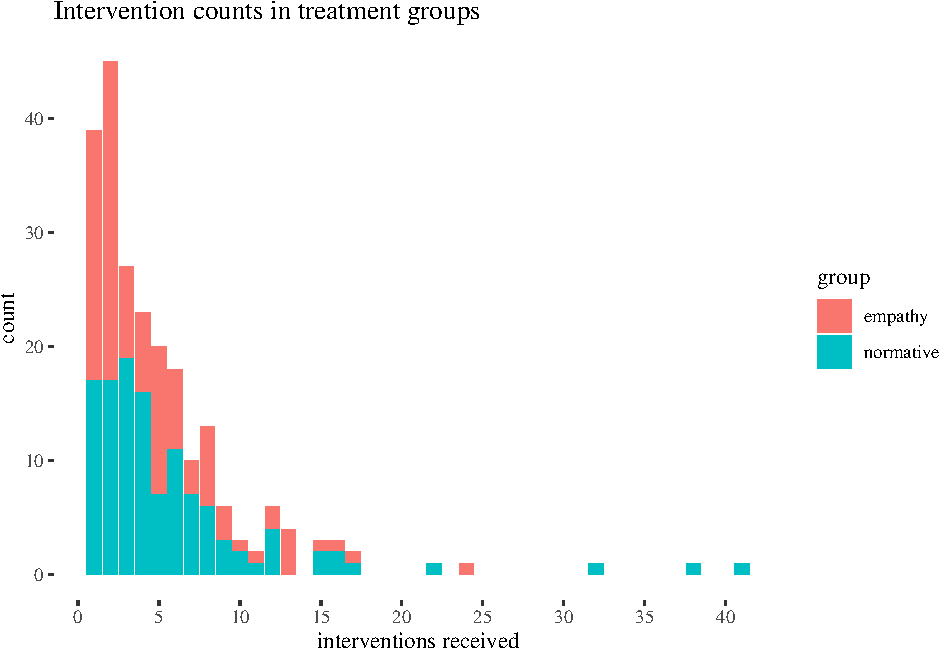
\includegraphics[width=1\linewidth]{bayesianReport3_files/figure-latex/treatmentHist-1} \end{center}

\normalsize

\todo{Note there were much more empathetic interventions, this needs an explanation}

\todo{Question: intervention counts by group}

Second, when we look at the distribution of standardized difference in
attacks, when restricted to (-1,1), the peaks of distributions are
shifted a bit, with lowest median for the normative group, but not too
much:

\vspace{1mm} \footnotesize

\begin{Shaded}
\begin{Highlighting}[]
\NormalTok{violAdiffS <-}\StringTok{ }\KeywordTok{ggplot}\NormalTok{(summaries, }\KeywordTok{aes}\NormalTok{(}\DataTypeTok{x=}\NormalTok{group, }\DataTypeTok{y =}\NormalTok{ AdiffS))}\OperatorTok{+}
\StringTok{  }\KeywordTok{geom_violin}\NormalTok{() }\OperatorTok{+}\KeywordTok{theme_tufte}\NormalTok{() }
\NormalTok{violJoint <-}\StringTok{ }\KeywordTok{ggarrange}\NormalTok{(violAdiffS}\OperatorTok{+}\KeywordTok{ggtitle}\NormalTok{(}\StringTok{"whole range"}\NormalTok{),}
\NormalTok{              violAdiffS }\OperatorTok{+}\StringTok{ }\KeywordTok{ylim}\NormalTok{(}\KeywordTok{c}\NormalTok{(}\OperatorTok{-}\DecValTok{1}\NormalTok{,}\DecValTok{1}\NormalTok{))}\OperatorTok{+}\KeywordTok{geom_boxplot}\NormalTok{(}\DataTypeTok{width =} \FloatTok{.2}\NormalTok{)}\OperatorTok{+}
\StringTok{              }\KeywordTok{ggtitle}\NormalTok{(}\StringTok{"restricted to (-1,1)"}\NormalTok{)) }
\end{Highlighting}
\end{Shaded}

\begin{verbatim}
## Warning: Removed 58 rows containing non-finite values (stat_ydensity).
\end{verbatim}

\begin{verbatim}
## Warning: Removed 58 rows containing non-finite values (stat_boxplot).
\end{verbatim}

\begin{Shaded}
\begin{Highlighting}[]
\NormalTok{violJointTitled <-}\StringTok{ }\KeywordTok{annotate_figure}\NormalTok{(violJoint, }
  \DataTypeTok{top =} \KeywordTok{text_grob}\NormalTok{(}\StringTok{"Empirical distribution of change in attacks (standardized)"}\NormalTok{,}
                  \DataTypeTok{size =} \DecValTok{12}\NormalTok{))}
\NormalTok{violJointTitled}
\end{Highlighting}
\end{Shaded}

\begin{center}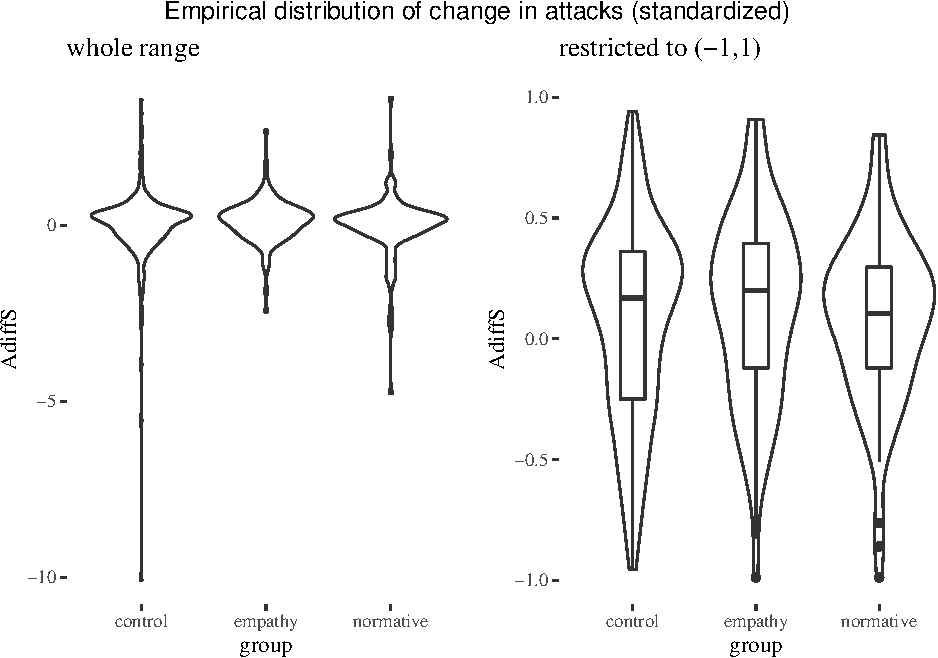
\includegraphics[width=1\linewidth]{bayesianReport3_files/figure-latex/violEmpiricalAdiff-1} \end{center}

\normalsize

Analogous plot for comments does not reveal this slight downward shift
for normative, but otherwise the visualisation migth suggest no strong
impact of interventions on attacks, and no impact on comments.

\vspace{1mm} \footnotesize

\begin{Shaded}
\begin{Highlighting}[]
\NormalTok{violCdiffS <-}\StringTok{ }\KeywordTok{ggplot}\NormalTok{(summaries, }\KeywordTok{aes}\NormalTok{(}\DataTypeTok{x=}\NormalTok{group, }\DataTypeTok{y =}\NormalTok{ CdiffS))}\OperatorTok{+}
\StringTok{  }\KeywordTok{geom_violin}\NormalTok{() }\OperatorTok{+}\KeywordTok{theme_tufte}\NormalTok{() }
\NormalTok{violJointC <-}\StringTok{ }\KeywordTok{ggarrange}\NormalTok{(violCdiffS}\OperatorTok{+}\KeywordTok{ggtitle}\NormalTok{(}\StringTok{"whole range"}\NormalTok{),}
\NormalTok{              violCdiffS }\OperatorTok{+}\StringTok{ }\KeywordTok{ylim}\NormalTok{(}\KeywordTok{c}\NormalTok{(}\OperatorTok{-}\DecValTok{1}\NormalTok{,}\DecValTok{1}\NormalTok{))}\OperatorTok{+}\KeywordTok{geom_boxplot}\NormalTok{(}\DataTypeTok{width =} \FloatTok{.2}\NormalTok{)}\OperatorTok{+}
\StringTok{              }\KeywordTok{ggtitle}\NormalTok{(}\StringTok{"restricted to (-1,1)"}\NormalTok{)) }
\end{Highlighting}
\end{Shaded}

\begin{verbatim}
## Warning: Removed 90 rows containing non-finite values (stat_ydensity).
\end{verbatim}

\begin{verbatim}
## Warning: Removed 90 rows containing non-finite values (stat_boxplot).
\end{verbatim}

\begin{Shaded}
\begin{Highlighting}[]
\NormalTok{violJointCTitled <-}\StringTok{ }\KeywordTok{annotate_figure}\NormalTok{(violJoint, }
  \DataTypeTok{top =} \KeywordTok{text_grob}\NormalTok{(}\StringTok{"Empirical distribution of change in comments (standardized)"}\NormalTok{,}
                  \DataTypeTok{size =} \DecValTok{12}\NormalTok{))}
\NormalTok{violJointCTitled}
\end{Highlighting}
\end{Shaded}

\begin{center}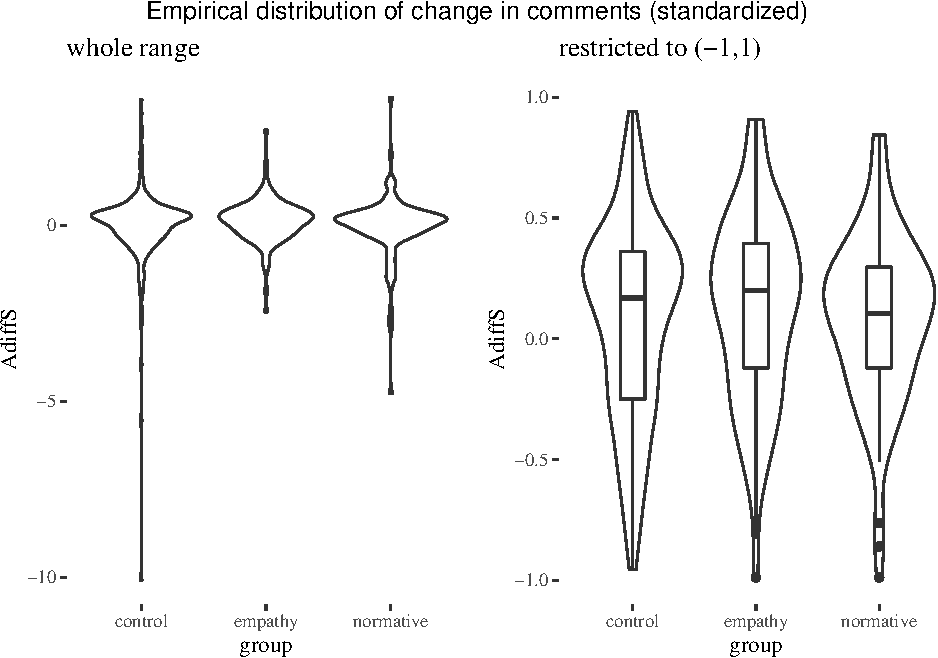
\includegraphics[width=1\linewidth]{bayesianReport3_files/figure-latex/violEpmiricalCdiff-1} \end{center}

\normalsize

However, plotting changes against intervention counts reveals that
restricting attention to various activity levels drastically changes the
regression lines.

\vspace{1mm} \footnotesize

\begin{Shaded}
\begin{Highlighting}[]
\NormalTok{icplot1 <-}\StringTok{ }\KeywordTok{ggplot}\NormalTok{(summaries, }\KeywordTok{aes}\NormalTok{(}\DataTypeTok{x =}\NormalTok{ IC, }\DataTypeTok{y =}\NormalTok{ AdiffS, }\DataTypeTok{color =}\NormalTok{ group, }\DataTypeTok{fill =}\NormalTok{ group))}\OperatorTok{+}
\StringTok{  }\KeywordTok{geom_jitter}\NormalTok{(}\DataTypeTok{alpha =} \FloatTok{0.6}\NormalTok{, }\DataTypeTok{size =}\NormalTok{.}\DecValTok{8}\NormalTok{)}\OperatorTok{+}\KeywordTok{theme_tufte}\NormalTok{()}\OperatorTok{+}
\StringTok{  }\KeywordTok{geom_smooth}\NormalTok{(}\DataTypeTok{alpha =} \FloatTok{0.2}\NormalTok{, }\DataTypeTok{method =} \StringTok{"lm"}\NormalTok{)}\OperatorTok{+}
\StringTok{  }\KeywordTok{xlim}\NormalTok{(}\KeywordTok{c}\NormalTok{(}\DecValTok{0}\NormalTok{,}\DecValTok{25}\NormalTok{))}\OperatorTok{+}\KeywordTok{ylim}\NormalTok{(}\KeywordTok{c}\NormalTok{(}\OperatorTok{-}\DecValTok{2}\NormalTok{,}\DecValTok{2}\NormalTok{))}\OperatorTok{+}
\StringTok{  }\KeywordTok{ggtitle}\NormalTok{(}\StringTok{"sd restricted to (-2,2)"}\NormalTok{)}\OperatorTok{+}
\StringTok{  }\KeywordTok{theme}\NormalTok{(}\DataTypeTok{legend.position =} \KeywordTok{c}\NormalTok{(}\FloatTok{0.65}\NormalTok{, }\FloatTok{0.1}\NormalTok{))}

\NormalTok{icplot2 <-}\StringTok{  }\KeywordTok{ggplot}\NormalTok{(summaries, }\KeywordTok{aes}\NormalTok{(}\DataTypeTok{x =}\NormalTok{ IC, }\DataTypeTok{y =}\NormalTok{ AdiffS, }\DataTypeTok{color =}\NormalTok{ group, }\DataTypeTok{fill =}\NormalTok{ group))}\OperatorTok{+}
\StringTok{  }\KeywordTok{geom_jitter}\NormalTok{(}\DataTypeTok{alpha =} \FloatTok{0.6}\NormalTok{, }\DataTypeTok{size =}\NormalTok{.}\DecValTok{8}\NormalTok{)}\OperatorTok{+}\KeywordTok{theme_tufte}\NormalTok{()}\OperatorTok{+}
\StringTok{  }\KeywordTok{geom_smooth}\NormalTok{(}\DataTypeTok{alpha =} \FloatTok{0.2}\NormalTok{, }\DataTypeTok{method =} \StringTok{"lm"}\NormalTok{)}\OperatorTok{+}
\StringTok{  }\KeywordTok{xlim}\NormalTok{(}\KeywordTok{c}\NormalTok{(}\DecValTok{0}\NormalTok{,}\DecValTok{25}\NormalTok{))}\OperatorTok{+}\KeywordTok{ylim}\NormalTok{(}\KeywordTok{c}\NormalTok{(}\OperatorTok{-}\DecValTok{1}\NormalTok{,}\DecValTok{1}\NormalTok{))}\OperatorTok{+}\KeywordTok{ggtitle}\NormalTok{(}\StringTok{"sd restricted to (-1,1)"}\NormalTok{)}\OperatorTok{+}
\StringTok{  }\KeywordTok{theme}\NormalTok{(}\DataTypeTok{legend.position =} \KeywordTok{c}\NormalTok{(}\FloatTok{0.65}\NormalTok{, }\FloatTok{0.1}\NormalTok{))}

\NormalTok{icplotJoint <-}\StringTok{ }\KeywordTok{ggarrange}\NormalTok{(icplot1, icplot2) }
\NormalTok{icplotTitled <-}\StringTok{ }\KeywordTok{annotate_figure}\NormalTok{(icplotJoint, }
  \DataTypeTok{top =} \KeywordTok{text_grob}\NormalTok{(}\StringTok{"Change in attacks (standardized) vs interventions received"}\NormalTok{,  }\DataTypeTok{size =} \DecValTok{12}\NormalTok{))}
\NormalTok{icplotTitled}
\end{Highlighting}
\end{Shaded}

\begin{center}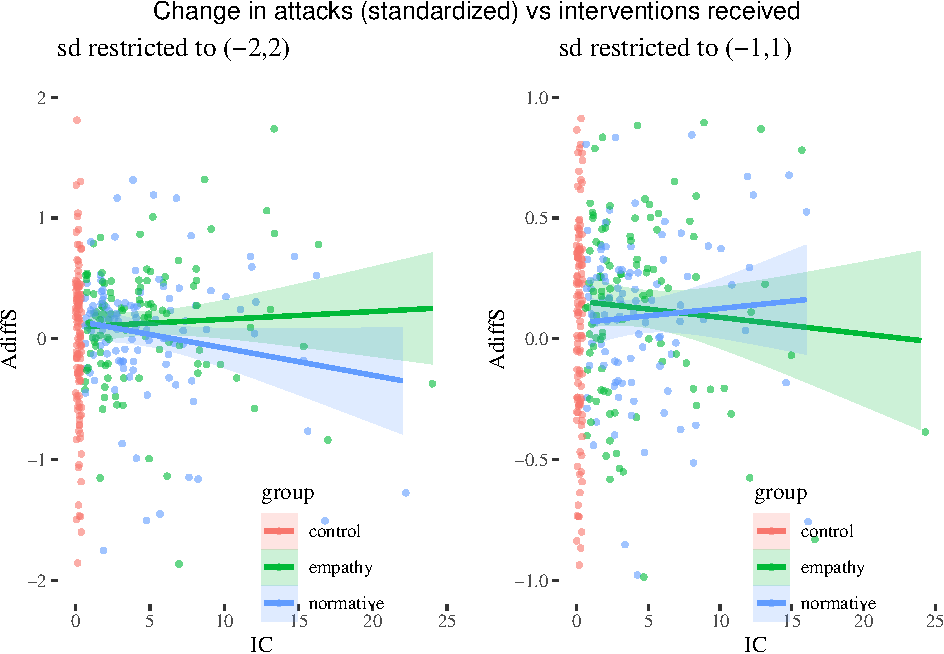
\includegraphics[width=1\linewidth]{bayesianReport3_files/figure-latex/ic-1} \end{center}

\normalsize

Some interactions are also suggested by the differences in linear
smoothing when attention is restricted when it comes to change in
comments.

\vspace{1mm} \footnotesize

\begin{Shaded}
\begin{Highlighting}[]
\NormalTok{icCplot1 <-}\StringTok{ }\KeywordTok{ggplot}\NormalTok{(summaries, }\KeywordTok{aes}\NormalTok{(}\DataTypeTok{x =}\NormalTok{ IC, }\DataTypeTok{y =}\NormalTok{ CdiffS, }\DataTypeTok{color =}\NormalTok{ group, }\DataTypeTok{fill =}\NormalTok{ group))}\OperatorTok{+}
\StringTok{  }\KeywordTok{geom_jitter}\NormalTok{(}\DataTypeTok{alpha =} \FloatTok{0.6}\NormalTok{, }\DataTypeTok{size =}\NormalTok{.}\DecValTok{8}\NormalTok{)}\OperatorTok{+}\KeywordTok{theme_tufte}\NormalTok{()}\OperatorTok{+}
\StringTok{  }\KeywordTok{geom_smooth}\NormalTok{(}\DataTypeTok{alpha =} \FloatTok{0.2}\NormalTok{, }\DataTypeTok{method =} \StringTok{"lm"}\NormalTok{)}\OperatorTok{+}
\StringTok{  }\KeywordTok{xlim}\NormalTok{(}\KeywordTok{c}\NormalTok{(}\DecValTok{0}\NormalTok{,}\DecValTok{25}\NormalTok{))}\OperatorTok{+}\KeywordTok{ylim}\NormalTok{(}\KeywordTok{c}\NormalTok{(}\OperatorTok{-}\DecValTok{2}\NormalTok{,}\DecValTok{2}\NormalTok{))}\OperatorTok{+}
\StringTok{  }\KeywordTok{ggtitle}\NormalTok{(}\StringTok{"sd restricted to (-2,2)"}\NormalTok{)}\OperatorTok{+}
\StringTok{  }\KeywordTok{theme}\NormalTok{(}\DataTypeTok{legend.position =} \KeywordTok{c}\NormalTok{(}\FloatTok{0.65}\NormalTok{, }\FloatTok{0.1}\NormalTok{))}

\NormalTok{icCplot2 <-}\StringTok{  }\KeywordTok{ggplot}\NormalTok{(summaries, }\KeywordTok{aes}\NormalTok{(}\DataTypeTok{x =}\NormalTok{ IC, }\DataTypeTok{y =}\NormalTok{ CdiffS, }\DataTypeTok{color =}\NormalTok{ group, }\DataTypeTok{fill =}\NormalTok{ group))}\OperatorTok{+}
\StringTok{  }\KeywordTok{geom_jitter}\NormalTok{(}\DataTypeTok{alpha =} \FloatTok{0.6}\NormalTok{, }\DataTypeTok{size =}\NormalTok{.}\DecValTok{8}\NormalTok{)}\OperatorTok{+}\KeywordTok{theme_tufte}\NormalTok{()}\OperatorTok{+}
\StringTok{  }\KeywordTok{geom_smooth}\NormalTok{(}\DataTypeTok{alpha =} \FloatTok{0.2}\NormalTok{, }\DataTypeTok{method =} \StringTok{"lm"}\NormalTok{)}\OperatorTok{+}
\StringTok{  }\KeywordTok{xlim}\NormalTok{(}\KeywordTok{c}\NormalTok{(}\DecValTok{0}\NormalTok{,}\DecValTok{25}\NormalTok{))}\OperatorTok{+}\KeywordTok{ylim}\NormalTok{(}\KeywordTok{c}\NormalTok{(}\OperatorTok{-}\DecValTok{1}\NormalTok{,}\DecValTok{1}\NormalTok{))}\OperatorTok{+}\KeywordTok{ggtitle}\NormalTok{(}\StringTok{"sd restricted to (-1,1)"}\NormalTok{)}\OperatorTok{+}
\StringTok{  }\KeywordTok{theme}\NormalTok{(}\DataTypeTok{legend.position =} \KeywordTok{c}\NormalTok{(}\FloatTok{0.65}\NormalTok{, }\FloatTok{0.1}\NormalTok{))}

\NormalTok{icCplotJoint <-}\StringTok{ }\KeywordTok{ggarrange}\NormalTok{(icCplot1, icCplot2) }
\NormalTok{icCplotTitled <-}\StringTok{ }\KeywordTok{annotate_figure}\NormalTok{(icCplotJoint, }
  \DataTypeTok{top =} \KeywordTok{text_grob}\NormalTok{(}\StringTok{"Change in comments (standardized) vs interventions received"}\NormalTok{,}
   \DataTypeTok{size =} \DecValTok{12}\NormalTok{))}
\NormalTok{icCplotTitled}
\end{Highlighting}
\end{Shaded}

\begin{center}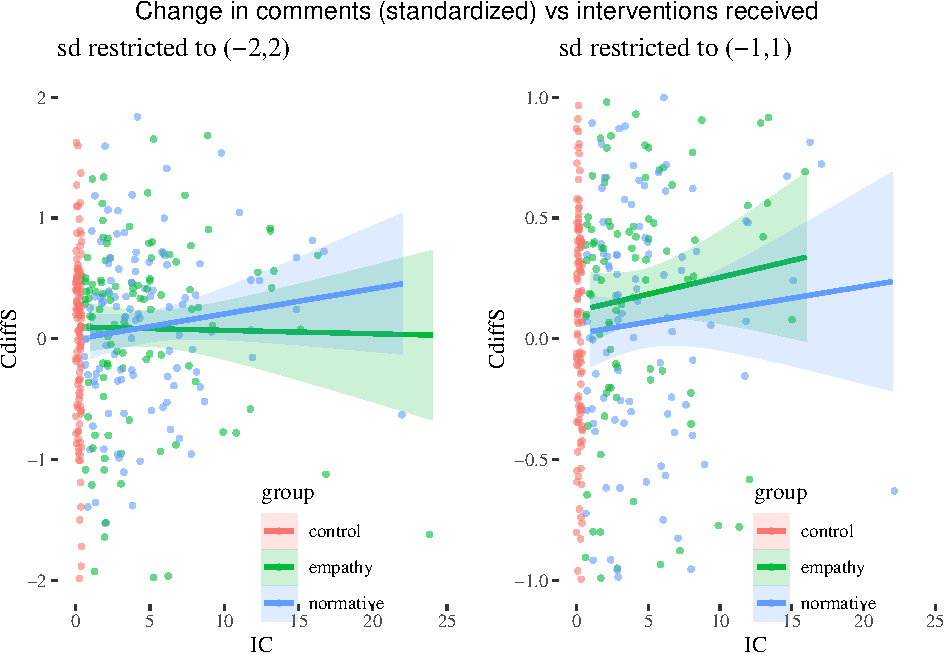
\includegraphics[width=1\linewidth]{bayesianReport3_files/figure-latex/icc-1} \end{center}

\normalsize

This suggests we should keep an eye out for interactions in the
analysis, and that the intial comparison of means or medians between
groups might be misleading if the effects in different volume groups are
different and cancel each other.

Now, let's inspect correlations between the variables involved in the
model:

\vspace{1mm} \footnotesize

\begin{Shaded}
\begin{Highlighting}[]
\NormalTok{summariesCorr <-}\StringTok{ }\KeywordTok{select}\NormalTok{(summaries, IC, ABS, CBS, AAS, CAS, CDS, ADS)}
\KeywordTok{ggcorr}\NormalTok{(summariesCorr, }\DataTypeTok{method =} \KeywordTok{c}\NormalTok{(}\StringTok{"pairwise"}\NormalTok{),}
       \DataTypeTok{digits =} \DecValTok{4}\NormalTok{, }\DataTypeTok{low =} \StringTok{"steelblue"}\NormalTok{, }\DataTypeTok{mid =} \StringTok{"white"}\NormalTok{,}
       \DataTypeTok{high =} \StringTok{"darkred"}\NormalTok{, }\DataTypeTok{midpoint =}\DecValTok{0}\NormalTok{,}
       \DataTypeTok{geom =} \StringTok{"tile"}\NormalTok{, }\DataTypeTok{label =} \OtherTok{TRUE}\NormalTok{, }\DataTypeTok{label_size=}\DecValTok{4}\NormalTok{, }\DataTypeTok{label_round =}\DecValTok{2}\NormalTok{, }\DataTypeTok{layout.exp =}\DecValTok{1}\NormalTok{,}
       \DataTypeTok{label_alpha =} \OtherTok{FALSE}\NormalTok{,}\DataTypeTok{hjust =} \FloatTok{0.75}\NormalTok{)}
\end{Highlighting}
\end{Shaded}

\begin{center}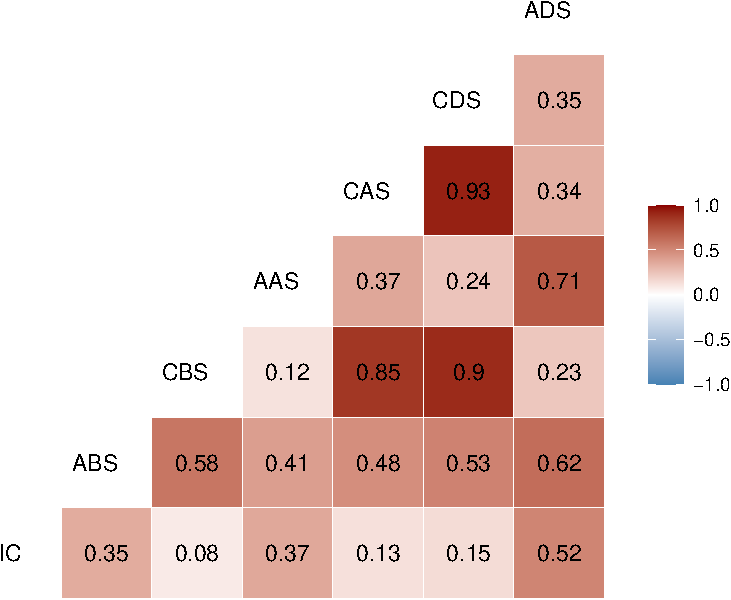
\includegraphics[width=1\linewidth]{bayesianReport3_files/figure-latex/correlations-1} \end{center}

\normalsize

This tells us that almost no predictors are strongly correlated, except
for pairs \textsf{CBS}-\textsf{CDS}, so we drop CDS from the analysis
and avoid using them in the same model to avoid multicolinearity issues.
These are just comments during the intervention period, which,
unsurprisingly are also a good proxy for comments before and comments
after.

\section{Causal inference}\label{causal-inference}

To identify the right variables to condition (or not condition) on to
identify the causal effect of the interventions, we first need to think
about the causal structure of the problem. Here's a plausible causal
structure that we will be working with:

\vspace{1mm} \footnotesize

\begin{Shaded}
\begin{Highlighting}[]
\NormalTok{dag <-}\StringTok{ }\KeywordTok{dagitty}\NormalTok{(}\StringTok{"}
\StringTok{  dag\{}
\StringTok{  CDS -> ADS -> IC  }
\StringTok{               U [unobserved]   }
\StringTok{               U -> CBS -> ABS  }
\StringTok{               U -> ABS        }
\StringTok{               U -> CDS -> ADS  }
\StringTok{               U -> ADS         }
\StringTok{               U -> CAS -> AAS    }
\StringTok{               U -> AAS                        }
\StringTok{               IC -> AAS        }
\StringTok{               IC -> CAS        }
\StringTok{               IT -> CAS        }
\StringTok{               IT -> AAS}
\StringTok{               CBS -> CDS -> CAS}
\StringTok{               ABS -> ADS -> AAS}
\StringTok{               \}"}\NormalTok{)}
\KeywordTok{coordinates}\NormalTok{(dag)}
\end{Highlighting}
\end{Shaded}

\begin{verbatim}
## $x
## AAS ABS ADS CAS CBS CDS  IC  IT   U 
##  NA  NA  NA  NA  NA  NA  NA  NA  NA 
## 
## $y
## AAS ABS ADS CAS CBS CDS  IC  IT   U 
##  NA  NA  NA  NA  NA  NA  NA  NA  NA
\end{verbatim}

\begin{Shaded}
\begin{Highlighting}[]
\KeywordTok{coordinates}\NormalTok{( dag ) <-}\StringTok{ }\KeywordTok{list}\NormalTok{( }\DataTypeTok{x=}\KeywordTok{c}\NormalTok{(}\DataTypeTok{CBS=}\DecValTok{0}\NormalTok{,}\DataTypeTok{ABS=}\DecValTok{0}\NormalTok{,}\DataTypeTok{CDS=}\DecValTok{1}\NormalTok{,}\DataTypeTok{ADS=}\DecValTok{1}\NormalTok{, }\DataTypeTok{CAS =} \DecValTok{2}\NormalTok{,}
                    \DataTypeTok{AAS =} \DecValTok{2}\NormalTok{, }\DataTypeTok{IT =} \FloatTok{1.5}\NormalTok{, }\DataTypeTok{IC =} \FloatTok{1.5}\NormalTok{, }\DataTypeTok{U =} \FloatTok{.5}\NormalTok{) ,}
\DataTypeTok{y=}\KeywordTok{c}\NormalTok{(}\DataTypeTok{CBS =}\DecValTok{0}\NormalTok{,}\DataTypeTok{ABS =} \DecValTok{1}\NormalTok{,}\DataTypeTok{CDS =} \DecValTok{0}\NormalTok{,}\DataTypeTok{ADS =} \DecValTok{1}\NormalTok{, }\DataTypeTok{CAS =} \DecValTok{0}\NormalTok{, }\DataTypeTok{AAS =} \DecValTok{1}\NormalTok{, }
    \DataTypeTok{IT =} \FloatTok{.3}\NormalTok{, }\DataTypeTok{IC =} \FloatTok{.7}\NormalTok{, }\DataTypeTok{U =}\NormalTok{.}\DecValTok{5}\NormalTok{) )}
\KeywordTok{drawdag}\NormalTok{(dag)}
\end{Highlighting}
\end{Shaded}

\begin{center}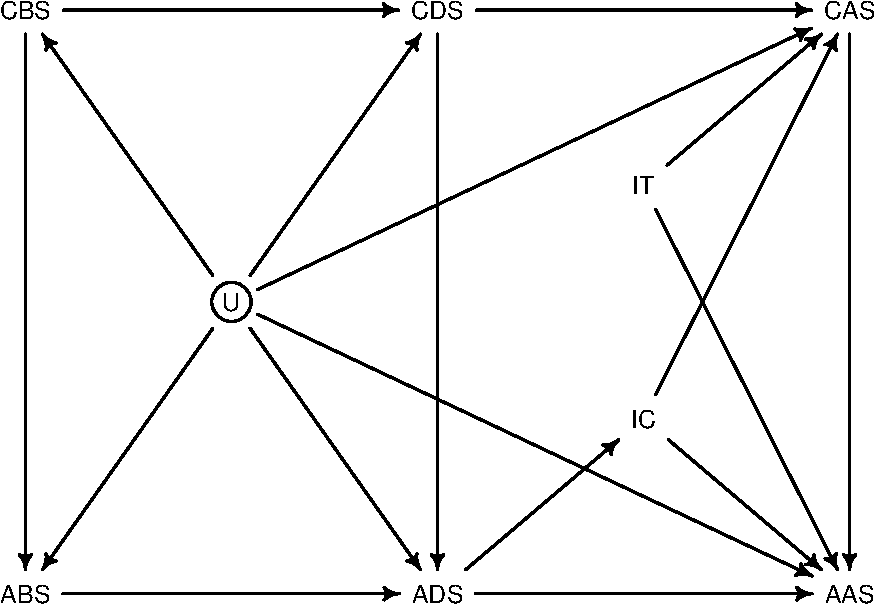
\includegraphics[width=0.8\linewidth]{bayesianReport3_files/figure-latex/dag1-1} \end{center}

\normalsize

Comments during impact attacks during, which trigger interventions.
Unmeasured user features cause comments before, which impact attacks
before, and also attacks before directly. Comments during (their impact
on ADS is areadly included) impact attacks during during directly and
comments after, which impact attacks after and attacks after directly.
Intervention count impacts attacks after and comments after. The same
directions of impact are included for intervention type. Finally,
comments through time are connected causally, and so are attacks.

We already know not to condition on CDS if we condition on CAS or CBS.
What else? \textsf{IT} has no bacwkard paths, but \textsf{IC} does.
Let's identify all paths from \textsf{IC} to \textsf{AAS}:

\vspace{1mm} \footnotesize

\begin{Shaded}
\begin{Highlighting}[]
\KeywordTok{paths}\NormalTok{(dag, }\DataTypeTok{from =} \KeywordTok{c}\NormalTok{(}\StringTok{"IC"}\NormalTok{), }\DataTypeTok{to =} \StringTok{"AAS"}\NormalTok{)}
\end{Highlighting}
\end{Shaded}

\begin{verbatim}
## $paths
##  [1] "IC -> AAS"                                              
##  [2] "IC -> CAS -> AAS"                                       
##  [3] "IC -> CAS <- CDS -> ADS -> AAS"                         
##  [4] "IC -> CAS <- CDS -> ADS <- ABS <- CBS <- U -> AAS"      
##  [5] "IC -> CAS <- CDS -> ADS <- ABS <- U -> AAS"             
##  [6] "IC -> CAS <- CDS -> ADS <- U -> AAS"                    
##  [7] "IC -> CAS <- CDS <- CBS -> ABS -> ADS -> AAS"           
##  [8] "IC -> CAS <- CDS <- CBS -> ABS -> ADS <- U -> AAS"      
##  [9] "IC -> CAS <- CDS <- CBS -> ABS <- U -> AAS"             
## [10] "IC -> CAS <- CDS <- CBS -> ABS <- U -> ADS -> AAS"      
## [11] "IC -> CAS <- CDS <- CBS <- U -> AAS"                    
## [12] "IC -> CAS <- CDS <- CBS <- U -> ABS -> ADS -> AAS"      
## [13] "IC -> CAS <- CDS <- CBS <- U -> ADS -> AAS"             
## [14] "IC -> CAS <- CDS <- U -> AAS"                           
## [15] "IC -> CAS <- CDS <- U -> ABS -> ADS -> AAS"             
## [16] "IC -> CAS <- CDS <- U -> ADS -> AAS"                    
## [17] "IC -> CAS <- CDS <- U -> CBS -> ABS -> ADS -> AAS"      
## [18] "IC -> CAS <- IT -> AAS"                                 
## [19] "IC -> CAS <- U -> AAS"                                  
## [20] "IC -> CAS <- U -> ABS -> ADS -> AAS"                    
## [21] "IC -> CAS <- U -> ABS <- CBS -> CDS -> ADS -> AAS"      
## [22] "IC -> CAS <- U -> ADS -> AAS"                           
## [23] "IC -> CAS <- U -> CBS -> ABS -> ADS -> AAS"             
## [24] "IC -> CAS <- U -> CBS -> CDS -> ADS -> AAS"             
## [25] "IC -> CAS <- U -> CDS -> ADS -> AAS"                    
## [26] "IC -> CAS <- U -> CDS <- CBS -> ABS -> ADS -> AAS"      
## [27] "IC <- ADS -> AAS"                                       
## [28] "IC <- ADS <- ABS <- CBS -> CDS -> CAS -> AAS"           
## [29] "IC <- ADS <- ABS <- CBS -> CDS -> CAS <- IT -> AAS"     
## [30] "IC <- ADS <- ABS <- CBS -> CDS -> CAS <- U -> AAS"      
## [31] "IC <- ADS <- ABS <- CBS -> CDS <- U -> AAS"             
## [32] "IC <- ADS <- ABS <- CBS -> CDS <- U -> CAS -> AAS"      
## [33] "IC <- ADS <- ABS <- CBS -> CDS <- U -> CAS <- IT -> AAS"
## [34] "IC <- ADS <- ABS <- CBS <- U -> AAS"                    
## [35] "IC <- ADS <- ABS <- CBS <- U -> CAS -> AAS"             
## [36] "IC <- ADS <- ABS <- CBS <- U -> CAS <- IT -> AAS"       
## [37] "IC <- ADS <- ABS <- CBS <- U -> CDS -> CAS -> AAS"      
## [38] "IC <- ADS <- ABS <- CBS <- U -> CDS -> CAS <- IT -> AAS"
## [39] "IC <- ADS <- ABS <- U -> AAS"                           
## [40] "IC <- ADS <- ABS <- U -> CAS -> AAS"                    
## [41] "IC <- ADS <- ABS <- U -> CAS <- IT -> AAS"              
## [42] "IC <- ADS <- ABS <- U -> CBS -> CDS -> CAS -> AAS"      
## [43] "IC <- ADS <- ABS <- U -> CBS -> CDS -> CAS <- IT -> AAS"
## [44] "IC <- ADS <- ABS <- U -> CDS -> CAS -> AAS"             
## [45] "IC <- ADS <- ABS <- U -> CDS -> CAS <- IT -> AAS"       
## [46] "IC <- ADS <- CDS -> CAS -> AAS"                         
## [47] "IC <- ADS <- CDS -> CAS <- IT -> AAS"                   
## [48] "IC <- ADS <- CDS -> CAS <- U -> AAS"                    
## [49] "IC <- ADS <- CDS <- CBS -> ABS <- U -> AAS"             
## [50] "IC <- ADS <- CDS <- CBS -> ABS <- U -> CAS -> AAS"      
## [51] "IC <- ADS <- CDS <- CBS -> ABS <- U -> CAS <- IT -> AAS"
## [52] "IC <- ADS <- CDS <- CBS <- U -> AAS"                    
## [53] "IC <- ADS <- CDS <- CBS <- U -> CAS -> AAS"             
## [54] "IC <- ADS <- CDS <- CBS <- U -> CAS <- IT -> AAS"       
## [55] "IC <- ADS <- CDS <- U -> AAS"                           
## [56] "IC <- ADS <- CDS <- U -> CAS -> AAS"                    
## [57] "IC <- ADS <- CDS <- U -> CAS <- IT -> AAS"              
## [58] "IC <- ADS <- U -> AAS"                                  
## [59] "IC <- ADS <- U -> ABS <- CBS -> CDS -> CAS -> AAS"      
## [60] "IC <- ADS <- U -> ABS <- CBS -> CDS -> CAS <- IT -> AAS"
## [61] "IC <- ADS <- U -> CAS -> AAS"                           
## [62] "IC <- ADS <- U -> CAS <- IT -> AAS"                     
## [63] "IC <- ADS <- U -> CBS -> CDS -> CAS -> AAS"             
## [64] "IC <- ADS <- U -> CBS -> CDS -> CAS <- IT -> AAS"       
## [65] "IC <- ADS <- U -> CDS -> CAS -> AAS"                    
## [66] "IC <- ADS <- U -> CDS -> CAS <- IT -> AAS"              
## 
## $open
##  [1]  TRUE  TRUE FALSE FALSE FALSE FALSE FALSE FALSE FALSE FALSE FALSE FALSE
## [13] FALSE FALSE FALSE FALSE FALSE FALSE FALSE FALSE FALSE FALSE FALSE FALSE
## [25] FALSE FALSE  TRUE  TRUE FALSE FALSE FALSE FALSE FALSE  TRUE  TRUE FALSE
## [37]  TRUE FALSE  TRUE  TRUE FALSE  TRUE FALSE  TRUE FALSE  TRUE FALSE FALSE
## [49] FALSE FALSE FALSE  TRUE  TRUE FALSE  TRUE  TRUE FALSE  TRUE FALSE FALSE
## [61]  TRUE FALSE  TRUE FALSE  TRUE FALSE
\end{verbatim}

\normalsize

Crucially, all backdoor paths go through \textsf{ADS}, which then
becomes either a fork or a pipe, so all backdoor paths can be closed by
conditioning on \textsf{ADS}. Moreover there is only one directed
indirect path, it goes through \textsf{CAS}, so we should not condition
on it if we are to identify causal effect on attacks mediated by impact
on comments (unless we care about the direct effect of \textsf{IC} and
\textsf{IT} on \textsf{AAS}, but that's a separate question). This is in
line with the adjustment set identified algorithmically.

\vspace{1mm} \footnotesize

\begin{Shaded}
\begin{Highlighting}[]
\KeywordTok{adjustmentSets}\NormalTok{(dag, }\DataTypeTok{exposure =} \KeywordTok{c}\NormalTok{(}\StringTok{"IC"}\NormalTok{, }\StringTok{"IT"}\NormalTok{), }\DataTypeTok{outcome =} \StringTok{"AAS"}\NormalTok{, }\DataTypeTok{type =} \StringTok{"all"}\NormalTok{)}
\end{Highlighting}
\end{Shaded}

\begin{verbatim}
## { ADS }
## { ABS, ADS }
## { ADS, CBS }
## { ABS, ADS, CBS }
## { ADS, CDS }
## { ABS, ADS, CDS }
## { ADS, CBS, CDS }
## { ABS, ADS, CBS, CDS }
## { ADS, U }
## { ABS, ADS, U }
## { ADS, CBS, U }
## { ABS, ADS, CBS, U }
## { ADS, CDS, U }
## { ABS, ADS, CDS, U }
## { ADS, CBS, CDS, U }
## { ABS, ADS, CBS, CDS, U }
\end{verbatim}

\normalsize

The situation is different when it comes to evaluating the \emph{direct}
effect of intervention. Then, we also need to block indirect causal
paths from the intervention to the outcome. For such an evaluation we
need to also condition on \textsf{CAS}, which is what we will do when we
turn to the study of the direct effects of the interventions.

In fact, we will be predicting the difference between attacks before and
after, and the difference between comments, before and after. Let's add
them to the dag to double-check our selection of variables.

\begin{Shaded}
\begin{Highlighting}[]
\NormalTok{dag2 <-}\StringTok{ }\KeywordTok{dagitty}\NormalTok{(}\StringTok{"}
\StringTok{  dag\{}
\StringTok{                CDS -> ADS -> IC  }
\StringTok{                U [unobserved]   }
\StringTok{                U -> CBS -> ABS  }
\StringTok{                U -> ABS        }
\StringTok{                U -> CDS -> ADS  }
\StringTok{                U -> ADS         }
\StringTok{                U -> CAS -> AAS    }
\StringTok{                U -> AAS                        }
\StringTok{                IC -> AAS        }
\StringTok{                IC -> CAS        }
\StringTok{                IT -> CAS        }
\StringTok{                IT -> AAS}
\StringTok{                CBS -> CDS -> CAS}
\StringTok{                ABS -> ADS -> AAS}
\StringTok{                ABS -> AdiffS}
\StringTok{                AAS -> AdiffS}
\StringTok{                CBS -> CdiffS}
\StringTok{                CAS -> CdiffS}
\StringTok{                \}"}\NormalTok{)}
\KeywordTok{coordinates}\NormalTok{( dag2 ) <-}\StringTok{ }\KeywordTok{list}\NormalTok{( }\DataTypeTok{x=}\KeywordTok{c}\NormalTok{(}\DataTypeTok{CBS=}\DecValTok{0}\NormalTok{,}\DataTypeTok{ABS=}\DecValTok{0}\NormalTok{,}\DataTypeTok{CDS=}\DecValTok{1}\NormalTok{,}\DataTypeTok{ADS=}\DecValTok{1}\NormalTok{,}
    \DataTypeTok{CAS =} \DecValTok{2}\NormalTok{, }\DataTypeTok{AAS =} \DecValTok{2}\NormalTok{, }\DataTypeTok{IT =} \FloatTok{1.5}\NormalTok{, }\DataTypeTok{IC =} \FloatTok{1.5}\NormalTok{, }\DataTypeTok{U =} \FloatTok{.5}\NormalTok{, }\DataTypeTok{AdiffS=} \FloatTok{2.5}\NormalTok{, }\DataTypeTok{CdiffS =} \FloatTok{2.5}\NormalTok{) ,}
\DataTypeTok{y=}\KeywordTok{c}\NormalTok{(}\DataTypeTok{CBS =}\DecValTok{0}\NormalTok{,}\DataTypeTok{ABS =} \DecValTok{1}\NormalTok{,}\DataTypeTok{CDS =} \DecValTok{0}\NormalTok{,}\DataTypeTok{ADS =} \DecValTok{1}\NormalTok{, }\DataTypeTok{CAS =} \DecValTok{0}\NormalTok{, }\DataTypeTok{AAS =} \DecValTok{1}\NormalTok{, }\DataTypeTok{IT =} \FloatTok{.3}\NormalTok{, }\DataTypeTok{IC =} \FloatTok{.7}\NormalTok{, }\DataTypeTok{U =}\NormalTok{.}\DecValTok{5}\NormalTok{, }\DataTypeTok{CdiffS =} \FloatTok{-.2}\NormalTok{,  }\DataTypeTok{AdiffS =} \FloatTok{1.2}\NormalTok{) )}

\KeywordTok{drawdag}\NormalTok{(dag2)}
\KeywordTok{adjustmentSets}\NormalTok{(dag2, }\DataTypeTok{exposure =} \KeywordTok{c}\NormalTok{(}\StringTok{"IC"}\NormalTok{, }\StringTok{"IT"}\NormalTok{), }\DataTypeTok{outcome =} \StringTok{"AdiffS"}\NormalTok{, }\DataTypeTok{type =} \StringTok{"canonical"}\NormalTok{)}
\end{Highlighting}
\end{Shaded}

\begin{verbatim}
## { ABS, ADS, CBS, CDS }
\end{verbatim}

\begin{center}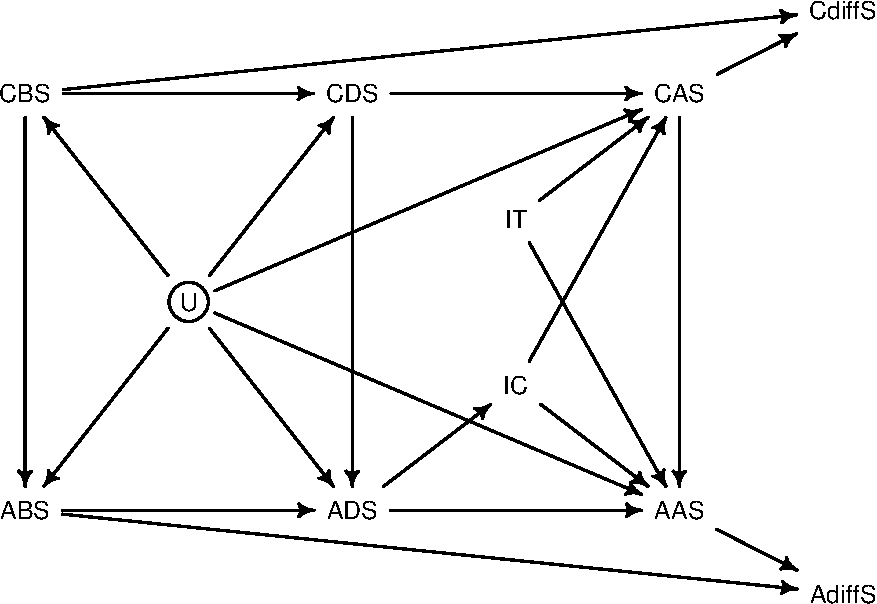
\includegraphics[width=0.8\linewidth]{bayesianReport3_files/figure-latex/dag2-1} \end{center}

Finding a maximal sensible set (canonical) of covariates suggests
inlcuding \textsf{CDS} and \textsf{ABS}. As already discussed, we do not
include \textsf{CDS} because of its strong correlation with
\textsf{CBS}. We also do not condition on \textsf{ABS}---not only
because it has a pretty strong correlation with another predictor
(\textsf{ADS}), but rather mainly because it is used to define the
output variable. In such a set-up, of course that a model including
\textsf{ABS} would have better predictive power, but since a
definitional connection is present, thinking that its inclusion in the
model tells us something about causality would be misled.

It's open season for the other variables (and interactions between
them), and our decision to include them in the model will be guided by
information-theoretic criteria of predictive power.

We will focus on a class of additive models where the outcome variable
is normally distributed around the predicted mean, which is a linear
function of predictors (possibly with some interactions). To spoil the
story, we will end up using a model, whose specification is as follows:

\begin{align*}
\mathsf{AdiffS} & \sim \textsf{Norm}(\mu, \sigma)\\
\mu_i & = \alpha + \beta_{\mathsf{ADS}}[\mathsf{group}_i]\times \mathsf{ADS} + \beta_{\mathsf{group}_i}  +
 \beta_{\mathsf{IC}}[\mathsf{group}_i]\times \mathsf{IC} + \\
 & + \beta_{\mathsf{ADSIC}}\times \mathsf{ADS} \times \mathsf{IC} + \beta_{\mathsf{CBS}}[\mathsf{group}_i] \times \mathsf{CBS}\\
 \alpha & \sim \textsf{Norm}(0,.3)\\
\beta_{\mathsf{ADS}}[\mathsf{group}_i] & \sim \textsf{Norm}(0,.3)\\
\beta_{\mathsf{group}_i} & \sim \textsf{Norm}(0,.3)\\
\beta_{\mathsf{IC}}[\mathsf{group}_i] & \sim \textsf{Norm}(0,.3)\\
 \beta_{\mathsf{ADSIC}} & \sim \textsf{Norm}(0,.3)\\
 \beta_{\mathsf{CBS}}[\mathsf{group}_i]& \sim \textsf{Norm}(0,.3)\\
\end{align*}

That is, we take the resulting mean to be the result of the general
average (\(\alpha\)) and the impact of the following coefficients:
group-specific coefficient for \textsf{ADS}, group coefficient,
group-specific coefficient for \textsf{IC}, interaction coefficient for
\textsf{ADS} and \textsf{IC}, and group-specific coeffient for
\textsf{CBS}. This is plausible prima facie which group a user belongs
to might have impact on how attacks during the treatment is related to
attacks after, the role of the intervention count, and the role of
comments before. Moreover, the levels of agressive behavior displayed by
the user during treament might have impact on the role played by the
intervention count. Later on we will see that there are
information-theoretic reasons to include these interactions.

Now for the priors. One might be suspicious of \(\sigma =.3\) we
employed and suggest using standard normal distributions with
\(\sigma = 1\) instead. However, a quick prior predictive check shows
that this results in insanely wide priors that are competely
unrealistic. (For computational reasons, instead of running the
simulations, we load pre-compiled models, but we include the code used
to build them).

\vspace{1mm} \footnotesize

\begin{Shaded}
\begin{Highlighting}[]
\CommentTok{# building model with sd=1}
\CommentTok{# InteractionsModelDiffSD1 <- ulam(}
\CommentTok{#   alist(}
\CommentTok{#     AdiffS ~ dnorm( mu, sigma ),}
\CommentTok{#     mu <- a + bADS[groupID] * ADS +  bIT[groupID] + bIC[groupID] * IC+}
\CommentTok{#     bADSIC * ADS * IC+ bCBS[groupID] *CBS,}
\CommentTok{#     a ~ dnorm (0,1),}
\CommentTok{#     bADS[groupID] ~ dnorm(0,1),}
\CommentTok{#     bADSIC ~ dnorm(0,1),}
\CommentTok{#     bCBS[groupID] ~ dnorm(0,1),}
\CommentTok{#     bIT[groupID] ~ dnorm(0,1),}
\CommentTok{#     bIC[groupID] ~ dnorm(0,1),}
\CommentTok{#     sigma  ~ dexp(1)}
\CommentTok{#   ), }
\CommentTok{#   data = summaries}
\CommentTok{# )}
\CommentTok{# }
\CommentTok{# saveRDS(InteractionsModelDiffSD1, file = "models/InteractionsModelDiffSD1.rds")}
\NormalTok{InteractionsModelDiffSD1 <-}\StringTok{ }\KeywordTok{readRDS}\NormalTok{(}\DataTypeTok{file =} \StringTok{"models/InteractionsModelDiffSD1.rds"}\NormalTok{)}


\CommentTok{#now model with prior sd = .3}
\CommentTok{# InteractionsModelDiff <- ulam(}
\CommentTok{#   alist(}
\CommentTok{#     AdiffS ~ dnorm( mu, sigma ),}
\CommentTok{#     mu <- a + bADS[groupID] * ADS +  bIT[groupID] + bIC[groupID] * IC +}
\CommentTok{#     bADSIC * ADS * IC+ bCBS[groupID] *CBS,}
\CommentTok{#     a ~ dnorm (0,0.3),}
\CommentTok{#     bADS[groupID] ~ dnorm(0,.3),}
\CommentTok{#     bADSIC ~ dnorm(0,.3),}
\CommentTok{#     bCBS[groupID] ~ dnorm(0,.3),}
\CommentTok{#     bIT[groupID] ~ dnorm(0,.3),}
\CommentTok{#     bIC[groupID] ~ dnorm(0,.3),}
\CommentTok{#     sigma  ~ dexp(1)}
\CommentTok{#   ), }
\CommentTok{#   data = summaries}
\CommentTok{# )}

\CommentTok{#saveRDS(InteractionsModelDiff, file = "models/InteractionsModelDiff.rds")}

\NormalTok{InteractionsModelDiff <-}\StringTok{ }\KeywordTok{readRDS}\NormalTok{(}\DataTypeTok{file =} \StringTok{"models/InteractionsModelDiff.rds"}\NormalTok{)}

\NormalTok{##prior predictive checks sd =1}
\NormalTok{ADS <-}\StringTok{ }\DecValTok{0}
\NormalTok{CBS <-}\StringTok{ }\DecValTok{0}
\NormalTok{groupID <-}\StringTok{ }\DecValTok{1}\OperatorTok{:}\DecValTok{3}
\NormalTok{IC <-}\StringTok{ }\DecValTok{5}  \CommentTok{#mean for interventions in treatment}
\NormalTok{data <-}\StringTok{ }\KeywordTok{expand.grid}\NormalTok{(}\DataTypeTok{ADS =}\NormalTok{ ADS,}\DataTypeTok{groupID =}\NormalTok{ groupID, }\DataTypeTok{CBS =}\NormalTok{ CBS, }\DataTypeTok{IC =}\NormalTok{  IC)}
\NormalTok{prior <-}\StringTok{ }\KeywordTok{extract.prior}\NormalTok{(InteractionsModelDiffSD1, }\DataTypeTok{n =} \FloatTok{1e4}\NormalTok{)}
\NormalTok{mu <-}\StringTok{ }\KeywordTok{link}\NormalTok{( InteractionsModelDiffSD1 , }\DataTypeTok{post=}\NormalTok{prior , }\DataTypeTok{data=}\NormalTok{data ) }
\KeywordTok{colnames}\NormalTok{(mu) <-}\StringTok{ }\KeywordTok{levels}\NormalTok{(summaries}\OperatorTok{$}\NormalTok{group)}
\NormalTok{muLong <-}\StringTok{ }\KeywordTok{melt}\NormalTok{(mu)}
\KeywordTok{colnames}\NormalTok{(muLong) <-}\StringTok{ }\KeywordTok{c}\NormalTok{(}\StringTok{"id"}\NormalTok{, }\StringTok{"group"}\NormalTok{, }\StringTok{"AdiffS"}\NormalTok{)}

\NormalTok{priorGroupsSD1 <-}\StringTok{ }\KeywordTok{ggplot}\NormalTok{(muLong)}\OperatorTok{+}
\StringTok{  }\KeywordTok{geom_violin}\NormalTok{(}\KeywordTok{aes}\NormalTok{(}\DataTypeTok{x =}\NormalTok{ group, }\DataTypeTok{y =}\NormalTok{ AdiffS))}\OperatorTok{+}
\StringTok{  }\KeywordTok{theme_tufte}\NormalTok{()}\OperatorTok{+}\KeywordTok{xlab}\NormalTok{(}\StringTok{""}\NormalTok{)}\OperatorTok{+}
\StringTok{  }\KeywordTok{labs}\NormalTok{(}\DataTypeTok{title =} \StringTok{"Simulated priors by group"}\NormalTok{,}
  \DataTypeTok{subtitle =} \StringTok{"(at ADS = CBS = 0, IC at mean = 5, sd = 1)"}\NormalTok{)}\OperatorTok{+}
\StringTok{  }\KeywordTok{ylab}\NormalTok{(}\StringTok{"change in attacks (standardized)"}\NormalTok{)}

\NormalTok{ADS <-}\StringTok{ }\DecValTok{0}
\NormalTok{CBS <-}\StringTok{ }\DecValTok{0}
\NormalTok{groupID <-}\StringTok{ }\DecValTok{1}\OperatorTok{:}\DecValTok{3}
\NormalTok{IC <-}\StringTok{ }\DecValTok{0}\OperatorTok{:}\DecValTok{20}
\NormalTok{data <-}\StringTok{ }\KeywordTok{expand.grid}\NormalTok{(}\DataTypeTok{ADS =}\NormalTok{ ADS,}\DataTypeTok{groupID =}\NormalTok{ groupID, }\DataTypeTok{CBS =}\NormalTok{ CBS, }\DataTypeTok{IC =}\NormalTok{  IC)}

\NormalTok{prior <-}\StringTok{ }\KeywordTok{extract.prior}\NormalTok{(InteractionsModelDiffSD1, }\DataTypeTok{n =} \FloatTok{1e4}\NormalTok{)}
\end{Highlighting}
\end{Shaded}

\begin{verbatim}
## recompiling to avoid crashing R session
\end{verbatim}

\begin{Shaded}
\begin{Highlighting}[]
\NormalTok{mu <-}\StringTok{ }\KeywordTok{link}\NormalTok{(InteractionsModelDiffSD1 , }\DataTypeTok{post=}\NormalTok{prior , }\DataTypeTok{data=}\NormalTok{data ) }
\NormalTok{mu.mean <-}\StringTok{ }\KeywordTok{apply}\NormalTok{( mu , }\DecValTok{2}\NormalTok{, mean )}
\NormalTok{mu.HPDI <-}\StringTok{ }\KeywordTok{data.frame}\NormalTok{(}\KeywordTok{t}\NormalTok{(}\KeywordTok{apply}\NormalTok{( mu , }\DecValTok{2}\NormalTok{ , HPDI )))}
\NormalTok{priorDF <-}\StringTok{ }\KeywordTok{cbind}\NormalTok{(data, mu.mean, mu.HPDI)}
\NormalTok{priorDF}\OperatorTok{$}\NormalTok{groupID <-}\StringTok{ }\KeywordTok{as.factor}\NormalTok{(groupID)}
\KeywordTok{levels}\NormalTok{(priorDF}\OperatorTok{$}\NormalTok{groupID) <-}\StringTok{ }\KeywordTok{c}\NormalTok{(}\StringTok{"control"}\NormalTok{, }\StringTok{"empathy"}\NormalTok{, }\StringTok{"normative"}\NormalTok{)}
\KeywordTok{colnames}\NormalTok{(priorDF)[}\DecValTok{2}\NormalTok{]<-}\StringTok{ "group"}


\NormalTok{priorICSD1  <-}\StringTok{ }\KeywordTok{ggplot}\NormalTok{(priorDF, }\KeywordTok{aes}\NormalTok{(}\DataTypeTok{x =}\NormalTok{ IC, }\DataTypeTok{y  =}\NormalTok{ mu.mean,  }\DataTypeTok{fill =}\NormalTok{ group))}\OperatorTok{+}
\StringTok{  }\KeywordTok{geom_line}\NormalTok{()}\OperatorTok{+}\KeywordTok{geom_ribbon}\NormalTok{(}\KeywordTok{aes}\NormalTok{(}\DataTypeTok{ymin =}\NormalTok{ X.}\FloatTok{0.89}\NormalTok{, }\DataTypeTok{ymax =}\NormalTok{ X0.}\FloatTok{89.}\NormalTok{), }\DataTypeTok{alpha =} \FloatTok{0.2}\NormalTok{)}\OperatorTok{+}
\StringTok{  }\KeywordTok{theme_tufte}\NormalTok{()}\OperatorTok{+}\KeywordTok{ylab}\NormalTok{(}\StringTok{"change in attacks (standardized)"}\NormalTok{)}\OperatorTok{+}
\StringTok{  }\KeywordTok{labs}\NormalTok{(}\DataTypeTok{title =} \StringTok{"Simulated priors for AAS vs IC"}\NormalTok{,}
      \DataTypeTok{subtitle =} \StringTok{"(at ADS = CBS = 0, sd = 1)"}\NormalTok{)}\OperatorTok{+}\KeywordTok{xlab}\NormalTok{(}\StringTok{"interventions"}\NormalTok{)}


\NormalTok{priorJoint1 <-}\StringTok{ }\KeywordTok{ggarrange}\NormalTok{(priorGroupsSD1,priorICSD1, }\DataTypeTok{ncol =} \DecValTok{2}\NormalTok{) }
\NormalTok{priorJoint1Titled <-}\StringTok{ }\KeywordTok{annotate_figure}\NormalTok{(priorJoint1, }
  \DataTypeTok{top =} \KeywordTok{text_grob}\NormalTok{(}\StringTok{"Predictive priors with sd=1 are insanely wide"}\NormalTok{,}
                  \DataTypeTok{size =} \DecValTok{14}\NormalTok{))}
\NormalTok{priorJoint1Titled}
\end{Highlighting}
\end{Shaded}

\begin{center}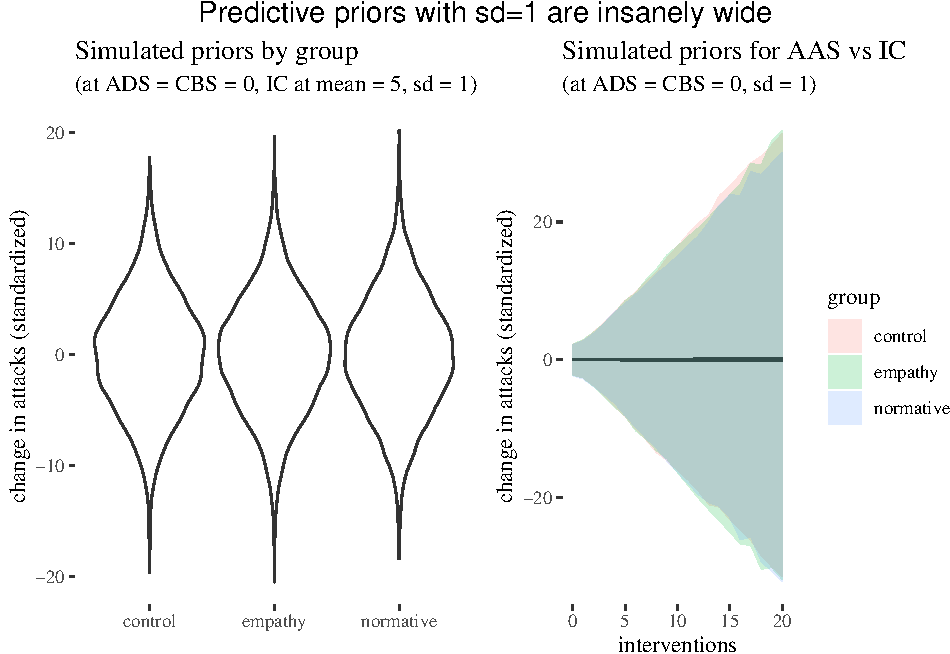
\includegraphics[width=1\linewidth]{bayesianReport3_files/figure-latex/priors1-1} \end{center}

\normalsize

Some experimentation leads to the value of \(\sigma =.3\), which leads
to the following priors:

\vspace{1mm} \footnotesize

\begin{Shaded}
\begin{Highlighting}[]
\CommentTok{#prior predictive check sd =.3}
\NormalTok{ADS <-}\StringTok{ }\DecValTok{0}
\NormalTok{CBS <-}\StringTok{ }\DecValTok{0}
\NormalTok{groupID <-}\StringTok{ }\DecValTok{1}\OperatorTok{:}\DecValTok{3}
\NormalTok{IC <-}\StringTok{ }\DecValTok{5}  \CommentTok{#mean for interventions in treatment}
\NormalTok{data <-}\StringTok{ }\KeywordTok{expand.grid}\NormalTok{(}\DataTypeTok{ADS =}\NormalTok{ ADS,}\DataTypeTok{groupID =}\NormalTok{ groupID, }\DataTypeTok{CBS =}\NormalTok{ CBS, }\DataTypeTok{IC =}\NormalTok{  IC)}
\NormalTok{prior <-}\StringTok{ }\KeywordTok{extract.prior}\NormalTok{(InteractionsModelDiff, }\DataTypeTok{n =} \FloatTok{1e4}\NormalTok{)}
\NormalTok{mu <-}\StringTok{ }\KeywordTok{link}\NormalTok{(InteractionsModelDiff , }\DataTypeTok{post=}\NormalTok{prior , }\DataTypeTok{data=}\NormalTok{data ) }
\KeywordTok{colnames}\NormalTok{(mu) <-}\StringTok{ }\KeywordTok{levels}\NormalTok{(summaries}\OperatorTok{$}\NormalTok{group)}
\NormalTok{muLong <-}\StringTok{ }\KeywordTok{melt}\NormalTok{(mu)}
\KeywordTok{colnames}\NormalTok{(muLong) <-}\StringTok{ }\KeywordTok{c}\NormalTok{(}\StringTok{"id"}\NormalTok{, }\StringTok{"group"}\NormalTok{, }\StringTok{"AdiffS"}\NormalTok{)}
\KeywordTok{head}\NormalTok{(muLong)}

\NormalTok{priorGroupSD03 <-}\StringTok{ }\KeywordTok{ggplot}\NormalTok{(muLong)}\OperatorTok{+}
\StringTok{  }\KeywordTok{geom_violin}\NormalTok{(}\KeywordTok{aes}\NormalTok{(}\DataTypeTok{x =}\NormalTok{ group, }\DataTypeTok{y =}\NormalTok{ AdiffS))}\OperatorTok{+}\KeywordTok{theme_tufte}\NormalTok{()}\OperatorTok{+}
\StringTok{  }\KeywordTok{xlab}\NormalTok{(}\StringTok{""}\NormalTok{)}\OperatorTok{+}
\StringTok{  }\KeywordTok{labs}\NormalTok{(}\DataTypeTok{title =} \StringTok{"Simulated priors  by group"}\NormalTok{, }
  \DataTypeTok{subtitle =} \StringTok{"(at ADS = CBS = 0, IC at mean = 5, sd = .3)"}\NormalTok{)}\OperatorTok{+}
\StringTok{  }\KeywordTok{ylab}\NormalTok{(}\StringTok{"change in attacks (standarized)"}\NormalTok{)}

\NormalTok{ADS <-}\StringTok{ }\DecValTok{0}
\NormalTok{CBS <-}\StringTok{ }\DecValTok{0}
\NormalTok{groupID <-}\StringTok{ }\DecValTok{1}\OperatorTok{:}\DecValTok{3}
\NormalTok{IC <-}\StringTok{ }\DecValTok{5}  \CommentTok{#mean for interventions in treatment}
\NormalTok{data <-}\StringTok{ }\KeywordTok{expand.grid}\NormalTok{(}\DataTypeTok{ADS =}\NormalTok{ ADS,}\DataTypeTok{groupID =}\NormalTok{ groupID, }\DataTypeTok{CBS =}\NormalTok{ CBS, }\DataTypeTok{IC =}\NormalTok{  IC)}
\NormalTok{prior <-}\StringTok{ }\KeywordTok{extract.prior}\NormalTok{(InteractionsModelDiffSD1, }\DataTypeTok{n =} \FloatTok{1e4}\NormalTok{)}
\NormalTok{mu <-}\StringTok{ }\KeywordTok{link}\NormalTok{( InteractionsModelDiffSD1 , }\DataTypeTok{post=}\NormalTok{prior , }\DataTypeTok{data=}\NormalTok{data ) }
\KeywordTok{colnames}\NormalTok{(mu) <-}\StringTok{ }\KeywordTok{levels}\NormalTok{(summaries}\OperatorTok{$}\NormalTok{group)}
\NormalTok{muLong <-}\StringTok{ }\KeywordTok{melt}\NormalTok{(mu)}
\KeywordTok{colnames}\NormalTok{(muLong) <-}\StringTok{ }\KeywordTok{c}\NormalTok{(}\StringTok{"id"}\NormalTok{, }\StringTok{"group"}\NormalTok{, }\StringTok{"AdiffS"}\NormalTok{)}
\KeywordTok{head}\NormalTok{(muLong)}

\NormalTok{priorICSD03 <-}\StringTok{ }\KeywordTok{ggplot}\NormalTok{(muLong)}\OperatorTok{+}
\StringTok{  }\KeywordTok{geom_violin}\NormalTok{(}\KeywordTok{aes}\NormalTok{(}\DataTypeTok{x =}\NormalTok{ group, }\DataTypeTok{y =}\NormalTok{ AdiffS))}\OperatorTok{+}
\StringTok{  }\KeywordTok{theme_tufte}\NormalTok{()}\OperatorTok{+}\KeywordTok{xlab}\NormalTok{(}\StringTok{""}\NormalTok{)}\OperatorTok{+}
\StringTok{  }\KeywordTok{labs}\NormalTok{(}\DataTypeTok{title =} \StringTok{"Simulated priors by group"}\NormalTok{, }
  \DataTypeTok{subtitle =} \StringTok{"(at ADS = CBS = 0, IC at mean = 5, sd = 1)"}\NormalTok{)}\OperatorTok{+}
\StringTok{  }\KeywordTok{ylab}\NormalTok{(}\StringTok{"change in attacks (standardized)"}\NormalTok{)}

\NormalTok{priorJoint03 <-}\StringTok{ }\KeywordTok{ggarrange}\NormalTok{(priorGroupSD03,priorICSD03, }\DataTypeTok{ncol =} \DecValTok{2}\NormalTok{) }
\NormalTok{priorJoint03Titled <-}\StringTok{ }\KeywordTok{annotate_figure}\NormalTok{(priorJoint03, }
  \DataTypeTok{top =} \KeywordTok{text_grob}\NormalTok{(}\StringTok{"Predictive priors with sd=.3 seem sensible"}\NormalTok{,}
                  \DataTypeTok{size =} \DecValTok{14}\NormalTok{))}
\NormalTok{priorJoint03Titled}
\end{Highlighting}
\end{Shaded}

\begin{center}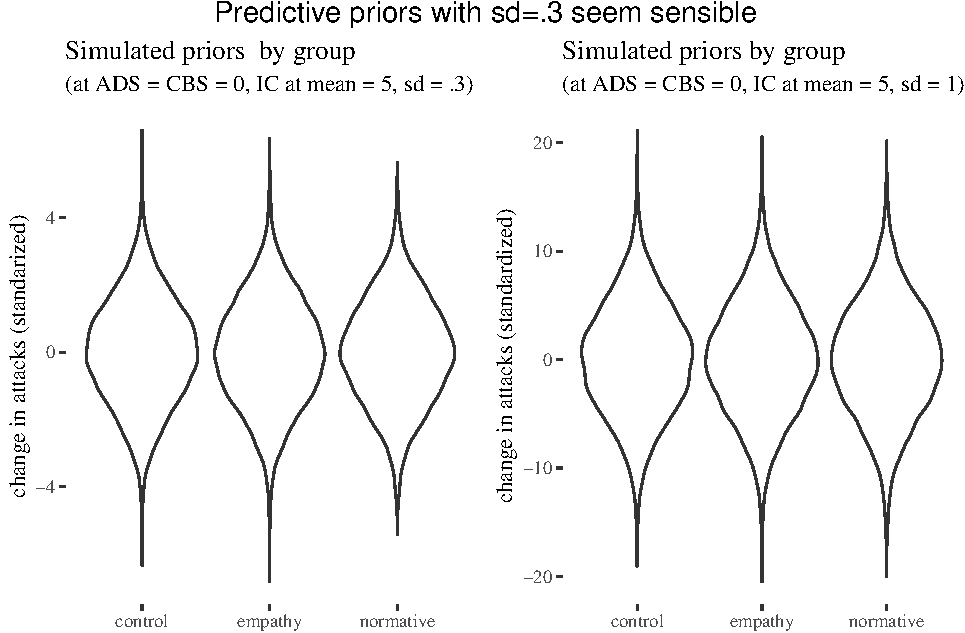
\includegraphics[width=1\linewidth]{bayesianReport3_files/figure-latex/priors03-1} \end{center}

\normalsize

Now, some model diagnostics before we move on. What we are witnessing is
(1) stationarity (the chains stay mostly in the most probable regions),
(2) good mixing (they explore a range of options in the beginning), and
(3) convergence (they stabilize as they progress).

\vspace{1mm} \footnotesize

\begin{Shaded}
\begin{Highlighting}[]
\KeywordTok{traceplot}\NormalTok{( InteractionsModelDiff )}
\end{Highlighting}
\end{Shaded}

\begin{center}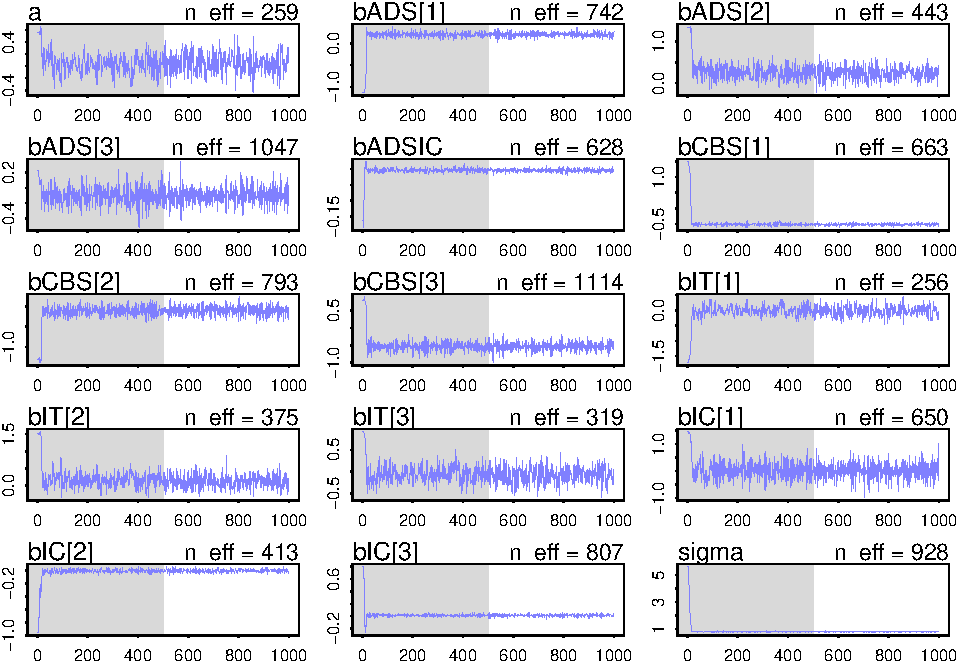
\includegraphics[width=1\linewidth]{bayesianReport3_files/figure-latex/unnamed-chunk-6-1} \end{center}

\normalsize

Finally, let's inspect the distribution of residuals. That is, we
calculate all predictions, their distance from the actual values, and
inspect the distribution of the distances:

\vspace{1mm} \footnotesize

\begin{Shaded}
\begin{Highlighting}[]
\NormalTok{mu <-}\StringTok{ }\KeywordTok{link}\NormalTok{(InteractionsModelDiff)}
\NormalTok{mu_mean <-}\StringTok{ }\KeywordTok{apply}\NormalTok{( mu , }\DecValTok{2}\NormalTok{ , mean )}
\NormalTok{mu_resid <-}\StringTok{ }\NormalTok{summaries}\OperatorTok{$}\NormalTok{AdiffS }\OperatorTok{-}\StringTok{ }\NormalTok{mu_mean}
\KeywordTok{ggplot}\NormalTok{()}\OperatorTok{+}\KeywordTok{geom_density}\NormalTok{(}\KeywordTok{aes}\NormalTok{(}\DataTypeTok{x =}\NormalTok{ mu_resid))}\OperatorTok{+}\KeywordTok{theme_tufte}\NormalTok{()}\OperatorTok{+}
\StringTok{  }\KeywordTok{ggtitle}\NormalTok{(}\StringTok{"Residuals are approximately normally distributed"}\NormalTok{)}\OperatorTok{+}\KeywordTok{xlab}\NormalTok{(}\StringTok{"residuals"}\NormalTok{)}
\end{Highlighting}
\end{Shaded}

\begin{center}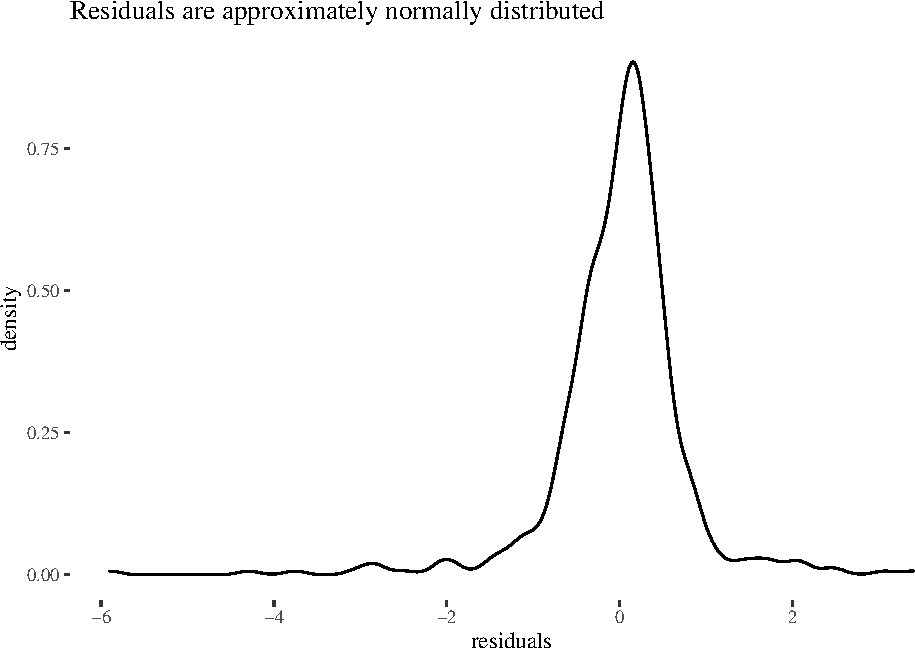
\includegraphics[width=1\linewidth]{bayesianReport3_files/figure-latex/unnamed-chunk-7-1} \end{center}

\normalsize

\section{Model selection}\label{model-selection}

How did we get to this fairly complicated model though? Once preliminary
causal considerations guided our restrictions on variable selection, we
proceed by building models of increasing complexity, and comparing them
in terms of Widely Acceptable Information Criterion. The models differ
mostly in the underlying linear formulae. For computational ease we will
here use quadratic approximations, while in the final analysis we will
deploy Hamiltionian Monte Carlo. The names are meant to decode the model
structure: the predictors are listed before dashes, whereas interactions
are listed after dashes.

\begin{align}
\tag{Null}  \mu_i & = \alpha\\
\tag{ADS}  \mu_i & = \alpha + \beta_{\mathsf{ADS}}\times \mathsf{ADS}\\
\tag{ADSIC}  \mu_i & = \alpha + \beta_{\mathsf{ADS}}\times \mathsf{ADS} +    \beta_{\mathsf{IC}}\times \mathsf{IC}\\
\tag{IT}  \mu_i & = \beta_{\mathsf{group}[i]} \\
\tag{ADSIT} \mu_i & = \alpha + \beta_{\mathsf{ADS}}\times \mathsf{ADS} +  \beta_{\mathsf{group}[i]}\\
\tag{ADSITIC} \mu_i & = \alpha + \beta_{\mathsf{ADS}}\times \mathsf{ADS} +  \beta_{\mathsf{group}[i]} +    \beta_{\mathsf{IC}}\times \mathsf{IC}\\
\tag{ADSITIC-ADSIC} \mu_i & = \alpha + \beta_{\mathsf{ADS}}\times \mathsf{ADS} +  \beta_{\mathsf{group}[i]} +    \beta_{\mathsf{IC}}\times \mathsf{IC} + \beta_{\mathsf{ADSIC}}\times \mathsf{ADS} \times \mathsf{IC}\\
\tag{ADSITIC-ADSIC-ADSIT} \mu_i & = \alpha + \beta_{\mathsf{ADS}}[\mathsf{group}_i]\times \mathsf{ADS} +  \beta_{\mathsf{group}[i]} +  \\ \nonumber & +  \beta_{\mathsf{IC}}\times \mathsf{IC} + \beta_{\mathsf{ADSIC}}\times \mathsf{ADS} \times \mathsf{IC}\\
\tag{ADSIT-ADSIT}   \mu_i &  = \alpha + \beta_{\mathsf{ADS}}[\mathsf{group}_i] \times
 \mathsf{ADS} + \beta_{\mathsf{group}[i]} \\
\tag{ADSITIC-ADSIT-ITIC-ADSIC}   \mu_i &  = \alpha  +  \beta_{\mathsf{ADS}}[\mathsf{group}_i] \times \mathsf{ADS} + \beta_{\mathsf{group}[i]} +  
\beta_{\mathsf{IC}}[\mathsf{group}_i] \times \mathsf{IC} + \\ \nonumber & + \beta_{\mathsf{ADSIC}}\times \mathsf{ADS} \times \mathsf{IC}\\
\tag{ADSITICCBS-ITIC-ADSIC} \mu_i &  = \alpha  +  \beta_{\mathsf{ADS}}[\mathsf{group}_i] \times
 \mathsf{ADS}  + \beta_{\mathsf{group}[i]} +   \beta_{\mathsf{IC}}[\mathsf{group}_i] \times \mathsf{IC} + \\ & \nonumber  + \beta_{\mathsf{CBS}} \times \mathsf{CBS} +  \beta_{\mathsf{ADSIC}}\times \mathsf{ADS} \times \mathsf{IC}  \\
\tag{Final} \mu_i & = \alpha + \beta_{\mathsf{ADS}}[\mathsf{group}_i]\times \mathsf{ADS} + \beta_{\mathsf{group}_i}  +  \beta_{\mathsf{IC}}[\mathsf{group}_i]\times \mathsf{IC} + \\
 & + \beta_{\mathsf{ADSIC}}\times \mathsf{ADS} \times \mathsf{IC} + \beta_{\mathsf{CBS}}[\mathsf{group}_i] \times \mathsf{CBS} \nonumber\\
 \tag{tooFAr} \mu_i & = \alpha + \beta_{\mathsf{ADS}}[\mathsf{group}_i]\times \mathsf{ADS} + \beta_{\mathsf{group}_i}  +  \beta_{\mathsf{IC}}[\mathsf{group}_i]\times \mathsf{IC} + \\
 & + \beta_{\mathsf{ADSIC}}\times \mathsf{ADS} \times \mathsf{IC} + \beta_{\mathsf{CBS}}[\mathsf{group}_i] \times \mathsf{CBS} + \beta_{\mathsf{CBSIC}}\times
 \mathsf{CBS} \times \mathsf{IC}\end{align}

\vspace{1mm} \footnotesize

\begin{Shaded}
\begin{Highlighting}[]
\NormalTok{null <-}\StringTok{ }\KeywordTok{quap}\NormalTok{(}
  \KeywordTok{alist}\NormalTok{(}
\NormalTok{    AdiffS }\OperatorTok{~}\StringTok{ }\KeywordTok{dnorm}\NormalTok{( mu, sigma ),}
\NormalTok{    mu }\OperatorTok{~}\StringTok{ }\KeywordTok{dnorm}\NormalTok{ (}\DecValTok{0}\NormalTok{,}\FloatTok{0.3}\NormalTok{),}
\NormalTok{    sigma  }\OperatorTok{~}\StringTok{ }\KeywordTok{dexp}\NormalTok{(}\DecValTok{1}\NormalTok{)}
\NormalTok{  ), }
  \DataTypeTok{data =}\NormalTok{ summaries  }
\NormalTok{)}

\NormalTok{ADS <-}\StringTok{ }\KeywordTok{quap}\NormalTok{(}
  \KeywordTok{alist}\NormalTok{(}
\NormalTok{    AdiffS }\OperatorTok{~}\StringTok{ }\KeywordTok{dnorm}\NormalTok{( mu, sigma ),}
\NormalTok{    mu <-}\StringTok{  }\NormalTok{a }\OperatorTok{+}\StringTok{ }\NormalTok{bADS }\OperatorTok{*}\StringTok{ }\NormalTok{ADS,}
\NormalTok{    a }\OperatorTok{~}\StringTok{ }\KeywordTok{dnorm}\NormalTok{ (}\DecValTok{0}\NormalTok{,}\FloatTok{0.3}\NormalTok{),}
\NormalTok{    bADS }\OperatorTok{~}\StringTok{ }\KeywordTok{dnorm}\NormalTok{(}\DecValTok{0}\NormalTok{,}\FloatTok{0.3}\NormalTok{),}
\NormalTok{    sigma  }\OperatorTok{~}\StringTok{ }\KeywordTok{dexp}\NormalTok{(}\DecValTok{1}\NormalTok{)}
\NormalTok{  ), }
  \DataTypeTok{data =}\NormalTok{ summaries}
\NormalTok{)}

\NormalTok{ADSIC <-}\StringTok{ }\KeywordTok{quap}\NormalTok{(}
  \KeywordTok{alist}\NormalTok{(}
\NormalTok{    AdiffS }\OperatorTok{~}\StringTok{ }\KeywordTok{dnorm}\NormalTok{( mu, sigma ),}
\NormalTok{    mu <-}\StringTok{  }\NormalTok{a }\OperatorTok{+}\StringTok{ }\NormalTok{bADS }\OperatorTok{*}\StringTok{ }\NormalTok{ADS}\OperatorTok{+}\StringTok{ }\NormalTok{bIC }\OperatorTok{*}\StringTok{ }\NormalTok{IC,}
\NormalTok{    a }\OperatorTok{~}\StringTok{ }\KeywordTok{dnorm}\NormalTok{ (}\DecValTok{0}\NormalTok{,}\FloatTok{0.3}\NormalTok{),}
\NormalTok{    bADS }\OperatorTok{~}\StringTok{ }\KeywordTok{dnorm}\NormalTok{(}\DecValTok{0}\NormalTok{,}\FloatTok{0.3}\NormalTok{),}
\NormalTok{    bIC }\OperatorTok{~}\StringTok{ }\KeywordTok{dnorm}\NormalTok{(}\DecValTok{0}\NormalTok{,}\FloatTok{0.3}\NormalTok{),}
\NormalTok{    sigma  }\OperatorTok{~}\StringTok{ }\KeywordTok{dexp}\NormalTok{(}\DecValTok{1}\NormalTok{)}
\NormalTok{  ), }
  \DataTypeTok{data =}\NormalTok{ summaries}
\NormalTok{)}


\NormalTok{IT <-}\StringTok{ }\KeywordTok{quap}\NormalTok{(}
  \KeywordTok{alist}\NormalTok{(}
\NormalTok{    AdiffS }\OperatorTok{~}\StringTok{ }\KeywordTok{dnorm}\NormalTok{( mu, sigma ),}
\NormalTok{    mu <-}\StringTok{  }\NormalTok{bIT[groupID] ,}
\NormalTok{    bIT[groupID] }\OperatorTok{~}\StringTok{ }\KeywordTok{dnorm}\NormalTok{(}\DecValTok{0}\NormalTok{,.}\DecValTok{3}\NormalTok{),}
\NormalTok{    sigma  }\OperatorTok{~}\StringTok{ }\KeywordTok{dexp}\NormalTok{(}\DecValTok{1}\NormalTok{)}
\NormalTok{  ), }
  \DataTypeTok{data =}\NormalTok{ summaries}
\NormalTok{)}


\NormalTok{ADSIT <-}\StringTok{ }\KeywordTok{quap}\NormalTok{(}
  \KeywordTok{alist}\NormalTok{(}
\NormalTok{    AdiffS }\OperatorTok{~}\StringTok{ }\KeywordTok{dnorm}\NormalTok{( mu, sigma ),}
\NormalTok{    mu <-}\StringTok{ }\NormalTok{a }\OperatorTok{+}\StringTok{ }\NormalTok{bADS }\OperatorTok{*}\StringTok{ }\NormalTok{ADS }\OperatorTok{+}\StringTok{  }\NormalTok{bIT[groupID],}
\NormalTok{    a }\OperatorTok{~}\StringTok{ }\KeywordTok{dnorm}\NormalTok{ (}\DecValTok{0}\NormalTok{,}\FloatTok{0.3}\NormalTok{),}
\NormalTok{    bADS }\OperatorTok{~}\StringTok{ }\KeywordTok{dnorm}\NormalTok{(}\DecValTok{0}\NormalTok{,.}\DecValTok{3}\NormalTok{),}
\NormalTok{    bIT[groupID] }\OperatorTok{~}\StringTok{ }\KeywordTok{dnorm}\NormalTok{(}\DecValTok{0}\NormalTok{,.}\DecValTok{3}\NormalTok{),}
\NormalTok{    sigma  }\OperatorTok{~}\StringTok{ }\KeywordTok{dexp}\NormalTok{(}\DecValTok{1}\NormalTok{)}
\NormalTok{  ), }
  \DataTypeTok{data =}\NormalTok{ summaries}
\NormalTok{)}


\NormalTok{ADSITIC <-}\StringTok{ }\KeywordTok{quap}\NormalTok{(}
  \KeywordTok{alist}\NormalTok{(}
\NormalTok{    AdiffS }\OperatorTok{~}\StringTok{ }\KeywordTok{dnorm}\NormalTok{( mu, sigma ),}
\NormalTok{    mu <-}\StringTok{ }\NormalTok{a }\OperatorTok{+}\StringTok{ }\NormalTok{bADS }\OperatorTok{*}\StringTok{ }\NormalTok{ADS }\OperatorTok{+}\StringTok{  }\NormalTok{bIT[groupID] }\OperatorTok{+}\StringTok{ }\NormalTok{bIC }\OperatorTok{*}\StringTok{ }\NormalTok{IC,}
\NormalTok{    a }\OperatorTok{~}\StringTok{ }\KeywordTok{dnorm}\NormalTok{ (}\DecValTok{0}\NormalTok{,}\FloatTok{0.3}\NormalTok{),}
\NormalTok{    bADS }\OperatorTok{~}\StringTok{ }\KeywordTok{dnorm}\NormalTok{(}\DecValTok{0}\NormalTok{,.}\DecValTok{3}\NormalTok{),}
\NormalTok{    bIT[groupID] }\OperatorTok{~}\StringTok{ }\KeywordTok{dnorm}\NormalTok{(}\DecValTok{0}\NormalTok{,.}\DecValTok{3}\NormalTok{),}
\NormalTok{    bIC }\OperatorTok{~}\StringTok{ }\KeywordTok{dnorm}\NormalTok{(}\DecValTok{0}\NormalTok{,.}\DecValTok{3}\NormalTok{),}
\NormalTok{    sigma  }\OperatorTok{~}\StringTok{ }\KeywordTok{dexp}\NormalTok{(}\DecValTok{1}\NormalTok{)}
\NormalTok{  ), }
  \DataTypeTok{data =}\NormalTok{ summaries}
\NormalTok{)}


\NormalTok{ADSITIC_ADSIC <-}\StringTok{ }\KeywordTok{quap}\NormalTok{(}
  \KeywordTok{alist}\NormalTok{(}
\NormalTok{    AdiffS }\OperatorTok{~}\StringTok{ }\KeywordTok{dnorm}\NormalTok{( mu, sigma ),}
\NormalTok{    mu <-}\StringTok{ }\NormalTok{a }\OperatorTok{+}\StringTok{ }\NormalTok{bADS }\OperatorTok{*}\StringTok{ }\NormalTok{ADS }\OperatorTok{+}\StringTok{  }\NormalTok{bIT[groupID] }\OperatorTok{+}\StringTok{ }\NormalTok{bIC }\OperatorTok{*}\StringTok{ }\NormalTok{IC }\OperatorTok{+}\StringTok{ }\NormalTok{bADSIC }\OperatorTok{*}\StringTok{ }\NormalTok{ADS }\OperatorTok{*}\StringTok{ }\NormalTok{IC,}
\NormalTok{    a }\OperatorTok{~}\StringTok{ }\KeywordTok{dnorm}\NormalTok{ (}\DecValTok{0}\NormalTok{,}\FloatTok{0.3}\NormalTok{),}
\NormalTok{    bADS }\OperatorTok{~}\StringTok{ }\KeywordTok{dnorm}\NormalTok{(}\DecValTok{0}\NormalTok{,.}\DecValTok{3}\NormalTok{),}
\NormalTok{    bADSIC }\OperatorTok{~}\StringTok{ }\KeywordTok{dnorm}\NormalTok{(}\DecValTok{0}\NormalTok{,.}\DecValTok{3}\NormalTok{),}
\NormalTok{    bIT[groupID] }\OperatorTok{~}\StringTok{ }\KeywordTok{dnorm}\NormalTok{(}\DecValTok{0}\NormalTok{,.}\DecValTok{3}\NormalTok{),}
\NormalTok{    bIC }\OperatorTok{~}\StringTok{ }\KeywordTok{dnorm}\NormalTok{(}\DecValTok{0}\NormalTok{,.}\DecValTok{3}\NormalTok{),}
\NormalTok{    sigma  }\OperatorTok{~}\StringTok{ }\KeywordTok{dexp}\NormalTok{(}\DecValTok{1}\NormalTok{)}
\NormalTok{  ), }
  \DataTypeTok{data =}\NormalTok{ summaries}
\NormalTok{)}


\NormalTok{ADSITIC_ADSIC_ADSIT <-}\StringTok{ }\KeywordTok{quap}\NormalTok{(}
  \KeywordTok{alist}\NormalTok{(}
\NormalTok{    AdiffS }\OperatorTok{~}\StringTok{ }\KeywordTok{dnorm}\NormalTok{( mu, sigma ),}
\NormalTok{    mu <-}\StringTok{ }\NormalTok{a }\OperatorTok{+}\StringTok{ }\NormalTok{bADS[groupID] }\OperatorTok{*}\StringTok{ }\NormalTok{ADS }\OperatorTok{+}\StringTok{  }\NormalTok{bIT[groupID] }\OperatorTok{+}\StringTok{ }\NormalTok{bIC }\OperatorTok{*}\StringTok{ }\NormalTok{IC }\OperatorTok{+}\StringTok{ }\NormalTok{bADSIC }\OperatorTok{*}\StringTok{ }\NormalTok{ADS }\OperatorTok{*}\StringTok{ }\NormalTok{IC,}
\NormalTok{    a }\OperatorTok{~}\StringTok{ }\KeywordTok{dnorm}\NormalTok{ (}\DecValTok{0}\NormalTok{,}\FloatTok{0.3}\NormalTok{),}
\NormalTok{    bADS[groupID] }\OperatorTok{~}\StringTok{ }\KeywordTok{dnorm}\NormalTok{(}\DecValTok{0}\NormalTok{,.}\DecValTok{3}\NormalTok{),}
\NormalTok{    bADSIC }\OperatorTok{~}\StringTok{ }\KeywordTok{dnorm}\NormalTok{(}\DecValTok{0}\NormalTok{,.}\DecValTok{3}\NormalTok{),}
\NormalTok{    bIT[groupID] }\OperatorTok{~}\StringTok{ }\KeywordTok{dnorm}\NormalTok{(}\DecValTok{0}\NormalTok{,.}\DecValTok{3}\NormalTok{),}
\NormalTok{    bIC }\OperatorTok{~}\StringTok{ }\KeywordTok{dnorm}\NormalTok{(}\DecValTok{0}\NormalTok{,.}\DecValTok{3}\NormalTok{),}
\NormalTok{    sigma  }\OperatorTok{~}\StringTok{ }\KeywordTok{dexp}\NormalTok{(}\DecValTok{1}\NormalTok{)}
\NormalTok{  ), }
  \DataTypeTok{data =}\NormalTok{ summaries}
\NormalTok{)}


\NormalTok{ADSIT_ADSIT <-}\StringTok{ }\KeywordTok{quap}\NormalTok{(}
  \KeywordTok{alist}\NormalTok{(}
\NormalTok{    AdiffS }\OperatorTok{~}\StringTok{ }\KeywordTok{dnorm}\NormalTok{( mu, sigma ),}
\NormalTok{    mu <-}\StringTok{ }\NormalTok{a }\OperatorTok{+}\StringTok{ }\NormalTok{bADS[groupID] }\OperatorTok{*}\StringTok{ }\NormalTok{ADS }\OperatorTok{+}\StringTok{  }\NormalTok{bIT[groupID] ,}
\NormalTok{    a }\OperatorTok{~}\StringTok{ }\KeywordTok{dnorm}\NormalTok{ (}\DecValTok{0}\NormalTok{,}\FloatTok{0.3}\NormalTok{),}
\NormalTok{    bADS[groupID] }\OperatorTok{~}\StringTok{ }\KeywordTok{dnorm}\NormalTok{(}\DecValTok{0}\NormalTok{,.}\DecValTok{3}\NormalTok{),}
    \CommentTok{#bADSIC ~ dnorm(0,.5),}
\NormalTok{    bIT[groupID] }\OperatorTok{~}\StringTok{ }\KeywordTok{dnorm}\NormalTok{(}\DecValTok{0}\NormalTok{,.}\DecValTok{3}\NormalTok{),}
    \CommentTok{#bIC ~ dnorm(0,.5),}
\NormalTok{    sigma  }\OperatorTok{~}\StringTok{ }\KeywordTok{dexp}\NormalTok{(}\DecValTok{1}\NormalTok{)}
\NormalTok{  ), }
  \DataTypeTok{data =}\NormalTok{ summaries}
\NormalTok{)}


\NormalTok{ADSITIC_ADSIT_ITIC_ADSIC <-}\StringTok{ }\KeywordTok{quap}\NormalTok{(}
  \KeywordTok{alist}\NormalTok{(}
\NormalTok{    AdiffS }\OperatorTok{~}\StringTok{ }\KeywordTok{dnorm}\NormalTok{( mu, sigma ),}
\NormalTok{    mu <-}\StringTok{ }\NormalTok{a }\OperatorTok{+}\StringTok{ }\NormalTok{bADS[groupID] }\OperatorTok{*}\StringTok{ }\NormalTok{ADS }\OperatorTok{+}\StringTok{  }\NormalTok{bIT[groupID] }\OperatorTok{+}\StringTok{ }\NormalTok{bIC[groupID] }\OperatorTok{*}\StringTok{ }\NormalTok{IC }\OperatorTok{+}
\StringTok{      }\NormalTok{bADSIC }\OperatorTok{*}\StringTok{ }\NormalTok{ADS }\OperatorTok{*}\StringTok{ }\NormalTok{IC,}
\NormalTok{    a }\OperatorTok{~}\StringTok{ }\KeywordTok{dnorm}\NormalTok{ (}\DecValTok{0}\NormalTok{,}\FloatTok{0.3}\NormalTok{),}
\NormalTok{    bADS[groupID] }\OperatorTok{~}\StringTok{ }\KeywordTok{dnorm}\NormalTok{(}\DecValTok{0}\NormalTok{,.}\DecValTok{3}\NormalTok{),}
\NormalTok{    bADSIC }\OperatorTok{~}\StringTok{ }\KeywordTok{dnorm}\NormalTok{(}\DecValTok{0}\NormalTok{,.}\DecValTok{3}\NormalTok{),}
\NormalTok{    bIT[groupID] }\OperatorTok{~}\StringTok{ }\KeywordTok{dnorm}\NormalTok{(}\DecValTok{0}\NormalTok{,.}\DecValTok{3}\NormalTok{),}
\NormalTok{    bIC[groupID] }\OperatorTok{~}\StringTok{ }\KeywordTok{dnorm}\NormalTok{(}\DecValTok{0}\NormalTok{,.}\DecValTok{3}\NormalTok{),}
\NormalTok{    sigma  }\OperatorTok{~}\StringTok{ }\KeywordTok{dexp}\NormalTok{(}\DecValTok{1}\NormalTok{)}
\NormalTok{  ), }
  \DataTypeTok{data =}\NormalTok{ summaries}
\NormalTok{)}


\NormalTok{ADSITICCBS_ITIC_ADSIC <-}\StringTok{ }\KeywordTok{quap}\NormalTok{(}
  \KeywordTok{alist}\NormalTok{(}
\NormalTok{    AdiffS }\OperatorTok{~}\StringTok{ }\KeywordTok{dnorm}\NormalTok{( mu, sigma ),}
\NormalTok{    mu <-}\StringTok{ }\NormalTok{a }\OperatorTok{+}\StringTok{ }\NormalTok{bADS[groupID] }\OperatorTok{*}\StringTok{ }\NormalTok{ADS }\OperatorTok{+}\StringTok{  }\NormalTok{bIT[groupID] }\OperatorTok{+}\StringTok{ }\NormalTok{bIC[groupID] }\OperatorTok{*}\StringTok{ }\NormalTok{IC }\OperatorTok{+}\StringTok{ }
\StringTok{      }\NormalTok{bADSIC }\OperatorTok{*}\StringTok{ }\NormalTok{ADS }\OperatorTok{*}\StringTok{ }\NormalTok{IC}\OperatorTok{+}\StringTok{ }\NormalTok{bCBS }\OperatorTok{*}\NormalTok{CBS,}
\NormalTok{    a }\OperatorTok{~}\StringTok{ }\KeywordTok{dnorm}\NormalTok{ (}\DecValTok{0}\NormalTok{,}\FloatTok{0.3}\NormalTok{),}
\NormalTok{    bADS[groupID] }\OperatorTok{~}\StringTok{ }\KeywordTok{dnorm}\NormalTok{(}\DecValTok{0}\NormalTok{,.}\DecValTok{3}\NormalTok{),}
\NormalTok{    bADSIC }\OperatorTok{~}\StringTok{ }\KeywordTok{dnorm}\NormalTok{(}\DecValTok{0}\NormalTok{,.}\DecValTok{3}\NormalTok{),}
\NormalTok{    bCBS }\OperatorTok{~}\StringTok{ }\KeywordTok{dnorm}\NormalTok{(}\DecValTok{0}\NormalTok{,.}\DecValTok{3}\NormalTok{),}
\NormalTok{    bIT[groupID] }\OperatorTok{~}\StringTok{ }\KeywordTok{dnorm}\NormalTok{(}\DecValTok{0}\NormalTok{,.}\DecValTok{3}\NormalTok{),}
\NormalTok{    bIC[groupID] }\OperatorTok{~}\StringTok{ }\KeywordTok{dnorm}\NormalTok{(}\DecValTok{0}\NormalTok{,.}\DecValTok{3}\NormalTok{),}
\NormalTok{    sigma  }\OperatorTok{~}\StringTok{ }\KeywordTok{dexp}\NormalTok{(}\DecValTok{1}\NormalTok{)}
\NormalTok{  ), }
  \DataTypeTok{data =}\NormalTok{ summaries}
\NormalTok{)}


\NormalTok{Final <-}\StringTok{ }\KeywordTok{quap}\NormalTok{(}
  \KeywordTok{alist}\NormalTok{(}
\NormalTok{    AdiffS }\OperatorTok{~}\StringTok{ }\KeywordTok{dnorm}\NormalTok{( mu, sigma ),}
\NormalTok{    mu <-}\StringTok{ }\NormalTok{a }\OperatorTok{+}\StringTok{ }\NormalTok{bADS[groupID] }\OperatorTok{*}\StringTok{ }\NormalTok{ADS }\OperatorTok{+}\StringTok{  }\NormalTok{bIT[groupID] }\OperatorTok{+}\StringTok{ }\NormalTok{bIC[groupID] }\OperatorTok{*}\StringTok{ }\NormalTok{IC }\OperatorTok{+}\StringTok{ }
\StringTok{      }\NormalTok{bADSIC }\OperatorTok{*}\StringTok{ }\NormalTok{ADS }\OperatorTok{*}\StringTok{ }\NormalTok{IC}\OperatorTok{+}\StringTok{ }\NormalTok{bCBS[groupID] }\OperatorTok{*}\NormalTok{CBS,}
\NormalTok{    a }\OperatorTok{~}\StringTok{ }\KeywordTok{dnorm}\NormalTok{ (}\DecValTok{0}\NormalTok{,}\FloatTok{0.3}\NormalTok{),}
\NormalTok{    bADS[groupID] }\OperatorTok{~}\StringTok{ }\KeywordTok{dnorm}\NormalTok{(}\DecValTok{0}\NormalTok{,.}\DecValTok{3}\NormalTok{),}
\NormalTok{    bADSIC }\OperatorTok{~}\StringTok{ }\KeywordTok{dnorm}\NormalTok{(}\DecValTok{0}\NormalTok{,.}\DecValTok{3}\NormalTok{),}
\NormalTok{    bCBS[groupID] }\OperatorTok{~}\StringTok{ }\KeywordTok{dnorm}\NormalTok{(}\DecValTok{0}\NormalTok{,.}\DecValTok{3}\NormalTok{),}
\NormalTok{    bIT[groupID] }\OperatorTok{~}\StringTok{ }\KeywordTok{dnorm}\NormalTok{(}\DecValTok{0}\NormalTok{,.}\DecValTok{3}\NormalTok{),}
\NormalTok{    bIC[groupID] }\OperatorTok{~}\StringTok{ }\KeywordTok{dnorm}\NormalTok{(}\DecValTok{0}\NormalTok{,.}\DecValTok{3}\NormalTok{),}
\NormalTok{    sigma  }\OperatorTok{~}\StringTok{ }\KeywordTok{dexp}\NormalTok{(}\DecValTok{1}\NormalTok{)}
\NormalTok{  ), }
  \DataTypeTok{data =}\NormalTok{ summaries}
\NormalTok{)}



\NormalTok{tooFar <-}\StringTok{ }\KeywordTok{quap}\NormalTok{(}
  \KeywordTok{alist}\NormalTok{(}
\NormalTok{    AdiffS }\OperatorTok{~}\StringTok{ }\KeywordTok{dnorm}\NormalTok{( mu, sigma ),}
\NormalTok{    mu <-}\StringTok{ }\NormalTok{a }\OperatorTok{+}\StringTok{ }\NormalTok{bADS[groupID] }\OperatorTok{*}\StringTok{ }\NormalTok{ADS }\OperatorTok{+}\StringTok{  }\NormalTok{bIT[groupID] }\OperatorTok{+}\StringTok{ }\NormalTok{bIC[groupID] }\OperatorTok{*}\StringTok{ }\NormalTok{IC }\OperatorTok{+}\StringTok{ }
\StringTok{      }\NormalTok{bADSIC }\OperatorTok{*}\StringTok{ }\NormalTok{ADS }\OperatorTok{*}\StringTok{ }\NormalTok{IC}\OperatorTok{+}\StringTok{ }\NormalTok{bCBS[groupID] }\OperatorTok{*}\NormalTok{CBS }\OperatorTok{+}\StringTok{ }\NormalTok{bCBSIC }\OperatorTok{*}\StringTok{ }\NormalTok{CBS }\OperatorTok{*}\StringTok{ }\NormalTok{IC, }
\NormalTok{    a }\OperatorTok{~}\StringTok{ }\KeywordTok{dnorm}\NormalTok{ (}\DecValTok{0}\NormalTok{,}\FloatTok{0.3}\NormalTok{),}
\NormalTok{    bADS[groupID] }\OperatorTok{~}\StringTok{ }\KeywordTok{dnorm}\NormalTok{(}\DecValTok{0}\NormalTok{,.}\DecValTok{3}\NormalTok{),}
\NormalTok{    bADSIC }\OperatorTok{~}\StringTok{ }\KeywordTok{dnorm}\NormalTok{(}\DecValTok{0}\NormalTok{,.}\DecValTok{3}\NormalTok{),}
\NormalTok{    bCBS[groupID] }\OperatorTok{~}\StringTok{ }\KeywordTok{dnorm}\NormalTok{(}\DecValTok{0}\NormalTok{,.}\DecValTok{3}\NormalTok{),}
\NormalTok{    bIT[groupID] }\OperatorTok{~}\StringTok{ }\KeywordTok{dnorm}\NormalTok{(}\DecValTok{0}\NormalTok{,.}\DecValTok{3}\NormalTok{),}
\NormalTok{    bIC[groupID] }\OperatorTok{~}\StringTok{ }\KeywordTok{dnorm}\NormalTok{(}\DecValTok{0}\NormalTok{,.}\DecValTok{3}\NormalTok{),}
\NormalTok{     bCBSIC }\OperatorTok{~}\StringTok{ }\KeywordTok{dnorm}\NormalTok{(}\DecValTok{0}\NormalTok{, }\FloatTok{.3}\NormalTok{),}
\NormalTok{    sigma  }\OperatorTok{~}\StringTok{ }\KeywordTok{dexp}\NormalTok{(}\DecValTok{1}\NormalTok{)}
\NormalTok{  ), }
  \DataTypeTok{data =}\NormalTok{ summaries}
\NormalTok{)}
\end{Highlighting}
\end{Shaded}

\normalsize

\vspace{1mm} \footnotesize

\begin{Shaded}
\begin{Highlighting}[]
\NormalTok{comparison<-}\StringTok{ }\KeywordTok{compare}\NormalTok{(null,ADS,ADSIC,IT,ADSIT,ADSITIC,ADSITIC_ADSIC,}
\NormalTok{                     ADSITIC_ADSIC_ADSIT,ADSIT_ADSIT,ADSITIC_ADSIT_ITIC_ADSIC,}
\NormalTok{                     ADSITICCBS_ITIC_ADSIC,Final, tooFar)}
\KeywordTok{mykable}\NormalTok{(}\KeywordTok{round}\NormalTok{(}\KeywordTok{data.frame}\NormalTok{(comparison ),}\DecValTok{3}\NormalTok{)) }
\end{Highlighting}
\end{Shaded}

\begin{table}
\centering\begingroup\fontsize{9}{11}\selectfont

\begin{tabular}{lrrrrrr}
\toprule
  & WAIC & SE & dWAIC & dSE & pWAIC & weight\\
\midrule
\cellcolor{gray!6}{tooFar} & \cellcolor{gray!6}{1185.575} & \cellcolor{gray!6}{89.393} & \cellcolor{gray!6}{0.000} & \cellcolor{gray!6}{NA} & \cellcolor{gray!6}{27.846} & \cellcolor{gray!6}{0.487}\\
Final & 1185.657 & 89.827 & 0.082 & 2.594 & 27.614 & 0.467\\
\cellcolor{gray!6}{ADSITICCBS\_ITIC\_ADSIC} & \cellcolor{gray!6}{1190.304} & \cellcolor{gray!6}{87.920} & \cellcolor{gray!6}{4.729} & \cellcolor{gray!6}{6.055} & \cellcolor{gray!6}{25.882} & \cellcolor{gray!6}{0.046}\\
null & 1345.358 & 145.805 & 159.783 & 134.039 & 18.061 & 0.000\\
\cellcolor{gray!6}{ADS} & \cellcolor{gray!6}{1347.281} & \cellcolor{gray!6}{142.655} & \cellcolor{gray!6}{161.706} & \cellcolor{gray!6}{131.261} & \cellcolor{gray!6}{21.935} & \cellcolor{gray!6}{0.000}\\
\addlinespace
IT & 1347.916 & 146.200 & 162.341 & 134.462 & 20.545 & 0.000\\
\cellcolor{gray!6}{ADSITIC\_ADSIC} & \cellcolor{gray!6}{1348.366} & \cellcolor{gray!6}{150.638} & \cellcolor{gray!6}{162.791} & \cellcolor{gray!6}{136.811} & \cellcolor{gray!6}{27.604} & \cellcolor{gray!6}{0.000}\\
ADSIT & 1350.067 & 144.264 & 164.492 & 132.764 & 23.985 & 0.000\\
\cellcolor{gray!6}{ADSIT\_ADSIT} & \cellcolor{gray!6}{1351.139} & \cellcolor{gray!6}{154.826} & \cellcolor{gray!6}{165.564} & \cellcolor{gray!6}{141.033} & \cellcolor{gray!6}{31.062} & \cellcolor{gray!6}{0.000}\\
ADSIC & 1351.343 & 145.539 & 165.768 & 133.454 & 25.443 & 0.000\\
\addlinespace
\cellcolor{gray!6}{ADSITIC} & \cellcolor{gray!6}{1353.020} & \cellcolor{gray!6}{147.645} & \cellcolor{gray!6}{167.445} & \cellcolor{gray!6}{135.441} & \cellcolor{gray!6}{26.884} & \cellcolor{gray!6}{0.000}\\
ADSITIC\_ADSIT\_ITIC\_ADSIC & 1355.187 & 154.826 & 169.613 & 140.659 & 34.652 & 0.000\\
\cellcolor{gray!6}{ADSITIC\_ADSIC\_ADSIT} & \cellcolor{gray!6}{1356.479} & \cellcolor{gray!6}{157.522} & \cellcolor{gray!6}{170.905} & \cellcolor{gray!6}{143.538} & \cellcolor{gray!6}{34.533} & \cellcolor{gray!6}{0.000}\\
\bottomrule
\end{tabular}
\endgroup{}
\end{table}

\begin{Shaded}
\begin{Highlighting}[]
\KeywordTok{plot}\NormalTok{(comparison)}
\end{Highlighting}
\end{Shaded}

\begin{center}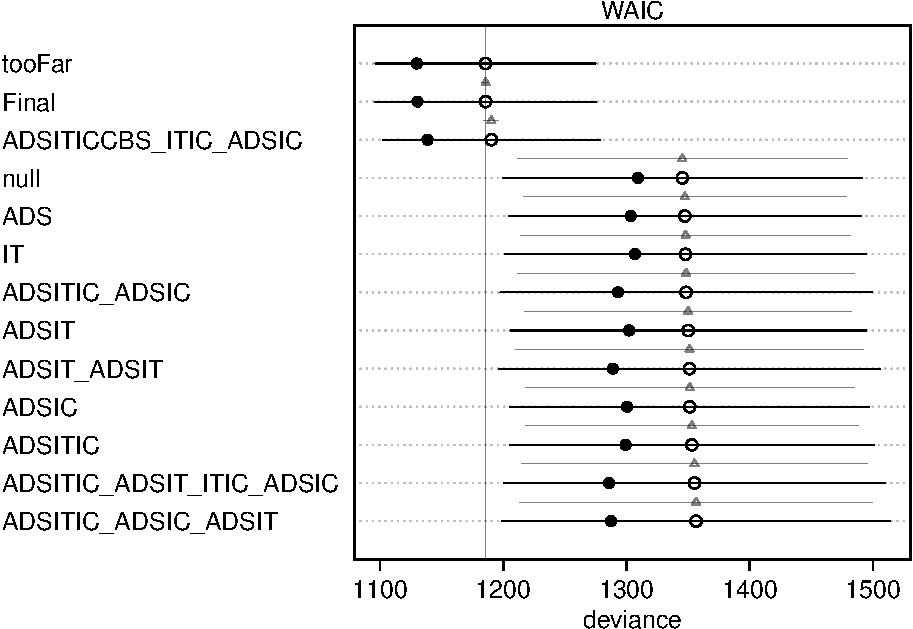
\includegraphics[width=1\linewidth]{bayesianReport3_files/figure-latex/unnamed-chunk-9-1} \end{center}

\normalsize

The three models that stand out differ in including \(\mathsf{CBS}\) as
a predictor. Moreover the final model includes an interaction between
treatment group and \(\mathsf{CBS}\). Adding a further interaction
between \(\mathsf{CBS}\) and \(\mathsf{IC}\) takes us too far.
\(WAIC\)-based weighing assigns the weight of \(83\%\) to the final
model, and the standard errors for the difference in WAIC for the top
three models is fairly low, so we will employ the top model
(\(\mathsf{Final}\)) in further analyses.

\section{Inspecting the model and effect
sizes}\label{inspecting-the-model-and-effect-sizes}

We start by using the \textsf{Final} model formula to build a model,
this time using Hamiltionian Monte Carlo. We leave the code commented
out and load a pre-compiled model for computational convenience

\vspace{1mm} \footnotesize

\begin{Shaded}
\begin{Highlighting}[]
\CommentTok{# FinalHMC <- ulam(}
\CommentTok{#   alist(}
\CommentTok{#     AdiffS ~ dnorm( mu, sigma ),}
\CommentTok{#     mu <- a + bADS[groupID] * ADS +  bIT[groupID] +}
\CommentTok{#     bIC[groupID] * IC + bADSIC * ADS * IC+}
\CommentTok{#     bCBS[groupID] *CBS,}
\CommentTok{#     a ~ dnorm (0,0.3),}
\CommentTok{#     bADS[groupID] ~ dnorm(0,.3),}
\CommentTok{#     bADSIC ~ dnorm(0,.3),}
\CommentTok{#     bCBS[groupID] ~ dnorm(0,.3),}
\CommentTok{#     bIT[groupID] ~ dnorm(0,.3),}
\CommentTok{#     bIC[groupID] ~ dnorm(0,.3),}
\CommentTok{#     sigma  ~ dexp(1)}
\CommentTok{#   ),}
\CommentTok{#   data = summaries}
\CommentTok{# )}
\CommentTok{# saveRDS(FinalHMC, file = "models/FinalHMC.rds")}


\CommentTok{#saveRDS(FinalHMC, file = "models/FinalHMC.rds")}

\NormalTok{FinalHMC <-}\StringTok{ }\KeywordTok{readRDS}\NormalTok{(}\DataTypeTok{file =} \StringTok{"models/FinalHMC.rds"}\NormalTok{)}
\end{Highlighting}
\end{Shaded}

\normalsize
First, let's take a look at the best model coefficients.

\vspace{1mm} \footnotesize

\begin{Shaded}
\begin{Highlighting}[]
\KeywordTok{mykable}\NormalTok{(}\KeywordTok{data.frame}\NormalTok{(}\KeywordTok{precis}\NormalTok{(FinalHMC, }\DataTypeTok{depth =} \DecValTok{2}\NormalTok{)))}
\end{Highlighting}
\end{Shaded}

\begin{table}
\centering\begingroup\fontsize{9}{11}\selectfont

\begin{tabular}{lrrrrrr}
\toprule
  & mean & sd & X5.5. & X94.5. & n\_eff & Rhat4\\
\midrule
\cellcolor{gray!6}{a} & \cellcolor{gray!6}{0.0414089} & \cellcolor{gray!6}{0.1562753} & \cellcolor{gray!6}{-0.2037740} & \cellcolor{gray!6}{0.2796946} & \cellcolor{gray!6}{228.1593} & \cellcolor{gray!6}{0.9980513}\\
bADS[1] & 0.1979211 & 0.0568494 & 0.1086423 & 0.2907669 & 768.4216 & 1.0013137\\
\cellcolor{gray!6}{bADS[2]} & \cellcolor{gray!6}{0.2484756} & \cellcolor{gray!6}{0.1546028} & \cellcolor{gray!6}{0.0036955} & \cellcolor{gray!6}{0.4942282} & \cellcolor{gray!6}{526.1494} & \cellcolor{gray!6}{0.9995921}\\
bADS[3] & -0.1097667 & 0.1014546 & -0.2678764 & 0.0628934 & 418.0876 & 0.9980791\\
\cellcolor{gray!6}{bADSIC} & \cellcolor{gray!6}{-0.0042060} & \cellcolor{gray!6}{0.0051643} & \cellcolor{gray!6}{-0.0122338} & \cellcolor{gray!6}{0.0040408} & \cellcolor{gray!6}{361.1195} & \cellcolor{gray!6}{0.9983620}\\
\addlinespace
bCBS[1] & -0.5142899 & 0.0414267 & -0.5776731 & -0.4463925 & 722.3116 & 0.9991926\\
\cellcolor{gray!6}{bCBS[2]} & \cellcolor{gray!6}{-0.0919148} & \cellcolor{gray!6}{0.1245614} & \cellcolor{gray!6}{-0.2965873} & \cellcolor{gray!6}{0.1059034} & \cellcolor{gray!6}{671.6673} & \cellcolor{gray!6}{0.9998084}\\
bCBS[3] & -0.5302840 & 0.1088835 & -0.7023272 & -0.3593766 & 823.7157 & 0.9980583\\
\cellcolor{gray!6}{bIT[1]} & \cellcolor{gray!6}{-0.0212337} & \cellcolor{gray!6}{0.1630179} & \cellcolor{gray!6}{-0.2603815} & \cellcolor{gray!6}{0.2295494} & \cellcolor{gray!6}{219.0190} & \cellcolor{gray!6}{0.9980137}\\
bIT[2] & 0.1482970 & 0.1857528 & -0.1246834 & 0.4367149 & 304.7859 & 0.9980345\\
\addlinespace
\cellcolor{gray!6}{bIT[3]} & \cellcolor{gray!6}{-0.0686005} & \cellcolor{gray!6}{0.1776783} & \cellcolor{gray!6}{-0.3448157} & \cellcolor{gray!6}{0.2099344} & \cellcolor{gray!6}{295.3412} & \cellcolor{gray!6}{0.9980482}\\
bIC[1] & -0.0037630 & 0.3161707 & -0.5084313 & 0.4981378 & 829.2326 & 1.0011451\\
\cellcolor{gray!6}{bIC[2]} & \cellcolor{gray!6}{-0.0117801} & \cellcolor{gray!6}{0.0256771} & \cellcolor{gray!6}{-0.0529960} & \cellcolor{gray!6}{0.0290304} & \cellcolor{gray!6}{488.1809} & \cellcolor{gray!6}{0.9994090}\\
bIC[3] & 0.0118155 & 0.0185521 & -0.0192521 & 0.0412303 & 612.3810 & 0.9986804\\
\cellcolor{gray!6}{sigma} & \cellcolor{gray!6}{0.7945882} & \cellcolor{gray!6}{0.0277774} & \cellcolor{gray!6}{0.7535960} & \cellcolor{gray!6}{0.8434971} & \cellcolor{gray!6}{693.5845} & \cellcolor{gray!6}{0.9982674}\\
\bottomrule
\end{tabular}
\endgroup{}
\end{table}

\begin{Shaded}
\begin{Highlighting}[]
\KeywordTok{plot}\NormalTok{(}\KeywordTok{precis}\NormalTok{(FinalHMC, }\DataTypeTok{depth =} \DecValTok{2}\NormalTok{))}
\end{Highlighting}
\end{Shaded}

\begin{center}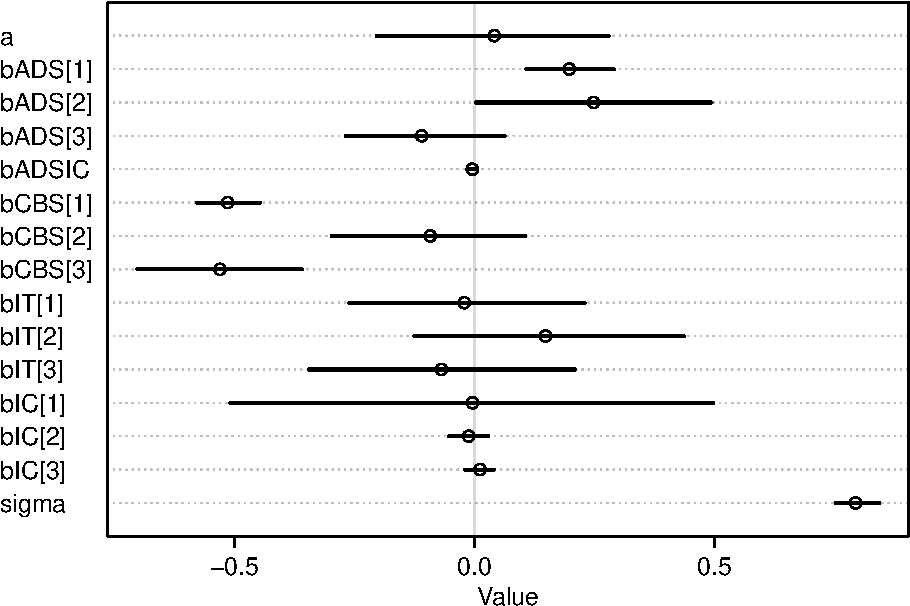
\includegraphics[width=1\linewidth]{bayesianReport3_files/figure-latex/unnamed-chunk-11-1} \end{center}

\normalsize

These, however, are notoriously hard to interpret in models with
interactions. For this reason, it is better to plot predicted effects
for various combinations of predictors.

\vspace{1mm} \footnotesize

\begin{Shaded}
\begin{Highlighting}[]
\NormalTok{visGroup <-}\StringTok{ }\ControlFlowTok{function}\NormalTok{ (model, ADS, CBS, }\DataTypeTok{xmin =}\DecValTok{2}\NormalTok{, }\DataTypeTok{ymax =} \DecValTok{-3}\NormalTok{)}
\NormalTok{\{}
\NormalTok{groupID <-}\StringTok{ }\DecValTok{1}\OperatorTok{:}\DecValTok{3}
\NormalTok{IC <-}\StringTok{ }\DecValTok{5} 
\NormalTok{data <-}\StringTok{ }\KeywordTok{expand.grid}\NormalTok{(}\DataTypeTok{ADS =}\NormalTok{ ADS,}\DataTypeTok{groupID =}\NormalTok{ groupID, }\DataTypeTok{CBS =}\NormalTok{ CBS, }\DataTypeTok{IC =}\NormalTok{  IC)}
\NormalTok{posterior <-}\StringTok{ }\KeywordTok{extract.samples}\NormalTok{(model, }\DataTypeTok{n =} \FloatTok{1e5}\NormalTok{)}
\NormalTok{mu <-}\StringTok{ }\KeywordTok{link}\NormalTok{( model, }\DataTypeTok{data=}\NormalTok{data ) }
\KeywordTok{colnames}\NormalTok{(mu) <-}\StringTok{ }\KeywordTok{levels}\NormalTok{(summaries}\OperatorTok{$}\NormalTok{group)}
\NormalTok{muLong <-}\StringTok{ }\KeywordTok{melt}\NormalTok{(mu)}
\KeywordTok{colnames}\NormalTok{(muLong) <-}\StringTok{ }\KeywordTok{c}\NormalTok{(}\StringTok{"id"}\NormalTok{, }\StringTok{"group"}\NormalTok{, }\StringTok{"AdiffS"}\NormalTok{)}
\NormalTok{means <-}\StringTok{  }\KeywordTok{round}\NormalTok{(}\KeywordTok{apply}\NormalTok{(mu , }\DecValTok{2}\NormalTok{ , mean ), }\DecValTok{2}\NormalTok{)}
\NormalTok{mu_HPDI <-}\StringTok{ }\KeywordTok{round}\NormalTok{(}\KeywordTok{apply}\NormalTok{( mu , }\DecValTok{2}\NormalTok{ , HPDI ),}\DecValTok{2}\NormalTok{)}
\NormalTok{means <-}\StringTok{ }\KeywordTok{as.data.frame}\NormalTok{(means)}
\NormalTok{means}\OperatorTok{$}\NormalTok{group <-}\StringTok{ }\KeywordTok{rownames}\NormalTok{(means)}
\KeywordTok{rownames}\NormalTok{(means) <-}\StringTok{ }\OtherTok{NULL}
\NormalTok{meansDisp <-}\StringTok{ }\KeywordTok{cbind}\NormalTok{(means,}\KeywordTok{t}\NormalTok{(}\KeywordTok{as.data.frame}\NormalTok{(mu_HPDI)))}
\NormalTok{meansDisp <-}\StringTok{ }\NormalTok{meansDisp[,}\KeywordTok{c}\NormalTok{(}\DecValTok{1}\NormalTok{,}\DecValTok{3}\NormalTok{,}\DecValTok{4}\NormalTok{)]}

\NormalTok{plot <-}\StringTok{ }\KeywordTok{ggplot}\NormalTok{(muLong)}\OperatorTok{+}\KeywordTok{geom_violin}\NormalTok{(}\KeywordTok{aes}\NormalTok{(}\DataTypeTok{x =}\NormalTok{ group, }\DataTypeTok{y =}\NormalTok{ AdiffS), }\DataTypeTok{alpha =} \FloatTok{0.2}\NormalTok{)}\OperatorTok{+}
\StringTok{  }\KeywordTok{xlab}\NormalTok{(}\StringTok{""}\NormalTok{)}\OperatorTok{+}
\StringTok{  }\KeywordTok{labs}\NormalTok{(}\DataTypeTok{title =} \KeywordTok{paste}\NormalTok{(}\StringTok{"ADS="}\NormalTok{, ADS, }\StringTok{", CBS="}\NormalTok{,  CBS,  }\DataTypeTok{sep =} \StringTok{""}\NormalTok{))}\OperatorTok{+}
\StringTok{  }\KeywordTok{theme_tufte}\NormalTok{()}\OperatorTok{+}\KeywordTok{ylim}\NormalTok{(}\KeywordTok{c}\NormalTok{(}\OperatorTok{-}\DecValTok{4}\NormalTok{,}\DecValTok{4}\NormalTok{))}
\CommentTok{#+   annotation_custom(tableGrob(meansDisp), xmin=xmin,  ymax=ymax)}
\KeywordTok{return}\NormalTok{(plot)}
\NormalTok{\}}


\NormalTok{visGroupA2C_}\DecValTok{2}\NormalTok{ <-}\StringTok{ }\KeywordTok{visGroup}\NormalTok{(}\DataTypeTok{model =}\NormalTok{ FinalHMC, }\DataTypeTok{ADS =} \DecValTok{2}\NormalTok{,}\DataTypeTok{CBS =} \DecValTok{-2}\NormalTok{)}
\NormalTok{visGroupA2C0 <-}\StringTok{ }\KeywordTok{visGroup}\NormalTok{(}\DataTypeTok{model =}\NormalTok{ FinalHMC, }\DataTypeTok{ADS =} \DecValTok{2}\NormalTok{,}\DataTypeTok{CBS =} \DecValTok{0}\NormalTok{ )}
\NormalTok{visGroupA2C2 <-}\StringTok{ }\KeywordTok{visGroup}\NormalTok{(}\DataTypeTok{model =}\NormalTok{ FinalHMC, }\DataTypeTok{ADS =} \DecValTok{2}\NormalTok{,}\DataTypeTok{CBS =} \DecValTok{2}\NormalTok{)}

\NormalTok{visGroupA0C_}\DecValTok{2}\NormalTok{ <-}\StringTok{ }\KeywordTok{visGroup}\NormalTok{(}\DataTypeTok{model =}\NormalTok{ FinalHMC, }\DataTypeTok{ADS =} \DecValTok{0}\NormalTok{,}\DataTypeTok{CBS =} \DecValTok{-2}\NormalTok{ )}
\NormalTok{visGroupA0C0 <-}\StringTok{ }\KeywordTok{visGroup}\NormalTok{(}\DataTypeTok{model =}\NormalTok{ FinalHMC, }\DataTypeTok{ADS =} \DecValTok{0}\NormalTok{,}\DataTypeTok{CBS =} \DecValTok{0}\NormalTok{ )}
\NormalTok{visGroupA0C2 <-}\StringTok{  }\KeywordTok{visGroup}\NormalTok{(}\DataTypeTok{model =}\NormalTok{ FinalHMC, }\DataTypeTok{ADS =} \DecValTok{0}\NormalTok{,}\DataTypeTok{CBS =} \DecValTok{2}\NormalTok{)}

\NormalTok{visGroupA2C_}\DecValTok{2}\NormalTok{ <-}\StringTok{  }\KeywordTok{visGroup}\NormalTok{(}\DataTypeTok{model =}\NormalTok{ FinalHMC, }\DataTypeTok{ADS =} \DecValTok{2}\NormalTok{,}\DataTypeTok{CBS =} \DecValTok{-2}\NormalTok{ )}
\NormalTok{visGroupA2C0 <-}\StringTok{ }\KeywordTok{visGroup}\NormalTok{(}\DataTypeTok{model =}\NormalTok{ FinalHMC, }\DataTypeTok{ADS =} \DecValTok{2}\NormalTok{,}\DataTypeTok{CBS =} \DecValTok{0}\NormalTok{ )}
\NormalTok{visGroupA2C2 <-}\StringTok{ }\KeywordTok{visGroup}\NormalTok{(}\DataTypeTok{model =}\NormalTok{ FinalHMC, }\DataTypeTok{ADS =} \DecValTok{2}\NormalTok{,}\DataTypeTok{CBS =} \DecValTok{2}\NormalTok{ )}

\NormalTok{visGroupJoint <-}\StringTok{ }\KeywordTok{ggarrange}\NormalTok{(visGroupA2C_}\DecValTok{2}\OperatorTok{+}\NormalTok{removeX }\OperatorTok{+}\StringTok{ }\KeywordTok{ggtitle}\NormalTok{(}\StringTok{"CBS = -2"}\NormalTok{)}\OperatorTok{+}\KeywordTok{ylab}\NormalTok{(}\StringTok{"ADS = 2"}\NormalTok{) , visGroupA2C0}\OperatorTok{+}\KeywordTok{theme_void}\NormalTok{()}\OperatorTok{+}\StringTok{ }\KeywordTok{ggtitle}\NormalTok{(}\StringTok{"CBS = 0"}\NormalTok{),visGroupA2C2}\OperatorTok{+}\KeywordTok{theme_void}\NormalTok{()}\OperatorTok{+}\StringTok{ }\KeywordTok{ggtitle}\NormalTok{(}\StringTok{"CBS = 2"}\NormalTok{), }
\NormalTok{          visGroupA0C_}\DecValTok{2}\OperatorTok{+}\NormalTok{removeX}\OperatorTok{+}\KeywordTok{ylab}\NormalTok{(}\StringTok{"ADS = 0"}\NormalTok{)}\OperatorTok{+}\KeywordTok{ggtitle}\NormalTok{(}\StringTok{""}\NormalTok{), visGroupA0C0}\OperatorTok{+}\KeywordTok{theme_void}\NormalTok{()}\OperatorTok{+}\KeywordTok{ggtitle}\NormalTok{(}\StringTok{""}\NormalTok{), visGroupA0C2}\OperatorTok{+}\KeywordTok{theme_void}\NormalTok{()}\OperatorTok{+}\KeywordTok{ggtitle}\NormalTok{(}\StringTok{""}\NormalTok{),}
\NormalTok{          visGroupA2C_}\DecValTok{2}\OperatorTok{+}\KeywordTok{ylab}\NormalTok{(}\StringTok{"ADS = -2"}\NormalTok{)}\OperatorTok{+}\KeywordTok{ggtitle}\NormalTok{(}\StringTok{""}\NormalTok{), visGroupA2C0}\OperatorTok{+}\NormalTok{removeY}\OperatorTok{+}\KeywordTok{ggtitle}\NormalTok{(}\StringTok{""}\NormalTok{), visGroupA2C2}\OperatorTok{+}\NormalTok{removeY}\OperatorTok{+}\KeywordTok{ggtitle}\NormalTok{(}\StringTok{""}\NormalTok{), }\DataTypeTok{ncol =}\DecValTok{3}\NormalTok{, }\DataTypeTok{nrow =} \DecValTok{3}\NormalTok{)}

 
\NormalTok{visGroupJoint2 <-}\StringTok{ }\KeywordTok{annotate_figure}\NormalTok{(visGroupJoint, }
  \DataTypeTok{top =} \KeywordTok{text_grob}\NormalTok{(}\StringTok{"(range restricted to (-4,4), IC at the rounded mean = 5)"}\NormalTok{,}
                  \DataTypeTok{size =} \DecValTok{10}\NormalTok{))}
\NormalTok{visGroupJoint3 <-}\StringTok{ }\KeywordTok{annotate_figure}\NormalTok{(visGroupJoint2, }
  \DataTypeTok{top =} \KeywordTok{text_grob}\NormalTok{(}\StringTok{"Predicted change in attacks by activity type and treatment groups (standardized)"}\NormalTok{,}
                  \DataTypeTok{size =} \DecValTok{12}\NormalTok{))}

\NormalTok{visGroupJoint3 }
\end{Highlighting}
\end{Shaded}

\begin{center}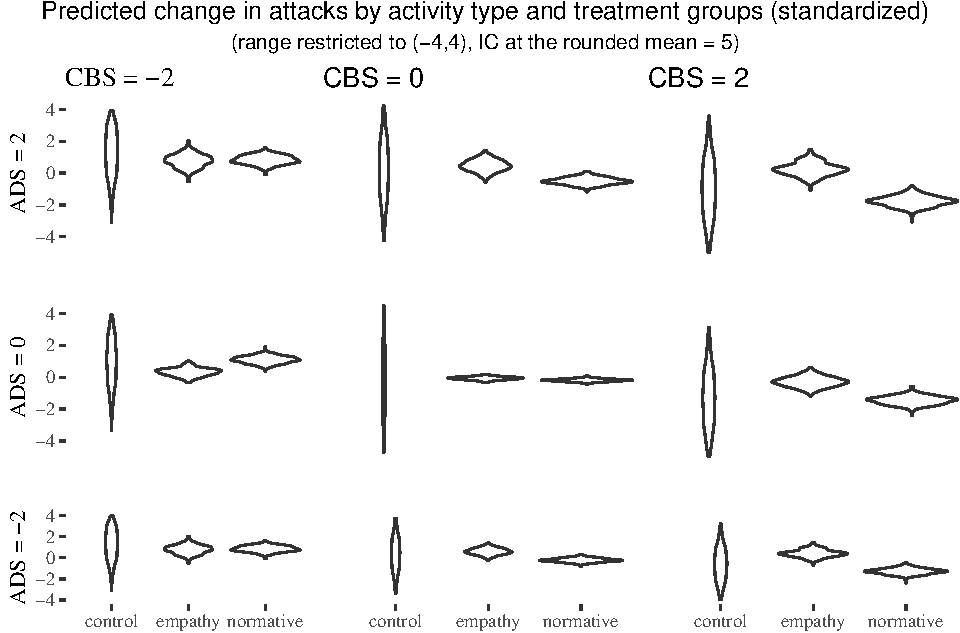
\includegraphics[width=1\linewidth]{bayesianReport3_files/figure-latex/unnamed-chunk-12-1} \end{center}

\normalsize

To gain more clarity, let's look at predicted contrasts, here understood
as distances from the control group mean, by activity types, first
versus CBS, then versus ADS.

\vspace{1mm} \footnotesize

\begin{Shaded}
\begin{Highlighting}[]
\NormalTok{visContrastsCBS <-}\StringTok{ }\ControlFlowTok{function}\NormalTok{(}\DataTypeTok{model =}\NormalTok{ FinalHMC, }\DataTypeTok{ADS =}\NormalTok{ ADS , }\DataTypeTok{IC =}  \DecValTok{5}\NormalTok{,}
                            \DataTypeTok{CBS =} \KeywordTok{seq}\NormalTok{(}\OperatorTok{-}\DecValTok{3}\NormalTok{,}\DecValTok{3}\NormalTok{,}\DataTypeTok{by  =} \FloatTok{0.1}\NormalTok{))}
\NormalTok{  \{}
\NormalTok{  groupID <-}\StringTok{ }\DecValTok{1}\OperatorTok{:}\DecValTok{3}
\NormalTok{  data <-}\StringTok{ }\KeywordTok{expand.grid}\NormalTok{(ADS, groupID, IC , CBS)}
  \KeywordTok{colnames}\NormalTok{(data) <-}\StringTok{ }\KeywordTok{c}\NormalTok{(}\StringTok{"ADS"}\NormalTok{, }\StringTok{"groupID"}\NormalTok{, }\StringTok{"IC"}\NormalTok{, }\StringTok{"CBS"}\NormalTok{)}
\NormalTok{  posterior <-}\StringTok{ }\KeywordTok{extract.samples}\NormalTok{(model, }\DataTypeTok{n =} \FloatTok{1e5}\NormalTok{)}
  \KeywordTok{link}\NormalTok{( model, }\DataTypeTok{data=}\NormalTok{data ) }
\NormalTok{  mu <-}\StringTok{ }\KeywordTok{link}\NormalTok{( model, }\DataTypeTok{data=}\NormalTok{data ) }
\NormalTok{  means <-}\StringTok{  }\KeywordTok{round}\NormalTok{(}\KeywordTok{apply}\NormalTok{(mu , }\DecValTok{2}\NormalTok{ , mean ), }\DecValTok{4}\NormalTok{)}
\NormalTok{  HPDIs <-}\StringTok{ }\KeywordTok{round}\NormalTok{(}\KeywordTok{apply}\NormalTok{( mu , }\DecValTok{2}\NormalTok{ , HPDI ),}\DecValTok{4}\NormalTok{)}
\NormalTok{  visContrast <-}\StringTok{ }\KeywordTok{cbind}\NormalTok{(data,means,}\KeywordTok{t}\NormalTok{(}\KeywordTok{as.data.frame}\NormalTok{(HPDIs)))}
  
\NormalTok{  ones <-}\StringTok{ }\DecValTok{3} \OperatorTok{*}\StringTok{ }\NormalTok{(}\DecValTok{1}\OperatorTok{:}\NormalTok{(}\KeywordTok{nrow}\NormalTok{(visContrast)}\OperatorTok{/}\DecValTok{3}\NormalTok{))}\OperatorTok{-}\DecValTok{2}
\NormalTok{  twos <-}\StringTok{ }\DecValTok{3} \OperatorTok{*}\StringTok{ }\NormalTok{(}\DecValTok{1}\OperatorTok{:}\NormalTok{(}\KeywordTok{nrow}\NormalTok{(visContrast)}\OperatorTok{/}\DecValTok{3}\NormalTok{))}\OperatorTok{-}\DecValTok{1}
\NormalTok{  threes <-}\StringTok{ }\DecValTok{3} \OperatorTok{*}\StringTok{ }\NormalTok{(}\DecValTok{1}\OperatorTok{:}\NormalTok{(}\KeywordTok{nrow}\NormalTok{(visContrast)}\OperatorTok{/}\DecValTok{3}\NormalTok{))}
  
  \KeywordTok{colnames}\NormalTok{(visContrast)[}\KeywordTok{c}\NormalTok{(}\DecValTok{6}\NormalTok{,}\DecValTok{7}\NormalTok{)] <-}\StringTok{ }\KeywordTok{c}\NormalTok{(}\StringTok{"low"}\NormalTok{, }\StringTok{"high"}\NormalTok{)}
\NormalTok{  contrast <-}\StringTok{ }\KeywordTok{numeric}\NormalTok{(}\KeywordTok{nrow}\NormalTok{(visContrast))}
\NormalTok{  cLow <-}\StringTok{ }\KeywordTok{numeric}\NormalTok{(}\KeywordTok{nrow}\NormalTok{(visContrast))}
\NormalTok{  cHigh <-}\StringTok{ }\KeywordTok{numeric}\NormalTok{(}\KeywordTok{nrow}\NormalTok{(visContrast))}
  \ControlFlowTok{for}\NormalTok{(i }\ControlFlowTok{in}\NormalTok{ threes)\{}
\NormalTok{  contrast[i] <-}\StringTok{ }\NormalTok{visContrast}\OperatorTok{$}\NormalTok{means[i] }\OperatorTok{-}\StringTok{ }\NormalTok{visContrast}\OperatorTok{$}\NormalTok{means[i}\DecValTok{-2}\NormalTok{]  }
\NormalTok{  \}}
  \ControlFlowTok{for}\NormalTok{(i }\ControlFlowTok{in}\NormalTok{ twos)\{}
\NormalTok{  contrast[i] <-}\StringTok{ }\NormalTok{visContrast}\OperatorTok{$}\NormalTok{means[i] }\OperatorTok{-}\StringTok{ }\NormalTok{visContrast}\OperatorTok{$}\NormalTok{means[i}\DecValTok{-1}\NormalTok{]  }
\NormalTok{  \}}
\NormalTok{  visContrast}\OperatorTok{$}\NormalTok{contrast <-}\StringTok{ }\NormalTok{contrast}
\NormalTok{  visContrast}\OperatorTok{$}\NormalTok{shift <-}\StringTok{  }\NormalTok{visContrast}\OperatorTok{$}\NormalTok{contrast }\OperatorTok{-}\StringTok{ }\NormalTok{visContrast}\OperatorTok{$}\NormalTok{means}
  \ControlFlowTok{for}\NormalTok{(i }\ControlFlowTok{in}\NormalTok{ ones)\{}
\NormalTok{  visContrast}\OperatorTok{$}\NormalTok{shift[i] <-}\StringTok{ }\DecValTok{0}
\NormalTok{  \}}
\NormalTok{  visContrast}\OperatorTok{$}\NormalTok{cLow <-}\StringTok{ }\NormalTok{visContrast}\OperatorTok{$}\NormalTok{low }\OperatorTok{+}\StringTok{ }\NormalTok{visContrast}\OperatorTok{$}\NormalTok{shift}
\NormalTok{  visContrast}\OperatorTok{$}\NormalTok{cHigh <-}\StringTok{ }\NormalTok{visContrast}\OperatorTok{$}\NormalTok{high }\OperatorTok{+}\StringTok{ }\NormalTok{visContrast}\OperatorTok{$}\NormalTok{shift}

\NormalTok{  visContrast}\OperatorTok{$}\NormalTok{group =}\StringTok{ }\KeywordTok{rep}\NormalTok{(}\KeywordTok{c}\NormalTok{(}\StringTok{"control"}\NormalTok{, }\StringTok{"empathy"}\NormalTok{, }\StringTok{"normative"}\NormalTok{), }
                          \KeywordTok{nrow}\NormalTok{(visContrast)}\OperatorTok{/}\DecValTok{3}\NormalTok{)}

\NormalTok{  visContrastTreatment <-}\StringTok{ }\NormalTok{visContrast[groupID }\OperatorTok{!=}\DecValTok{1}\NormalTok{,]}

  \KeywordTok{return}\NormalTok{(}\KeywordTok{ggplot}\NormalTok{(visContrastTreatment, }\KeywordTok{aes}\NormalTok{(}\DataTypeTok{x =}\NormalTok{ CBS, }\DataTypeTok{y =}\NormalTok{ contrast, }\DataTypeTok{fill =}\NormalTok{ group ))}\OperatorTok{+}
\StringTok{           }\KeywordTok{geom_line}\NormalTok{(}\DataTypeTok{se =} \OtherTok{FALSE}\NormalTok{)}\OperatorTok{+}
\StringTok{            }\KeywordTok{geom_ribbon}\NormalTok{(}\DataTypeTok{mapping =} 
        \KeywordTok{aes}\NormalTok{(}\DataTypeTok{ymin =}\NormalTok{ cLow, }\DataTypeTok{ymax =}\NormalTok{ cHigh),  }
         \DataTypeTok{alpha =} \FloatTok{.3}\NormalTok{)}\OperatorTok{+}
\StringTok{          }\KeywordTok{theme_tufte}\NormalTok{())}
\NormalTok{\}}


\NormalTok{visContrastCBSJoint <-}\StringTok{ }\KeywordTok{ggarrange}\NormalTok{(}\KeywordTok{visContrastsCBS}\NormalTok{(FinalHMC,}\DataTypeTok{ADS =} \DecValTok{-2}\NormalTok{)}\OperatorTok{+}
\StringTok{      }\KeywordTok{ggtitle}\NormalTok{(}\StringTok{"ADS = -2"}\NormalTok{)}\OperatorTok{+}\KeywordTok{ylim}\NormalTok{(}\KeywordTok{c}\NormalTok{(}\OperatorTok{-}\FloatTok{2.5}\NormalTok{,}\FloatTok{2.5}\NormalTok{))}\OperatorTok{+}\StringTok{ }\KeywordTok{scale_fill_discrete}\NormalTok{(}\DataTypeTok{guide=}\OtherTok{FALSE}\NormalTok{),}
          \KeywordTok{visContrastsCBS}\NormalTok{(FinalHMC,}\DataTypeTok{ADS =} \DecValTok{0}\NormalTok{)}\OperatorTok{+}\KeywordTok{ggtitle}\NormalTok{(}\StringTok{"ADS = 0"}\NormalTok{)}\OperatorTok{+}
\StringTok{        }\KeywordTok{ylim}\NormalTok{(}\KeywordTok{c}\NormalTok{(}\OperatorTok{-}\FloatTok{2.5}\NormalTok{,}\FloatTok{2.5}\NormalTok{))}\OperatorTok{+}\StringTok{ }\KeywordTok{scale_fill_discrete}\NormalTok{(}\DataTypeTok{guide=}\OtherTok{FALSE}\NormalTok{)}\OperatorTok{+}
\StringTok{        }\NormalTok{removeY,}
        \KeywordTok{visContrastsCBS}\NormalTok{(FinalHMC,}\DataTypeTok{ADS =} \DecValTok{2}\NormalTok{)}\OperatorTok{+}\KeywordTok{ggtitle}\NormalTok{(}\StringTok{"ADS = 2"}\NormalTok{)}\OperatorTok{+}
\StringTok{        }\KeywordTok{ylim}\NormalTok{(}\KeywordTok{c}\NormalTok{(}\OperatorTok{-}\FloatTok{2.5}\NormalTok{,}\FloatTok{2.5}\NormalTok{))}\OperatorTok{+}\StringTok{ }\KeywordTok{theme}\NormalTok{(}\DataTypeTok{legend.position =} \KeywordTok{c}\NormalTok{(}\FloatTok{0.75}\NormalTok{, }\FloatTok{0.15}\NormalTok{))}\OperatorTok{+}
\StringTok{        }\NormalTok{removeY, }\DataTypeTok{ncol =} \DecValTok{3}\NormalTok{)}

\NormalTok{visContrastCBSJoint2 <-}\StringTok{ }\KeywordTok{annotate_figure}\NormalTok{(visContrastCBSJoint, }
      \DataTypeTok{top =} \KeywordTok{text_grob}\NormalTok{(}\StringTok{"(range restricted to (-2.5,2.5), IC at the rounded mean = 5)"}\NormalTok{,}
                                \DataTypeTok{size =} \DecValTok{10}\NormalTok{))}
\NormalTok{visContrastCBSJoint3 <-}\StringTok{ }\KeywordTok{annotate_figure}\NormalTok{(visContrastCBSJoint2, }
\DataTypeTok{top =} \KeywordTok{text_grob}\NormalTok{(}\StringTok{"Predicted distance from the control group mean vs. CBS  (standardized)"}\NormalTok{,}
                                \DataTypeTok{size =} \DecValTok{12}\NormalTok{))}

\NormalTok{visContrastCBSJoint3}
\end{Highlighting}
\end{Shaded}

\begin{center}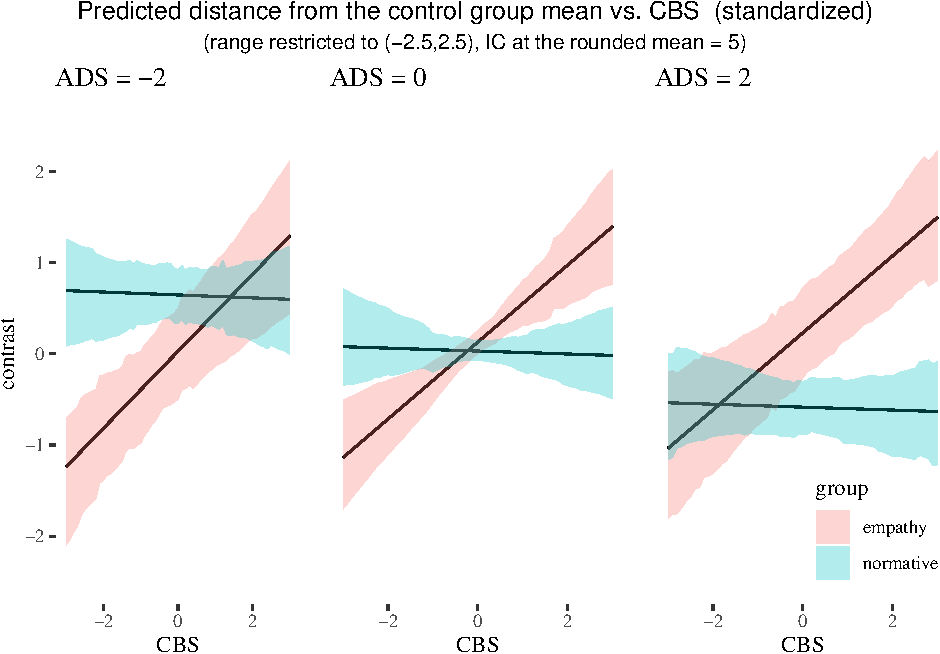
\includegraphics[width=1\linewidth]{bayesianReport3_files/figure-latex/unnamed-chunk-13-1} \end{center}

\normalsize

\vspace{1mm} \footnotesize

\begin{Shaded}
\begin{Highlighting}[]
\NormalTok{visContrastsADS <-}\StringTok{ }\ControlFlowTok{function}\NormalTok{(}\DataTypeTok{model =}\NormalTok{ FinalHMC, }\DataTypeTok{CBS =}\NormalTok{ CBS , }\DataTypeTok{IC =}  \DecValTok{5}\NormalTok{, }
                            \DataTypeTok{ADS =} \KeywordTok{seq}\NormalTok{(}\OperatorTok{-}\DecValTok{3}\NormalTok{,}\DecValTok{3}\NormalTok{,}\DataTypeTok{by  =} \FloatTok{0.1}\NormalTok{))}
\NormalTok{\{}
\NormalTok{  data <-}\StringTok{ }\KeywordTok{expand.grid}\NormalTok{(CBS, groupID, IC , ADS)}
  \KeywordTok{colnames}\NormalTok{(data) <-}\StringTok{ }\KeywordTok{c}\NormalTok{(}\StringTok{"CBS"}\NormalTok{, }\StringTok{"groupID"}\NormalTok{, }\StringTok{"IC"}\NormalTok{, }\StringTok{"ADS"}\NormalTok{)}
\NormalTok{  posterior <-}\StringTok{ }\KeywordTok{extract.samples}\NormalTok{(model, }\DataTypeTok{n =} \FloatTok{1e5}\NormalTok{)}
\NormalTok{  mu <-}\StringTok{ }\KeywordTok{link}\NormalTok{( model, }\DataTypeTok{data=}\NormalTok{data ) }
\NormalTok{  means <-}\StringTok{  }\KeywordTok{round}\NormalTok{(}\KeywordTok{apply}\NormalTok{(mu , }\DecValTok{2}\NormalTok{ , mean ), }\DecValTok{4}\NormalTok{)}
\NormalTok{  HPDIs <-}\StringTok{ }\KeywordTok{round}\NormalTok{(}\KeywordTok{apply}\NormalTok{( mu , }\DecValTok{2}\NormalTok{ , HPDI ),}\DecValTok{4}\NormalTok{)}
\NormalTok{  visContrastADS <-}\StringTok{ }\KeywordTok{cbind}\NormalTok{(data,means,}\KeywordTok{t}\NormalTok{(}\KeywordTok{as.data.frame}\NormalTok{(HPDIs)))}


\NormalTok{  ones <-}\StringTok{ }\DecValTok{3} \OperatorTok{*}\StringTok{ }\NormalTok{(}\DecValTok{1}\OperatorTok{:}\NormalTok{(}\KeywordTok{nrow}\NormalTok{(visContrastADS)}\OperatorTok{/}\DecValTok{3}\NormalTok{))}\OperatorTok{-}\DecValTok{2}
\NormalTok{  twos <-}\StringTok{ }\DecValTok{3} \OperatorTok{*}\StringTok{ }\NormalTok{(}\DecValTok{1}\OperatorTok{:}\NormalTok{(}\KeywordTok{nrow}\NormalTok{(visContrastADS)}\OperatorTok{/}\DecValTok{3}\NormalTok{))}\OperatorTok{-}\DecValTok{1}
\NormalTok{  threes <-}\StringTok{ }\DecValTok{3} \OperatorTok{*}\StringTok{ }\NormalTok{(}\DecValTok{1}\OperatorTok{:}\NormalTok{(}\KeywordTok{nrow}\NormalTok{(visContrastADS)}\OperatorTok{/}\DecValTok{3}\NormalTok{))}
  
  \KeywordTok{colnames}\NormalTok{(visContrastADS)[}\KeywordTok{c}\NormalTok{(}\DecValTok{6}\NormalTok{,}\DecValTok{7}\NormalTok{)] <-}\StringTok{ }\KeywordTok{c}\NormalTok{(}\StringTok{"low"}\NormalTok{, }\StringTok{"high"}\NormalTok{)}
\NormalTok{  contrastADS <-}\StringTok{ }\KeywordTok{numeric}\NormalTok{(}\KeywordTok{nrow}\NormalTok{(visContrastADS))}
  \ControlFlowTok{for}\NormalTok{(i }\ControlFlowTok{in}\NormalTok{ threes)\{}
\NormalTok{    contrastADS[i] <-}\StringTok{ }\NormalTok{visContrastADS}\OperatorTok{$}\NormalTok{means[i] }\OperatorTok{-}\StringTok{ }\NormalTok{visContrastADS}\OperatorTok{$}\NormalTok{means[i}\DecValTok{-2}\NormalTok{]  }
\NormalTok{  \}}
  \ControlFlowTok{for}\NormalTok{(i }\ControlFlowTok{in}\NormalTok{ twos)\{}
\NormalTok{    contrastADS[i] <-}\StringTok{ }\NormalTok{visContrastADS}\OperatorTok{$}\NormalTok{means[i] }\OperatorTok{-}\StringTok{ }\NormalTok{visContrastADS}\OperatorTok{$}\NormalTok{means[i}\DecValTok{-1}\NormalTok{]  }
\NormalTok{  \}}
\NormalTok{  visContrastADS}\OperatorTok{$}\NormalTok{contrast <-}\StringTok{ }\NormalTok{contrastADS}
\NormalTok{  visContrastADS}\OperatorTok{$}\NormalTok{shift <-}\StringTok{  }\NormalTok{visContrastADS}\OperatorTok{$}\NormalTok{contrast }\OperatorTok{-}\StringTok{ }\NormalTok{visContrastADS}\OperatorTok{$}\NormalTok{means}
  \ControlFlowTok{for}\NormalTok{(i }\ControlFlowTok{in}\NormalTok{ ones)\{}
\NormalTok{    visContrastADS}\OperatorTok{$}\NormalTok{shift[i] <-}\StringTok{ }\DecValTok{0}
\NormalTok{  \}}
\NormalTok{  visContrastADS}\OperatorTok{$}\NormalTok{cLow <-}\StringTok{ }\NormalTok{visContrastADS}\OperatorTok{$}\NormalTok{low }\OperatorTok{+}\StringTok{ }\NormalTok{visContrastADS}\OperatorTok{$}\NormalTok{shift}
\NormalTok{  visContrastADS}\OperatorTok{$}\NormalTok{cHigh <-}\StringTok{ }\NormalTok{visContrastADS}\OperatorTok{$}\NormalTok{high }\OperatorTok{+}\StringTok{ }\NormalTok{visContrastADS}\OperatorTok{$}\NormalTok{shift}
  
\NormalTok{  visContrastADS}\OperatorTok{$}\NormalTok{group =}\StringTok{ }\KeywordTok{rep}\NormalTok{(}\KeywordTok{c}\NormalTok{(}\StringTok{"control"}\NormalTok{, }\StringTok{"empathy"}\NormalTok{, }\StringTok{"normative"}\NormalTok{), }
                             \KeywordTok{nrow}\NormalTok{(visContrastADS)}\OperatorTok{/}\DecValTok{3}\NormalTok{)}
\NormalTok{  visContrastTreatmentADS <-}\StringTok{ }\NormalTok{visContrastADS[groupID }\OperatorTok{!=}\DecValTok{1}\NormalTok{,]}

  \KeywordTok{return}\NormalTok{(}\KeywordTok{ggplot}\NormalTok{(visContrastTreatmentADS, }\KeywordTok{aes}\NormalTok{(}\DataTypeTok{x =}\NormalTok{ ADS, }\DataTypeTok{y =}\NormalTok{ contrast, }\DataTypeTok{fill =}\NormalTok{ group ))}\OperatorTok{+}
\StringTok{           }\KeywordTok{geom_line}\NormalTok{(}\DataTypeTok{se =} \OtherTok{FALSE}\NormalTok{) }\OperatorTok{+}
\StringTok{  }\KeywordTok{geom_ribbon}\NormalTok{(}\DataTypeTok{mapping =} \KeywordTok{aes}\NormalTok{(}\DataTypeTok{ymin =}\NormalTok{ cLow, }\DataTypeTok{ymax =}\NormalTok{ cHigh), }
       \DataTypeTok{alpha =} \FloatTok{.3}\NormalTok{) }\OperatorTok{+}\KeywordTok{theme_tufte}\NormalTok{())}
\NormalTok{\}}



\NormalTok{visContrastADSJoint <-}\StringTok{ }\KeywordTok{ggarrange}\NormalTok{(}\KeywordTok{visContrastsADS}\NormalTok{(FinalHMC,}\DataTypeTok{CBS =} \DecValTok{-2}\NormalTok{)}\OperatorTok{+}\KeywordTok{ggtitle}\NormalTok{(}\StringTok{"CBS = -2"}\NormalTok{)}
                                 \OperatorTok{+}\KeywordTok{ylim}\NormalTok{(}\KeywordTok{c}\NormalTok{(}\OperatorTok{-}\FloatTok{2.5}\NormalTok{,}\FloatTok{2.5}\NormalTok{))}\OperatorTok{+}\StringTok{ }\KeywordTok{scale_fill_discrete}\NormalTok{(}\DataTypeTok{guide=}\OtherTok{FALSE}\NormalTok{),}
                                 \KeywordTok{visContrastsADS}\NormalTok{(FinalHMC,}\DataTypeTok{CBS =} \DecValTok{0}\NormalTok{)}\OperatorTok{+}\KeywordTok{ggtitle}\NormalTok{(}\StringTok{"CBS = 0"}\NormalTok{)}
                                 \OperatorTok{+}\KeywordTok{ylim}\NormalTok{(}\KeywordTok{c}\NormalTok{(}\OperatorTok{-}\FloatTok{2.5}\NormalTok{,}\FloatTok{2.5}\NormalTok{))}\OperatorTok{+}\StringTok{ }\KeywordTok{scale_fill_discrete}\NormalTok{(}\DataTypeTok{guide=}\OtherTok{FALSE}\NormalTok{)}\OperatorTok{+}
\StringTok{                                   }\NormalTok{removeY,}
                                 \KeywordTok{visContrastsADS}\NormalTok{(FinalHMC,}\DataTypeTok{CBS =} \DecValTok{2}\NormalTok{)}\OperatorTok{+}\KeywordTok{ggtitle}\NormalTok{(}\StringTok{"CBS = 2"}\NormalTok{)}
                                 \OperatorTok{+}\KeywordTok{ylim}\NormalTok{(}\KeywordTok{c}\NormalTok{(}\OperatorTok{-}\FloatTok{2.5}\NormalTok{,}\FloatTok{2.5}\NormalTok{))}\OperatorTok{+}
\StringTok{                                   }\KeywordTok{theme}\NormalTok{(}\DataTypeTok{legend.position =} \KeywordTok{c}\NormalTok{(}\FloatTok{0.75}\NormalTok{, }\FloatTok{0.15}\NormalTok{))}\OperatorTok{+}
\StringTok{                                   }\NormalTok{removeY, }\DataTypeTok{ncol =} \DecValTok{3}\NormalTok{)}

\NormalTok{visContrastADSJoint2 <-}\StringTok{ }\KeywordTok{annotate_figure}\NormalTok{(visContrastADSJoint, }
\DataTypeTok{top =} \KeywordTok{text_grob}\NormalTok{(}\StringTok{"(range restricted to (-2.5,2.5), IC at the rounded mean = 5)"}\NormalTok{,}
                                                        \DataTypeTok{size =} \DecValTok{10}\NormalTok{))}
\NormalTok{visContrastADSJoint3 <-}\StringTok{ }\KeywordTok{annotate_figure}\NormalTok{(visContrastADSJoint2, }
\DataTypeTok{top =} \KeywordTok{text_grob}\NormalTok{(}\StringTok{"Predicted distance from the control group mean vs. ADS (standardized)"}\NormalTok{,}
                                                        \DataTypeTok{size =} \DecValTok{12}\NormalTok{))}

\NormalTok{visContrastADSJoint3}
\end{Highlighting}
\end{Shaded}

\begin{center}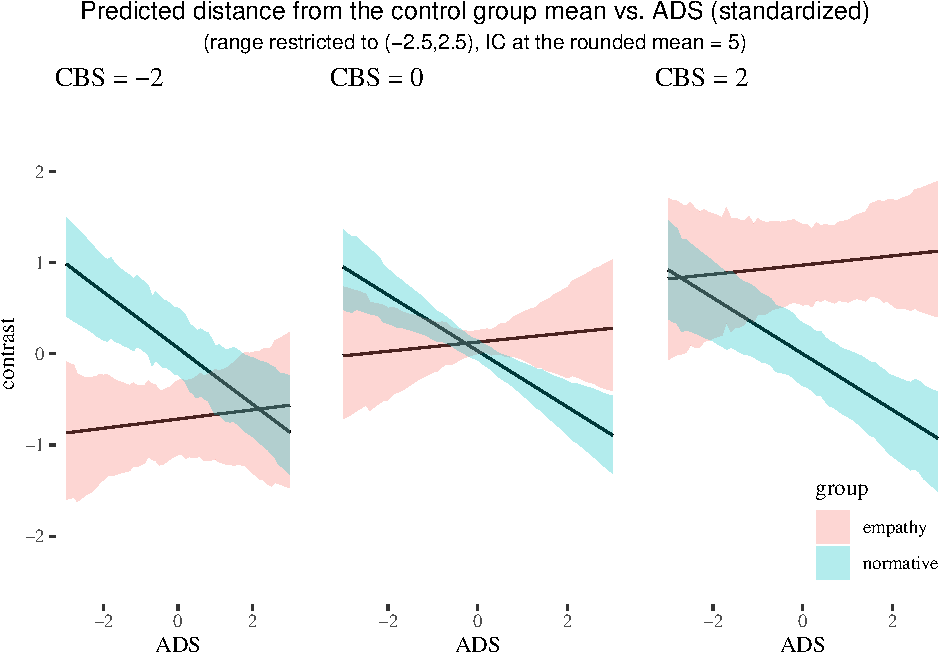
\includegraphics[width=1\linewidth]{bayesianReport3_files/figure-latex/unnamed-chunk-14-1} \end{center}

\normalsize

Now, let's inspect the impact of intervention counts by treatment type
by looking at contrasts (distances from the control group mean) with
89\% HPDIs by IC. Notice the predicted effect of \textsf{IC} is weaker
than group membership, so for visibility the \(y\)-axis has a smaller
range. Also, not enough data was available to reliably estimate
uncertainty for \textsf{IC} above 20, hence the restriction on the
\(x\)-axis (arleady at lower values, lack of estimates is visible for
the more extreme covariate settings).

\vspace{1mm} \footnotesize

\begin{Shaded}
\begin{Highlighting}[]
\NormalTok{visContrastsIC <-}\StringTok{ }\ControlFlowTok{function}\NormalTok{(}\DataTypeTok{model =}\NormalTok{ FinalHMC, }\DataTypeTok{CBS =}\NormalTok{ CBS ,}
                           \DataTypeTok{IC =}  \KeywordTok{seq}\NormalTok{(}\DecValTok{0}\NormalTok{,}\DecValTok{20}\NormalTok{,}\DataTypeTok{by =} \DecValTok{1}\NormalTok{), }\DataTypeTok{ADS =}\NormalTok{ ADS)}
\NormalTok{\{}
\NormalTok{  groupID <-}\StringTok{ }\DecValTok{1}\OperatorTok{:}\DecValTok{3}
\NormalTok{  data <-}\StringTok{ }\KeywordTok{expand.grid}\NormalTok{(CBS, groupID, IC , ADS)}
\NormalTok{  data}
  \KeywordTok{colnames}\NormalTok{(data) <-}\StringTok{ }\KeywordTok{c}\NormalTok{(}\StringTok{"CBS"}\NormalTok{, }\StringTok{"groupID"}\NormalTok{, }\StringTok{"IC"}\NormalTok{, }\StringTok{"ADS"}\NormalTok{)}
\NormalTok{  posterior <-}\StringTok{ }\KeywordTok{extract.samples}\NormalTok{(model, }\DataTypeTok{n =} \FloatTok{1e5}\NormalTok{)}
\NormalTok{  mu <-}\StringTok{ }\KeywordTok{link}\NormalTok{( model, }\DataTypeTok{data=}\NormalTok{data ) }
\NormalTok{  means <-}\StringTok{  }\KeywordTok{round}\NormalTok{(}\KeywordTok{apply}\NormalTok{(mu , }\DecValTok{2}\NormalTok{ , mean ), }\DecValTok{4}\NormalTok{)}
\NormalTok{  HPDIs <-}\StringTok{ }\KeywordTok{round}\NormalTok{(}\KeywordTok{apply}\NormalTok{( mu , }\DecValTok{2}\NormalTok{ , HPDI ),}\DecValTok{4}\NormalTok{)}
\NormalTok{  visContrastIC <-}\StringTok{ }\KeywordTok{cbind}\NormalTok{(data,means,}\KeywordTok{t}\NormalTok{(}\KeywordTok{as.data.frame}\NormalTok{(HPDIs)))}
  
\NormalTok{  ones <-}\StringTok{ }\DecValTok{3} \OperatorTok{*}\StringTok{ }\NormalTok{(}\DecValTok{1}\OperatorTok{:}\NormalTok{(}\KeywordTok{nrow}\NormalTok{(visContrastIC)}\OperatorTok{/}\DecValTok{3}\NormalTok{))}\OperatorTok{-}\DecValTok{2}
\NormalTok{  twos <-}\StringTok{ }\DecValTok{3} \OperatorTok{*}\StringTok{ }\NormalTok{(}\DecValTok{1}\OperatorTok{:}\NormalTok{(}\KeywordTok{nrow}\NormalTok{(visContrastIC)}\OperatorTok{/}\DecValTok{3}\NormalTok{))}\OperatorTok{-}\DecValTok{1}
\NormalTok{  threes <-}\StringTok{ }\DecValTok{3} \OperatorTok{*}\StringTok{ }\NormalTok{(}\DecValTok{1}\OperatorTok{:}\NormalTok{(}\KeywordTok{nrow}\NormalTok{(visContrastIC)}\OperatorTok{/}\DecValTok{3}\NormalTok{))}
  
  \KeywordTok{colnames}\NormalTok{(visContrastIC)[}\KeywordTok{c}\NormalTok{(}\DecValTok{6}\NormalTok{,}\DecValTok{7}\NormalTok{)] <-}\StringTok{ }\KeywordTok{c}\NormalTok{(}\StringTok{"low"}\NormalTok{, }\StringTok{"high"}\NormalTok{)}
\NormalTok{  contrastIC <-}\StringTok{ }\KeywordTok{numeric}\NormalTok{(}\KeywordTok{nrow}\NormalTok{(visContrastIC))}
  \ControlFlowTok{for}\NormalTok{(i }\ControlFlowTok{in}\NormalTok{ threes)\{}
\NormalTok{    contrastIC[i] <-}\StringTok{ }\NormalTok{visContrastIC}\OperatorTok{$}\NormalTok{means[i] }\OperatorTok{-}\StringTok{ }\NormalTok{visContrastIC}\OperatorTok{$}\NormalTok{means[i}\DecValTok{-2}\NormalTok{]  }
\NormalTok{  \}}
  \ControlFlowTok{for}\NormalTok{(i }\ControlFlowTok{in}\NormalTok{ twos)\{}
\NormalTok{    contrastIC[i] <-}\StringTok{ }\NormalTok{visContrastIC}\OperatorTok{$}\NormalTok{means[i] }\OperatorTok{-}\StringTok{ }\NormalTok{visContrastIC}\OperatorTok{$}\NormalTok{means[i}\DecValTok{-1}\NormalTok{]  }
\NormalTok{  \}}
\NormalTok{  visContrastIC}\OperatorTok{$}\NormalTok{contrast <-}\StringTok{ }\NormalTok{contrastIC}
\NormalTok{  visContrastIC}\OperatorTok{$}\NormalTok{shift <-}\StringTok{  }\NormalTok{visContrastIC}\OperatorTok{$}\NormalTok{contrast }\OperatorTok{-}\StringTok{ }\NormalTok{visContrastIC}\OperatorTok{$}\NormalTok{means}
  \ControlFlowTok{for}\NormalTok{(i }\ControlFlowTok{in}\NormalTok{ ones)\{}
\NormalTok{    visContrastIC}\OperatorTok{$}\NormalTok{shift[i] <-}\StringTok{ }\DecValTok{0}
\NormalTok{  \}}
\NormalTok{  visContrastIC}\OperatorTok{$}\NormalTok{cLow <-}\StringTok{ }\NormalTok{visContrastIC}\OperatorTok{$}\NormalTok{low }\OperatorTok{+}\StringTok{ }\NormalTok{visContrastIC}\OperatorTok{$}\NormalTok{shift}
\NormalTok{  visContrastIC}\OperatorTok{$}\NormalTok{cHigh <-}\StringTok{ }\NormalTok{visContrastIC}\OperatorTok{$}\NormalTok{high }\OperatorTok{+}\StringTok{ }\NormalTok{visContrastIC}\OperatorTok{$}\NormalTok{shift}
  
\NormalTok{  visContrastIC}\OperatorTok{$}\NormalTok{group =}\StringTok{ }\KeywordTok{rep}\NormalTok{(}\KeywordTok{c}\NormalTok{(}\StringTok{"control"}\NormalTok{, }\StringTok{"empathy"}\NormalTok{, }\StringTok{"normative"}\NormalTok{),}
                            \KeywordTok{nrow}\NormalTok{(visContrastIC)}\OperatorTok{/}\DecValTok{3}\NormalTok{)}
\NormalTok{  visContrastTreatmentIC <-}\StringTok{ }\NormalTok{visContrastIC[groupID }\OperatorTok{!=}\DecValTok{1}\NormalTok{,]}
  
  \KeywordTok{return}\NormalTok{(}\KeywordTok{ggplot}\NormalTok{(visContrastTreatmentIC, }\KeywordTok{aes}\NormalTok{(}\DataTypeTok{x =}\NormalTok{ IC, }\DataTypeTok{y =}\NormalTok{ contrast, }\DataTypeTok{fill =}\NormalTok{ group ))}\OperatorTok{+}
\StringTok{           }\KeywordTok{geom_line}\NormalTok{(}\DataTypeTok{se=}\OtherTok{FALSE}\NormalTok{)}\OperatorTok{+}
\StringTok{    }\KeywordTok{geom_ribbon}\NormalTok{(}\DataTypeTok{mapping =} \KeywordTok{aes}\NormalTok{(}\DataTypeTok{ymin =}\NormalTok{ cLow, }\DataTypeTok{ymax =}\NormalTok{ cHigh), }\DataTypeTok{alpha =} \FloatTok{.3}\NormalTok{)}\OperatorTok{+}
\StringTok{    }\KeywordTok{ylim}\NormalTok{(}\KeywordTok{c}\NormalTok{(}\OperatorTok{-}\DecValTok{2}\NormalTok{,}\DecValTok{2}\NormalTok{)) }\OperatorTok{+}\KeywordTok{theme_tufte}\NormalTok{()}\OperatorTok{+}\KeywordTok{geom_hline}\NormalTok{(}\DataTypeTok{yintercept =} \DecValTok{0}\NormalTok{, }\DataTypeTok{lty =}\DecValTok{2}\NormalTok{, }\DataTypeTok{size =} \FloatTok{0.1}\NormalTok{))}
\NormalTok{\}}


\NormalTok{visContrastsICJoint <-}\StringTok{ }\KeywordTok{ggarrange}\NormalTok{(}
\KeywordTok{visContrastsIC}\NormalTok{(}\DataTypeTok{ADS =} \DecValTok{2}\NormalTok{, }\DataTypeTok{CBS =} \DecValTok{-2}\NormalTok{)}\OperatorTok{+}\NormalTok{removeX}\OperatorTok{+}\StringTok{ }
\StringTok{               }\KeywordTok{theme}\NormalTok{(}\DataTypeTok{legend.position =} \KeywordTok{c}\NormalTok{(}\FloatTok{0.3}\NormalTok{, }\FloatTok{0.9}\NormalTok{),}
                     \DataTypeTok{legend.key.size =} \KeywordTok{unit}\NormalTok{(.}\DecValTok{3}\NormalTok{, }\StringTok{'cm'}\NormalTok{),}
                     \DataTypeTok{legend.key.height =} \KeywordTok{unit}\NormalTok{(.}\DecValTok{3}\NormalTok{, }\StringTok{'cm'}\NormalTok{),}
                     \DataTypeTok{legend.key.width =} \KeywordTok{unit}\NormalTok{(.}\DecValTok{3}\NormalTok{, }\StringTok{'cm'}\NormalTok{),}
                     \DataTypeTok{legend.title=} \KeywordTok{element_blank}\NormalTok{())}\OperatorTok{+}
\StringTok{  }\KeywordTok{ggtitle}\NormalTok{(}\StringTok{"CBS = -2"}\NormalTok{)}\OperatorTok{+}
\StringTok{  }\KeywordTok{ylab}\NormalTok{(}\StringTok{"ADS = 2"}\NormalTok{),}
    \KeywordTok{visContrastsIC}\NormalTok{(}\DataTypeTok{ADS =} \DecValTok{2}\NormalTok{, }\DataTypeTok{CBS =} \DecValTok{0}\NormalTok{)}\OperatorTok{+}\NormalTok{removeY}\OperatorTok{+}\NormalTok{removeX}\OperatorTok{+}\StringTok{ }\KeywordTok{scale_fill_discrete}\NormalTok{(}\DataTypeTok{guide=}\OtherTok{FALSE}\NormalTok{)}\OperatorTok{+}
\StringTok{  }\KeywordTok{ggtitle}\NormalTok{(}\StringTok{"CBS = 0"}\NormalTok{),}
    \KeywordTok{visContrastsIC}\NormalTok{(}\DataTypeTok{ADS =} \DecValTok{2}\NormalTok{, }\DataTypeTok{CBS =} \DecValTok{2}\NormalTok{)}\OperatorTok{+}\NormalTok{removeY}\OperatorTok{+}\NormalTok{removeX}\OperatorTok{+}\KeywordTok{ggtitle}\NormalTok{(}\StringTok{"CBS = 2"}\NormalTok{)}\OperatorTok{+}\StringTok{ }\KeywordTok{scale_fill_discrete}\NormalTok{(}\DataTypeTok{guide=}\OtherTok{FALSE}\NormalTok{),}
\KeywordTok{visContrastsIC}\NormalTok{(}\DataTypeTok{ADS =} \DecValTok{0}\NormalTok{, }\DataTypeTok{CBS =} \DecValTok{-2}\NormalTok{)}\OperatorTok{+}\NormalTok{removeX}\OperatorTok{+}\StringTok{ }\KeywordTok{scale_fill_discrete}\NormalTok{(}\DataTypeTok{guide=}\OtherTok{FALSE}\NormalTok{)}\OperatorTok{+}
\StringTok{  }\KeywordTok{ylab}\NormalTok{(}\StringTok{"ADS = 0"}\NormalTok{),}
    \KeywordTok{visContrastsIC}\NormalTok{(}\DataTypeTok{ADS =} \DecValTok{0}\NormalTok{, }\DataTypeTok{CBS =} \DecValTok{0}\NormalTok{)}\OperatorTok{+}\NormalTok{removeY}\OperatorTok{+}\NormalTok{removeX}\OperatorTok{+}\StringTok{ }
\StringTok{  }\KeywordTok{scale_fill_discrete}\NormalTok{(}\DataTypeTok{guide=}\OtherTok{FALSE}\NormalTok{),}
    \KeywordTok{visContrastsIC}\NormalTok{(}\DataTypeTok{ADS =} \DecValTok{0}\NormalTok{, }\DataTypeTok{CBS =} \DecValTok{2}\NormalTok{)}\OperatorTok{+}\NormalTok{removeY}\OperatorTok{+}\NormalTok{removeX}\OperatorTok{+}\StringTok{ }\KeywordTok{scale_fill_discrete}\NormalTok{(}\DataTypeTok{guide=}\OtherTok{FALSE}\NormalTok{),  }
\KeywordTok{visContrastsIC}\NormalTok{(}\DataTypeTok{ADS =} \DecValTok{-2}\NormalTok{, }\DataTypeTok{CBS =} \DecValTok{-2}\NormalTok{)}\OperatorTok{+}\StringTok{ }\KeywordTok{scale_fill_discrete}\NormalTok{(}\DataTypeTok{guide=}\OtherTok{FALSE}\NormalTok{)}\OperatorTok{+}
\StringTok{  }\KeywordTok{ylab}\NormalTok{(}\StringTok{"ADS = -2"}\NormalTok{),}
    \KeywordTok{visContrastsIC}\NormalTok{(}\DataTypeTok{ADS =} \DecValTok{-2}\NormalTok{, }\DataTypeTok{CBS =} \DecValTok{0}\NormalTok{)}\OperatorTok{+}\NormalTok{removeY}\OperatorTok{+}\StringTok{ }\KeywordTok{scale_fill_discrete}\NormalTok{(}\DataTypeTok{guide=}\OtherTok{FALSE}\NormalTok{),}
    \KeywordTok{visContrastsIC}\NormalTok{(}\DataTypeTok{ADS =} \DecValTok{-2}\NormalTok{, }\DataTypeTok{CBS =} \DecValTok{0}\NormalTok{)}\OperatorTok{+}\NormalTok{removeY}\OperatorTok{+}\StringTok{ }\KeywordTok{scale_fill_discrete}\NormalTok{(}\DataTypeTok{guide=}\OtherTok{FALSE}\NormalTok{), }
\DataTypeTok{ncol =} \DecValTok{3}\NormalTok{, }\DataTypeTok{nrow =} \DecValTok{3}
\NormalTok{)}

\NormalTok{visContrastsICJoint2 <-}\StringTok{ }\KeywordTok{annotate_figure}\NormalTok{(visContrastsICJoint, }
\DataTypeTok{top =} \KeywordTok{text_grob}\NormalTok{(}\StringTok{"(range restricted to (-3,3))"}\NormalTok{, }
                \DataTypeTok{size =} \DecValTok{10}\NormalTok{))}
\NormalTok{visContrastsICJoint3 <-}\StringTok{ }\KeywordTok{annotate_figure}\NormalTok{(visContrastsICJoint2, }
 \DataTypeTok{top =} \KeywordTok{text_grob}\NormalTok{(}\StringTok{"Predicted distance from the control group mean vs. IC (standardized)"}\NormalTok{,}
                \DataTypeTok{size =} \DecValTok{12}\NormalTok{))}

\NormalTok{visContrastsICJoint3}
\end{Highlighting}
\end{Shaded}

\begin{center}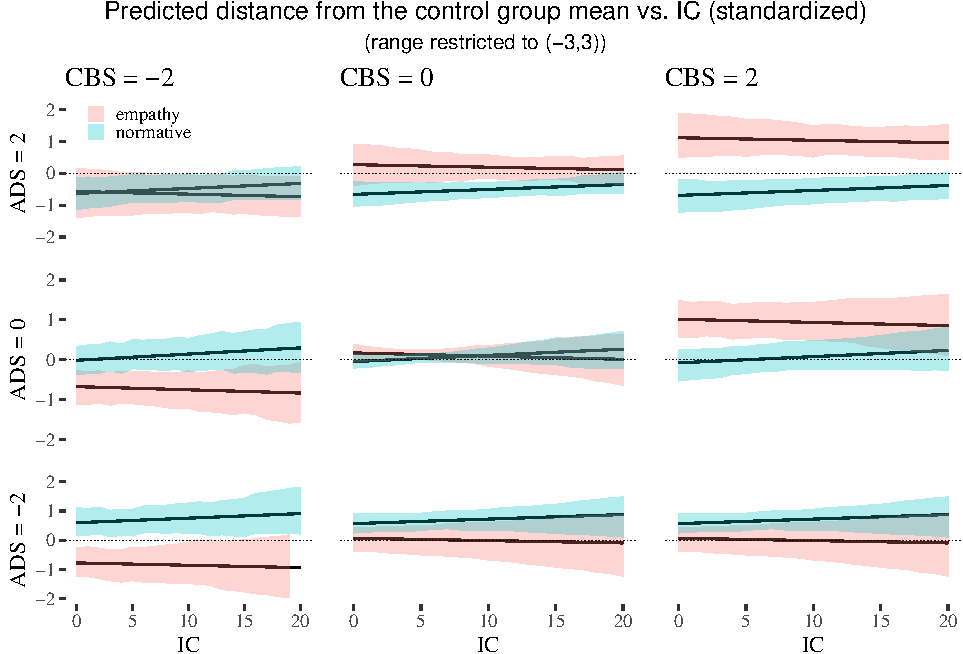
\includegraphics[width=1\linewidth]{bayesianReport3_files/figure-latex/unnamed-chunk-15-1} \end{center}

\normalsize

\section{Direct effect}\label{direct-effect}

Models for the evaluation of direct effect need to close the indirect
causal path from the treatment variables to the output, and they do so
by conditioning on \textsf{CAS}. Again, we face model selection. We
repeat all the model structures from the previous section, except for
now, each model is extended with \textsf{CAS} as a predictor. This time
the model structure we called \textsf{tooFar} turns out to do better. We
also consider extending it with interactions between \textsf{CAS} and
\textsf{IT} and \textsf{IC} (jointly and separately), but this results
in no further improvement.

\vspace{1mm} \footnotesize

\begin{Shaded}
\begin{Highlighting}[]
\NormalTok{nullDirect <-}\StringTok{ }\KeywordTok{quap}\NormalTok{(}
  \KeywordTok{alist}\NormalTok{(}
\NormalTok{    AdiffS }\OperatorTok{~}\StringTok{ }\KeywordTok{dnorm}\NormalTok{( mu, sigma ),}
\NormalTok{    mu <-}\StringTok{ }\NormalTok{a }\OperatorTok{+}\StringTok{ }\NormalTok{bCAS }\OperatorTok{*}\StringTok{ }\NormalTok{CAS,}
\NormalTok{    a }\OperatorTok{~}\StringTok{ }\KeywordTok{dnorm}\NormalTok{ (}\DecValTok{0}\NormalTok{,}\FloatTok{0.3}\NormalTok{),}
\NormalTok{    bCAS }\OperatorTok{~}\StringTok{ }\KeywordTok{dnorm}\NormalTok{(}\DecValTok{0}\NormalTok{,}\FloatTok{0.3}\NormalTok{),}
\NormalTok{    sigma  }\OperatorTok{~}\StringTok{ }\KeywordTok{dexp}\NormalTok{(}\DecValTok{1}\NormalTok{)}
\NormalTok{  ), }
  \DataTypeTok{data =}\NormalTok{ summaries  }
\NormalTok{)}

\NormalTok{ADSDirect <-}\StringTok{ }\KeywordTok{quap}\NormalTok{(}
  \KeywordTok{alist}\NormalTok{(}
\NormalTok{    AdiffS }\OperatorTok{~}\StringTok{ }\KeywordTok{dnorm}\NormalTok{( mu, sigma ),}
\NormalTok{    mu <-}\StringTok{  }\NormalTok{a }\OperatorTok{+}\StringTok{ }\NormalTok{bADS }\OperatorTok{*}\StringTok{ }\NormalTok{ADS}\OperatorTok{+}\StringTok{ }\NormalTok{bCAS }\OperatorTok{*}\StringTok{ }\NormalTok{CAS,}
\NormalTok{    a }\OperatorTok{~}\StringTok{ }\KeywordTok{dnorm}\NormalTok{ (}\DecValTok{0}\NormalTok{,}\FloatTok{0.3}\NormalTok{),}
\NormalTok{    bADS }\OperatorTok{~}\StringTok{ }\KeywordTok{dnorm}\NormalTok{(}\DecValTok{0}\NormalTok{,}\FloatTok{0.3}\NormalTok{),}
\NormalTok{    bCAS }\OperatorTok{~}\StringTok{ }\KeywordTok{dnorm}\NormalTok{(}\DecValTok{0}\NormalTok{,}\FloatTok{0.3}\NormalTok{),}
\NormalTok{    sigma  }\OperatorTok{~}\StringTok{ }\KeywordTok{dexp}\NormalTok{(}\DecValTok{1}\NormalTok{)}
\NormalTok{  ), }
  \DataTypeTok{data =}\NormalTok{ summaries}
\NormalTok{)}

\NormalTok{ADSICDirect <-}\StringTok{ }\KeywordTok{quap}\NormalTok{(}
  \KeywordTok{alist}\NormalTok{(}
\NormalTok{    AdiffS }\OperatorTok{~}\StringTok{ }\KeywordTok{dnorm}\NormalTok{( mu, sigma ),}
\NormalTok{    mu <-}\StringTok{  }\NormalTok{a }\OperatorTok{+}\StringTok{ }\NormalTok{bADS }\OperatorTok{*}\StringTok{ }\NormalTok{ADS}\OperatorTok{+}\StringTok{ }\NormalTok{bIC }\OperatorTok{*}\StringTok{ }\NormalTok{IC}\OperatorTok{+}\StringTok{ }\NormalTok{bCAS }\OperatorTok{*}\StringTok{ }\NormalTok{CAS,}
\NormalTok{    a }\OperatorTok{~}\StringTok{ }\KeywordTok{dnorm}\NormalTok{ (}\DecValTok{0}\NormalTok{,}\FloatTok{0.3}\NormalTok{),}
\NormalTok{    bADS }\OperatorTok{~}\StringTok{ }\KeywordTok{dnorm}\NormalTok{(}\DecValTok{0}\NormalTok{,}\FloatTok{0.3}\NormalTok{),}
\NormalTok{    bIC }\OperatorTok{~}\StringTok{ }\KeywordTok{dnorm}\NormalTok{(}\DecValTok{0}\NormalTok{,}\FloatTok{0.3}\NormalTok{),}
\NormalTok{    bCAS }\OperatorTok{~}\StringTok{ }\KeywordTok{dnorm}\NormalTok{(}\DecValTok{0}\NormalTok{,}\FloatTok{0.3}\NormalTok{),}
\NormalTok{    sigma  }\OperatorTok{~}\StringTok{ }\KeywordTok{dexp}\NormalTok{(}\DecValTok{1}\NormalTok{)}
\NormalTok{  ), }
  \DataTypeTok{data =}\NormalTok{ summaries}
\NormalTok{)}

\NormalTok{ITDirect <-}\StringTok{ }\KeywordTok{quap}\NormalTok{(}
  \KeywordTok{alist}\NormalTok{(}
\NormalTok{    AdiffS }\OperatorTok{~}\StringTok{ }\KeywordTok{dnorm}\NormalTok{( mu, sigma ),}
\NormalTok{    mu <-}\StringTok{  }\NormalTok{bIT[groupID] }\OperatorTok{+}\StringTok{ }\NormalTok{bCAS }\OperatorTok{*}\StringTok{ }\NormalTok{CAS,}
\NormalTok{    bIT[groupID] }\OperatorTok{~}\StringTok{ }\KeywordTok{dnorm}\NormalTok{(}\DecValTok{0}\NormalTok{,.}\DecValTok{3}\NormalTok{),}
\NormalTok{    bCAS }\OperatorTok{~}\StringTok{ }\KeywordTok{dnorm}\NormalTok{(}\DecValTok{0}\NormalTok{,}\FloatTok{0.3}\NormalTok{),}
\NormalTok{    sigma  }\OperatorTok{~}\StringTok{ }\KeywordTok{dexp}\NormalTok{(}\DecValTok{1}\NormalTok{)}
\NormalTok{  ), }
  \DataTypeTok{data =}\NormalTok{ summaries}
\NormalTok{)}

\NormalTok{ADSITDirect <-}\StringTok{ }\KeywordTok{quap}\NormalTok{(}
  \KeywordTok{alist}\NormalTok{(}
\NormalTok{    AdiffS }\OperatorTok{~}\StringTok{ }\KeywordTok{dnorm}\NormalTok{( mu, sigma ),}
\NormalTok{    mu <-}\StringTok{ }\NormalTok{a }\OperatorTok{+}\StringTok{ }\NormalTok{bADS }\OperatorTok{*}\StringTok{ }\NormalTok{ADS }\OperatorTok{+}\StringTok{  }\NormalTok{bIT[groupID]}\OperatorTok{+}\StringTok{ }\NormalTok{bCAS }\OperatorTok{*}\StringTok{ }\NormalTok{CAS,}
\NormalTok{    a }\OperatorTok{~}\StringTok{ }\KeywordTok{dnorm}\NormalTok{ (}\DecValTok{0}\NormalTok{,}\FloatTok{0.3}\NormalTok{),}
\NormalTok{    bADS }\OperatorTok{~}\StringTok{ }\KeywordTok{dnorm}\NormalTok{(}\DecValTok{0}\NormalTok{,.}\DecValTok{3}\NormalTok{),}
\NormalTok{    bCAS }\OperatorTok{~}\StringTok{ }\KeywordTok{dnorm}\NormalTok{(}\DecValTok{0}\NormalTok{,}\FloatTok{0.3}\NormalTok{),}
\NormalTok{    bIT[groupID] }\OperatorTok{~}\StringTok{ }\KeywordTok{dnorm}\NormalTok{(}\DecValTok{0}\NormalTok{,.}\DecValTok{3}\NormalTok{),}
\NormalTok{    sigma  }\OperatorTok{~}\StringTok{ }\KeywordTok{dexp}\NormalTok{(}\DecValTok{1}\NormalTok{)}
\NormalTok{  ), }
  \DataTypeTok{data =}\NormalTok{ summaries}
\NormalTok{)}


\NormalTok{ADSITICDirect <-}\StringTok{ }\KeywordTok{quap}\NormalTok{(}
  \KeywordTok{alist}\NormalTok{(}
\NormalTok{    AdiffS }\OperatorTok{~}\StringTok{ }\KeywordTok{dnorm}\NormalTok{( mu, sigma ),}
\NormalTok{    mu <-}\StringTok{ }\NormalTok{a }\OperatorTok{+}\StringTok{ }\NormalTok{bADS }\OperatorTok{*}\StringTok{ }\NormalTok{ADS }\OperatorTok{+}\StringTok{  }\NormalTok{bIT[groupID] }\OperatorTok{+}\StringTok{ }\NormalTok{bIC }\OperatorTok{*}\StringTok{ }\NormalTok{IC}\OperatorTok{+}\StringTok{ }\NormalTok{bCAS }\OperatorTok{*}\StringTok{ }\NormalTok{CAS,}
\NormalTok{    a }\OperatorTok{~}\StringTok{ }\KeywordTok{dnorm}\NormalTok{ (}\DecValTok{0}\NormalTok{,}\FloatTok{0.3}\NormalTok{),}
\NormalTok{    bADS }\OperatorTok{~}\StringTok{ }\KeywordTok{dnorm}\NormalTok{(}\DecValTok{0}\NormalTok{,.}\DecValTok{3}\NormalTok{),}
\NormalTok{    bCAS }\OperatorTok{~}\StringTok{ }\KeywordTok{dnorm}\NormalTok{(}\DecValTok{0}\NormalTok{,}\FloatTok{0.3}\NormalTok{),}
\NormalTok{    bIT[groupID] }\OperatorTok{~}\StringTok{ }\KeywordTok{dnorm}\NormalTok{(}\DecValTok{0}\NormalTok{,.}\DecValTok{3}\NormalTok{),}
\NormalTok{    bIC }\OperatorTok{~}\StringTok{ }\KeywordTok{dnorm}\NormalTok{(}\DecValTok{0}\NormalTok{,.}\DecValTok{3}\NormalTok{),}
\NormalTok{    sigma  }\OperatorTok{~}\StringTok{ }\KeywordTok{dexp}\NormalTok{(}\DecValTok{1}\NormalTok{)}
\NormalTok{  ), }
  \DataTypeTok{data =}\NormalTok{ summaries}
\NormalTok{)}


\NormalTok{ADSITIC_ADSICDirect <-}\StringTok{ }\KeywordTok{quap}\NormalTok{(}
  \KeywordTok{alist}\NormalTok{(}
\NormalTok{    AdiffS }\OperatorTok{~}\StringTok{ }\KeywordTok{dnorm}\NormalTok{( mu, sigma ),}
\NormalTok{    mu <-}\StringTok{ }\NormalTok{a }\OperatorTok{+}\StringTok{ }\NormalTok{bADS }\OperatorTok{*}\StringTok{ }\NormalTok{ADS }\OperatorTok{+}\StringTok{  }\NormalTok{bIT[groupID] }\OperatorTok{+}\StringTok{ }\NormalTok{bIC }\OperatorTok{*}\StringTok{ }\NormalTok{IC }\OperatorTok{+}\StringTok{ }\NormalTok{bADSIC }\OperatorTok{*}\StringTok{ }\NormalTok{ADS }\OperatorTok{*}\StringTok{ }\NormalTok{IC}\OperatorTok{+}\StringTok{ }\NormalTok{bCAS }\OperatorTok{*}\StringTok{ }\NormalTok{CAS,}
\NormalTok{    a }\OperatorTok{~}\StringTok{ }\KeywordTok{dnorm}\NormalTok{ (}\DecValTok{0}\NormalTok{,}\FloatTok{0.3}\NormalTok{),}
\NormalTok{    bADS }\OperatorTok{~}\StringTok{ }\KeywordTok{dnorm}\NormalTok{(}\DecValTok{0}\NormalTok{,.}\DecValTok{3}\NormalTok{),}
\NormalTok{    bCAS }\OperatorTok{~}\StringTok{ }\KeywordTok{dnorm}\NormalTok{(}\DecValTok{0}\NormalTok{,}\FloatTok{0.3}\NormalTok{),}
\NormalTok{    bADSIC }\OperatorTok{~}\StringTok{ }\KeywordTok{dnorm}\NormalTok{(}\DecValTok{0}\NormalTok{,.}\DecValTok{3}\NormalTok{),}
\NormalTok{    bIT[groupID] }\OperatorTok{~}\StringTok{ }\KeywordTok{dnorm}\NormalTok{(}\DecValTok{0}\NormalTok{,.}\DecValTok{3}\NormalTok{),}
\NormalTok{    bIC }\OperatorTok{~}\StringTok{ }\KeywordTok{dnorm}\NormalTok{(}\DecValTok{0}\NormalTok{,.}\DecValTok{3}\NormalTok{),}
\NormalTok{    sigma  }\OperatorTok{~}\StringTok{ }\KeywordTok{dexp}\NormalTok{(}\DecValTok{1}\NormalTok{)}
\NormalTok{  ), }
  \DataTypeTok{data =}\NormalTok{ summaries}
\NormalTok{)}


\NormalTok{ADSITIC_ADSIC_ADSITDirect <-}\StringTok{ }\KeywordTok{quap}\NormalTok{(}
  \KeywordTok{alist}\NormalTok{(}
\NormalTok{    AdiffS }\OperatorTok{~}\StringTok{ }\KeywordTok{dnorm}\NormalTok{( mu, sigma ),}
\NormalTok{    mu <-}\StringTok{ }\NormalTok{a }\OperatorTok{+}\StringTok{ }\NormalTok{bADS[groupID] }\OperatorTok{*}\StringTok{ }\NormalTok{ADS }\OperatorTok{+}\StringTok{  }\NormalTok{bIT[groupID] }\OperatorTok{+}\StringTok{ }\NormalTok{bIC }\OperatorTok{*}\StringTok{ }\NormalTok{IC }\OperatorTok{+}\StringTok{ }\NormalTok{bADSIC }\OperatorTok{*}\StringTok{ }\NormalTok{ADS }\OperatorTok{*}\StringTok{ }\NormalTok{IC}\OperatorTok{+}\StringTok{ }\NormalTok{bCAS }\OperatorTok{*}\StringTok{ }\NormalTok{CAS,}
\NormalTok{    a }\OperatorTok{~}\StringTok{ }\KeywordTok{dnorm}\NormalTok{ (}\DecValTok{0}\NormalTok{,}\FloatTok{0.3}\NormalTok{),}
\NormalTok{    bADS[groupID] }\OperatorTok{~}\StringTok{ }\KeywordTok{dnorm}\NormalTok{(}\DecValTok{0}\NormalTok{,.}\DecValTok{3}\NormalTok{),}
\NormalTok{    bADSIC }\OperatorTok{~}\StringTok{ }\KeywordTok{dnorm}\NormalTok{(}\DecValTok{0}\NormalTok{,.}\DecValTok{3}\NormalTok{),}
\NormalTok{    bCAS }\OperatorTok{~}\StringTok{ }\KeywordTok{dnorm}\NormalTok{(}\DecValTok{0}\NormalTok{,}\FloatTok{0.3}\NormalTok{),}
\NormalTok{    bIT[groupID] }\OperatorTok{~}\StringTok{ }\KeywordTok{dnorm}\NormalTok{(}\DecValTok{0}\NormalTok{,.}\DecValTok{3}\NormalTok{),}
\NormalTok{    bIC }\OperatorTok{~}\StringTok{ }\KeywordTok{dnorm}\NormalTok{(}\DecValTok{0}\NormalTok{,.}\DecValTok{3}\NormalTok{),}
\NormalTok{    sigma  }\OperatorTok{~}\StringTok{ }\KeywordTok{dexp}\NormalTok{(}\DecValTok{1}\NormalTok{)}
\NormalTok{  ), }
  \DataTypeTok{data =}\NormalTok{ summaries}
\NormalTok{)}


\NormalTok{ADSIT_ADSITDirect <-}\StringTok{ }\KeywordTok{quap}\NormalTok{(}
  \KeywordTok{alist}\NormalTok{(}
\NormalTok{    AdiffS }\OperatorTok{~}\StringTok{ }\KeywordTok{dnorm}\NormalTok{( mu, sigma ),}
\NormalTok{    mu <-}\StringTok{ }\NormalTok{a }\OperatorTok{+}\StringTok{ }\NormalTok{bADS[groupID] }\OperatorTok{*}\StringTok{ }\NormalTok{ADS }\OperatorTok{+}\StringTok{  }\NormalTok{bIT[groupID] }\OperatorTok{+}\StringTok{ }\NormalTok{bCAS }\OperatorTok{*}\StringTok{ }\NormalTok{CAS,}
\NormalTok{    a }\OperatorTok{~}\StringTok{ }\KeywordTok{dnorm}\NormalTok{ (}\DecValTok{0}\NormalTok{,}\FloatTok{0.3}\NormalTok{),}
\NormalTok{    bADS[groupID] }\OperatorTok{~}\StringTok{ }\KeywordTok{dnorm}\NormalTok{(}\DecValTok{0}\NormalTok{,.}\DecValTok{3}\NormalTok{),}
    \CommentTok{#bADSIC ~ dnorm(0,.5),}
\NormalTok{    bIT[groupID] }\OperatorTok{~}\StringTok{ }\KeywordTok{dnorm}\NormalTok{(}\DecValTok{0}\NormalTok{,.}\DecValTok{3}\NormalTok{),}
    \CommentTok{#bIC ~ dnorm(0,.5),}
\NormalTok{    bCAS }\OperatorTok{~}\StringTok{ }\KeywordTok{dnorm}\NormalTok{(}\DecValTok{0}\NormalTok{,}\FloatTok{0.3}\NormalTok{),}
\NormalTok{    sigma  }\OperatorTok{~}\StringTok{ }\KeywordTok{dexp}\NormalTok{(}\DecValTok{1}\NormalTok{)}
\NormalTok{  ), }
  \DataTypeTok{data =}\NormalTok{ summaries}
\NormalTok{)}


\NormalTok{ADSITIC_ADSIT_ITIC_ADSICDirect <-}\StringTok{ }\KeywordTok{quap}\NormalTok{(}
  \KeywordTok{alist}\NormalTok{(}
\NormalTok{    AdiffS }\OperatorTok{~}\StringTok{ }\KeywordTok{dnorm}\NormalTok{( mu, sigma ),}
\NormalTok{    mu <-}\StringTok{ }\NormalTok{a }\OperatorTok{+}\StringTok{ }\NormalTok{bADS[groupID] }\OperatorTok{*}\StringTok{ }\NormalTok{ADS }\OperatorTok{+}\StringTok{  }\NormalTok{bIT[groupID] }\OperatorTok{+}\StringTok{ }\NormalTok{bIC[groupID] }\OperatorTok{*}\StringTok{ }\NormalTok{IC }\OperatorTok{+}
\StringTok{      }\NormalTok{bADSIC }\OperatorTok{*}\StringTok{ }\NormalTok{ADS }\OperatorTok{*}\StringTok{ }\NormalTok{IC }\OperatorTok{+}\StringTok{ }\NormalTok{bCAS }\OperatorTok{*}\StringTok{ }\NormalTok{CAS,}
\NormalTok{    a }\OperatorTok{~}\StringTok{ }\KeywordTok{dnorm}\NormalTok{ (}\DecValTok{0}\NormalTok{,}\FloatTok{0.3}\NormalTok{),}
\NormalTok{    bADS[groupID] }\OperatorTok{~}\StringTok{ }\KeywordTok{dnorm}\NormalTok{(}\DecValTok{0}\NormalTok{,.}\DecValTok{3}\NormalTok{),}
\NormalTok{    bADSIC }\OperatorTok{~}\StringTok{ }\KeywordTok{dnorm}\NormalTok{(}\DecValTok{0}\NormalTok{,.}\DecValTok{3}\NormalTok{),}
\NormalTok{    bCAS }\OperatorTok{~}\StringTok{ }\KeywordTok{dnorm}\NormalTok{(}\DecValTok{0}\NormalTok{,}\FloatTok{0.3}\NormalTok{),}
\NormalTok{    bIT[groupID] }\OperatorTok{~}\StringTok{ }\KeywordTok{dnorm}\NormalTok{(}\DecValTok{0}\NormalTok{,.}\DecValTok{3}\NormalTok{),}
\NormalTok{    bIC[groupID] }\OperatorTok{~}\StringTok{ }\KeywordTok{dnorm}\NormalTok{(}\DecValTok{0}\NormalTok{,.}\DecValTok{3}\NormalTok{),}
\NormalTok{    sigma  }\OperatorTok{~}\StringTok{ }\KeywordTok{dexp}\NormalTok{(}\DecValTok{1}\NormalTok{)}
\NormalTok{  ), }
  \DataTypeTok{data =}\NormalTok{ summaries}
\NormalTok{)}


\NormalTok{ADSITICCBS_ITIC_ADSICDirect <-}\StringTok{ }\KeywordTok{quap}\NormalTok{(}
  \KeywordTok{alist}\NormalTok{(}
\NormalTok{    AdiffS }\OperatorTok{~}\StringTok{ }\KeywordTok{dnorm}\NormalTok{( mu, sigma ),}
\NormalTok{    mu <-}\StringTok{ }\NormalTok{a }\OperatorTok{+}\StringTok{ }\NormalTok{bADS[groupID] }\OperatorTok{*}\StringTok{ }\NormalTok{ADS }\OperatorTok{+}\StringTok{  }\NormalTok{bIT[groupID] }\OperatorTok{+}\StringTok{ }\NormalTok{bIC[groupID] }\OperatorTok{*}\StringTok{ }\NormalTok{IC }\OperatorTok{+}\StringTok{ }
\StringTok{      }\NormalTok{bADSIC }\OperatorTok{*}\StringTok{ }\NormalTok{ADS }\OperatorTok{*}\StringTok{ }\NormalTok{IC}\OperatorTok{+}\StringTok{ }\NormalTok{bCBS }\OperatorTok{*}\NormalTok{CBS }\OperatorTok{+}\StringTok{ }\NormalTok{bCAS }\OperatorTok{*}\StringTok{ }\NormalTok{CAS,}
\NormalTok{    a }\OperatorTok{~}\StringTok{ }\KeywordTok{dnorm}\NormalTok{ (}\DecValTok{0}\NormalTok{,}\FloatTok{0.3}\NormalTok{),}
\NormalTok{    bADS[groupID] }\OperatorTok{~}\StringTok{ }\KeywordTok{dnorm}\NormalTok{(}\DecValTok{0}\NormalTok{,.}\DecValTok{3}\NormalTok{),}
\NormalTok{    bADSIC }\OperatorTok{~}\StringTok{ }\KeywordTok{dnorm}\NormalTok{(}\DecValTok{0}\NormalTok{,.}\DecValTok{3}\NormalTok{),}
\NormalTok{    bCBS }\OperatorTok{~}\StringTok{ }\KeywordTok{dnorm}\NormalTok{(}\DecValTok{0}\NormalTok{,.}\DecValTok{3}\NormalTok{),}
\NormalTok{    bCAS }\OperatorTok{~}\StringTok{ }\KeywordTok{dnorm}\NormalTok{(}\DecValTok{0}\NormalTok{,}\FloatTok{0.3}\NormalTok{),}
\NormalTok{    bIT[groupID] }\OperatorTok{~}\StringTok{ }\KeywordTok{dnorm}\NormalTok{(}\DecValTok{0}\NormalTok{,.}\DecValTok{3}\NormalTok{),}
\NormalTok{    bIC[groupID] }\OperatorTok{~}\StringTok{ }\KeywordTok{dnorm}\NormalTok{(}\DecValTok{0}\NormalTok{,.}\DecValTok{3}\NormalTok{),}
\NormalTok{    sigma  }\OperatorTok{~}\StringTok{ }\KeywordTok{dexp}\NormalTok{(}\DecValTok{1}\NormalTok{)}
\NormalTok{  ), }
  \DataTypeTok{data =}\NormalTok{ summaries}
\NormalTok{)}


\NormalTok{FinalDirect <-}\StringTok{ }\KeywordTok{quap}\NormalTok{(}
  \KeywordTok{alist}\NormalTok{(}
\NormalTok{    AdiffS }\OperatorTok{~}\StringTok{ }\KeywordTok{dnorm}\NormalTok{( mu, sigma ),}
\NormalTok{    mu <-}\StringTok{ }\NormalTok{a }\OperatorTok{+}\StringTok{ }\NormalTok{bADS[groupID] }\OperatorTok{*}\StringTok{ }\NormalTok{ADS }\OperatorTok{+}\StringTok{  }\NormalTok{bIT[groupID] }\OperatorTok{+}\StringTok{ }\NormalTok{bIC[groupID] }\OperatorTok{*}\StringTok{ }\NormalTok{IC }\OperatorTok{+}\StringTok{ }
\StringTok{      }\NormalTok{bADSIC }\OperatorTok{*}\StringTok{ }\NormalTok{ADS }\OperatorTok{*}\StringTok{ }\NormalTok{IC}\OperatorTok{+}\StringTok{ }\NormalTok{bCBS[groupID] }\OperatorTok{*}\NormalTok{CBS }\OperatorTok{+}\StringTok{ }\NormalTok{bCAS }\OperatorTok{*}\StringTok{ }\NormalTok{CAS,}
\NormalTok{    a }\OperatorTok{~}\StringTok{ }\KeywordTok{dnorm}\NormalTok{ (}\DecValTok{0}\NormalTok{,}\FloatTok{0.3}\NormalTok{),}
\NormalTok{    bADS[groupID] }\OperatorTok{~}\StringTok{ }\KeywordTok{dnorm}\NormalTok{(}\DecValTok{0}\NormalTok{,.}\DecValTok{3}\NormalTok{),}
\NormalTok{    bADSIC }\OperatorTok{~}\StringTok{ }\KeywordTok{dnorm}\NormalTok{(}\DecValTok{0}\NormalTok{,.}\DecValTok{3}\NormalTok{),}
\NormalTok{    bCAS }\OperatorTok{~}\StringTok{ }\KeywordTok{dnorm}\NormalTok{(}\DecValTok{0}\NormalTok{,}\FloatTok{0.3}\NormalTok{),}
\NormalTok{    bCBS[groupID] }\OperatorTok{~}\StringTok{ }\KeywordTok{dnorm}\NormalTok{(}\DecValTok{0}\NormalTok{,.}\DecValTok{3}\NormalTok{),}
\NormalTok{    bIT[groupID] }\OperatorTok{~}\StringTok{ }\KeywordTok{dnorm}\NormalTok{(}\DecValTok{0}\NormalTok{,.}\DecValTok{3}\NormalTok{),}
\NormalTok{    bIC[groupID] }\OperatorTok{~}\StringTok{ }\KeywordTok{dnorm}\NormalTok{(}\DecValTok{0}\NormalTok{,.}\DecValTok{3}\NormalTok{),}
\NormalTok{    sigma  }\OperatorTok{~}\StringTok{ }\KeywordTok{dexp}\NormalTok{(}\DecValTok{1}\NormalTok{)}
\NormalTok{  ), }
  \DataTypeTok{data =}\NormalTok{ summaries}
\NormalTok{)}



\NormalTok{tooFarDirect <-}\StringTok{ }\KeywordTok{quap}\NormalTok{(}
  \KeywordTok{alist}\NormalTok{(}
\NormalTok{    AdiffS }\OperatorTok{~}\StringTok{ }\KeywordTok{dnorm}\NormalTok{( mu, sigma ),}
\NormalTok{    mu <-}\StringTok{ }\NormalTok{a }\OperatorTok{+}\StringTok{ }\NormalTok{bADS[groupID] }\OperatorTok{*}\StringTok{ }\NormalTok{ADS }\OperatorTok{+}\StringTok{  }\NormalTok{bIT[groupID] }\OperatorTok{+}\StringTok{ }\NormalTok{bIC[groupID] }\OperatorTok{*}\StringTok{ }\NormalTok{IC }\OperatorTok{+}\StringTok{ }
\StringTok{      }\NormalTok{bADSIC }\OperatorTok{*}\StringTok{ }\NormalTok{ADS }\OperatorTok{*}\StringTok{ }\NormalTok{IC}\OperatorTok{+}\StringTok{ }\NormalTok{bCBS[groupID] }\OperatorTok{*}\NormalTok{CBS }\OperatorTok{+}\StringTok{ }\NormalTok{bCBSIC }\OperatorTok{*}\StringTok{ }\NormalTok{CBS }\OperatorTok{*}\StringTok{ }\NormalTok{IC }\OperatorTok{+}\StringTok{ }\NormalTok{bCAS }\OperatorTok{*}\StringTok{ }\NormalTok{CAS, }
\NormalTok{    a }\OperatorTok{~}\StringTok{ }\KeywordTok{dnorm}\NormalTok{ (}\DecValTok{0}\NormalTok{,}\FloatTok{0.3}\NormalTok{),}
\NormalTok{    bADS[groupID] }\OperatorTok{~}\StringTok{ }\KeywordTok{dnorm}\NormalTok{(}\DecValTok{0}\NormalTok{,.}\DecValTok{3}\NormalTok{),}
\NormalTok{    bADSIC }\OperatorTok{~}\StringTok{ }\KeywordTok{dnorm}\NormalTok{(}\DecValTok{0}\NormalTok{,.}\DecValTok{3}\NormalTok{),}
\NormalTok{    bCAS }\OperatorTok{~}\StringTok{ }\KeywordTok{dnorm}\NormalTok{(}\DecValTok{0}\NormalTok{,}\FloatTok{0.3}\NormalTok{),}
\NormalTok{    bCBS[groupID] }\OperatorTok{~}\StringTok{ }\KeywordTok{dnorm}\NormalTok{(}\DecValTok{0}\NormalTok{,.}\DecValTok{3}\NormalTok{),}
\NormalTok{    bIT[groupID] }\OperatorTok{~}\StringTok{ }\KeywordTok{dnorm}\NormalTok{(}\DecValTok{0}\NormalTok{,.}\DecValTok{3}\NormalTok{),}
\NormalTok{    bIC[groupID] }\OperatorTok{~}\StringTok{ }\KeywordTok{dnorm}\NormalTok{(}\DecValTok{0}\NormalTok{,.}\DecValTok{3}\NormalTok{),}
\NormalTok{    bCBSIC }\OperatorTok{~}\StringTok{ }\KeywordTok{dnorm}\NormalTok{(}\DecValTok{0}\NormalTok{, }\FloatTok{.3}\NormalTok{),}
\NormalTok{    sigma  }\OperatorTok{~}\StringTok{ }\KeywordTok{dexp}\NormalTok{(}\DecValTok{1}\NormalTok{)}
\NormalTok{  ), }
  \DataTypeTok{data =}\NormalTok{ summaries}
\NormalTok{)}




\NormalTok{tooFarDirect_CASIT <-}\StringTok{ }\KeywordTok{quap}\NormalTok{(}
  \KeywordTok{alist}\NormalTok{(}
\NormalTok{    AdiffS }\OperatorTok{~}\StringTok{ }\KeywordTok{dnorm}\NormalTok{( mu, sigma ),}
\NormalTok{    mu <-}\StringTok{ }\NormalTok{a }\OperatorTok{+}\StringTok{ }\NormalTok{bADS[groupID] }\OperatorTok{*}\StringTok{ }\NormalTok{ADS }\OperatorTok{+}\StringTok{  }\NormalTok{bIT[groupID] }\OperatorTok{+}\StringTok{ }\NormalTok{bIC[groupID] }\OperatorTok{*}\StringTok{ }\NormalTok{IC }\OperatorTok{+}\StringTok{ }
\StringTok{      }\NormalTok{bADSIC }\OperatorTok{*}\StringTok{ }\NormalTok{ADS }\OperatorTok{*}\StringTok{ }\NormalTok{IC}\OperatorTok{+}\StringTok{ }\NormalTok{bCBS[groupID] }\OperatorTok{*}\NormalTok{CBS }\OperatorTok{+}\StringTok{ }\NormalTok{bCBSIC }\OperatorTok{*}\StringTok{ }\NormalTok{CBS }\OperatorTok{*}\StringTok{ }\NormalTok{IC }\OperatorTok{+}\StringTok{ }\NormalTok{bCAS[groupID] }\OperatorTok{*}\StringTok{ }\NormalTok{CAS, }
\NormalTok{    a }\OperatorTok{~}\StringTok{ }\KeywordTok{dnorm}\NormalTok{ (}\DecValTok{0}\NormalTok{,}\FloatTok{0.3}\NormalTok{),}
\NormalTok{    bADS[groupID] }\OperatorTok{~}\StringTok{ }\KeywordTok{dnorm}\NormalTok{(}\DecValTok{0}\NormalTok{,.}\DecValTok{3}\NormalTok{),}
\NormalTok{    bADSIC }\OperatorTok{~}\StringTok{ }\KeywordTok{dnorm}\NormalTok{(}\DecValTok{0}\NormalTok{,.}\DecValTok{3}\NormalTok{),}
\NormalTok{    bCAS[groupID] }\OperatorTok{~}\StringTok{ }\KeywordTok{dnorm}\NormalTok{(}\DecValTok{0}\NormalTok{,}\FloatTok{0.3}\NormalTok{),}
\NormalTok{    bCBS[groupID] }\OperatorTok{~}\StringTok{ }\KeywordTok{dnorm}\NormalTok{(}\DecValTok{0}\NormalTok{,.}\DecValTok{3}\NormalTok{),}
\NormalTok{    bIT[groupID] }\OperatorTok{~}\StringTok{ }\KeywordTok{dnorm}\NormalTok{(}\DecValTok{0}\NormalTok{,.}\DecValTok{3}\NormalTok{),}
\NormalTok{    bIC[groupID] }\OperatorTok{~}\StringTok{ }\KeywordTok{dnorm}\NormalTok{(}\DecValTok{0}\NormalTok{,.}\DecValTok{3}\NormalTok{),}
\NormalTok{    bCBSIC }\OperatorTok{~}\StringTok{ }\KeywordTok{dnorm}\NormalTok{(}\DecValTok{0}\NormalTok{, }\FloatTok{.3}\NormalTok{),}
\NormalTok{    sigma  }\OperatorTok{~}\StringTok{ }\KeywordTok{dexp}\NormalTok{(}\DecValTok{1}\NormalTok{)}
\NormalTok{  ), }
  \DataTypeTok{data =}\NormalTok{ summaries}
\NormalTok{)}



\NormalTok{tooFarDirect_CASIC <-}\StringTok{ }\KeywordTok{quap}\NormalTok{(}
  \KeywordTok{alist}\NormalTok{(}
\NormalTok{    AdiffS }\OperatorTok{~}\StringTok{ }\KeywordTok{dnorm}\NormalTok{( mu, sigma ),}
\NormalTok{    mu <-}\StringTok{ }\NormalTok{a }\OperatorTok{+}\StringTok{ }\NormalTok{bADS[groupID] }\OperatorTok{*}\StringTok{ }\NormalTok{ADS }\OperatorTok{+}\StringTok{  }\NormalTok{bIT[groupID] }\OperatorTok{+}\StringTok{ }\NormalTok{bIC[groupID] }\OperatorTok{*}\StringTok{ }\NormalTok{IC }\OperatorTok{+}\StringTok{ }
\StringTok{      }\NormalTok{bADSIC }\OperatorTok{*}\StringTok{ }\NormalTok{ADS }\OperatorTok{*}\StringTok{ }\NormalTok{IC}\OperatorTok{+}\StringTok{ }\NormalTok{bCBS[groupID] }\OperatorTok{*}\NormalTok{CBS }\OperatorTok{+}\StringTok{ }\NormalTok{bCBSIC }\OperatorTok{*}\StringTok{ }\NormalTok{CBS }\OperatorTok{*}\StringTok{ }\NormalTok{IC }\OperatorTok{+}\StringTok{ }\NormalTok{bCAS }\OperatorTok{*}\StringTok{ }\NormalTok{CAS }\OperatorTok{+}\StringTok{ }\NormalTok{bCASIC }\OperatorTok{*}\StringTok{ }\NormalTok{CAS }\OperatorTok{*}\StringTok{ }\NormalTok{IC, }
\NormalTok{    a }\OperatorTok{~}\StringTok{ }\KeywordTok{dnorm}\NormalTok{ (}\DecValTok{0}\NormalTok{,}\FloatTok{0.3}\NormalTok{),}
\NormalTok{    bADS[groupID] }\OperatorTok{~}\StringTok{ }\KeywordTok{dnorm}\NormalTok{(}\DecValTok{0}\NormalTok{,.}\DecValTok{3}\NormalTok{),}
\NormalTok{    bADSIC }\OperatorTok{~}\StringTok{ }\KeywordTok{dnorm}\NormalTok{(}\DecValTok{0}\NormalTok{,.}\DecValTok{3}\NormalTok{),}
\NormalTok{    bCAS }\OperatorTok{~}\StringTok{ }\KeywordTok{dnorm}\NormalTok{(}\DecValTok{0}\NormalTok{,}\FloatTok{0.3}\NormalTok{),}
\NormalTok{    bCASIC }\OperatorTok{~}\StringTok{ }\KeywordTok{dnorm}\NormalTok{(}\DecValTok{0}\NormalTok{,}\FloatTok{0.3}\NormalTok{),}
\NormalTok{    bCBS[groupID] }\OperatorTok{~}\StringTok{ }\KeywordTok{dnorm}\NormalTok{(}\DecValTok{0}\NormalTok{,.}\DecValTok{3}\NormalTok{),}
\NormalTok{    bIT[groupID] }\OperatorTok{~}\StringTok{ }\KeywordTok{dnorm}\NormalTok{(}\DecValTok{0}\NormalTok{,.}\DecValTok{3}\NormalTok{),}
\NormalTok{    bIC[groupID] }\OperatorTok{~}\StringTok{ }\KeywordTok{dnorm}\NormalTok{(}\DecValTok{0}\NormalTok{,.}\DecValTok{3}\NormalTok{),}
\NormalTok{    bCBSIC }\OperatorTok{~}\StringTok{ }\KeywordTok{dnorm}\NormalTok{(}\DecValTok{0}\NormalTok{, }\FloatTok{.3}\NormalTok{),}
\NormalTok{    sigma  }\OperatorTok{~}\StringTok{ }\KeywordTok{dexp}\NormalTok{(}\DecValTok{1}\NormalTok{)}
\NormalTok{  ), }
  \DataTypeTok{data =}\NormalTok{ summaries}
\NormalTok{)}


\NormalTok{tooFarDirect_CASIC_CASIT <-}\StringTok{ }\KeywordTok{quap}\NormalTok{(}
  \KeywordTok{alist}\NormalTok{(}
\NormalTok{    AdiffS }\OperatorTok{~}\StringTok{ }\KeywordTok{dnorm}\NormalTok{( mu, sigma ),}
\NormalTok{    mu <-}\StringTok{ }\NormalTok{a }\OperatorTok{+}\StringTok{ }\NormalTok{bADS[groupID] }\OperatorTok{*}\StringTok{ }\NormalTok{ADS }\OperatorTok{+}\StringTok{  }\NormalTok{bIT[groupID] }\OperatorTok{+}\StringTok{ }\NormalTok{bIC[groupID] }\OperatorTok{*}\StringTok{ }\NormalTok{IC }\OperatorTok{+}\StringTok{ }
\StringTok{      }\NormalTok{bADSIC }\OperatorTok{*}\StringTok{ }\NormalTok{ADS }\OperatorTok{*}\StringTok{ }\NormalTok{IC}\OperatorTok{+}\StringTok{ }\NormalTok{bCBS[groupID] }\OperatorTok{*}\NormalTok{CBS }\OperatorTok{+}\StringTok{ }\NormalTok{bCBSIC }\OperatorTok{*}\StringTok{ }\NormalTok{CBS }\OperatorTok{*}\StringTok{ }\NormalTok{IC }\OperatorTok{+}\StringTok{ }\NormalTok{bCAS[groupID] }\OperatorTok{*}\StringTok{ }\NormalTok{CAS }\OperatorTok{+}\StringTok{ }\NormalTok{bCASIC }\OperatorTok{*}\StringTok{ }\NormalTok{CAS }\OperatorTok{*}\StringTok{ }\NormalTok{IC, }
\NormalTok{    a }\OperatorTok{~}\StringTok{ }\KeywordTok{dnorm}\NormalTok{ (}\DecValTok{0}\NormalTok{,}\FloatTok{0.3}\NormalTok{),}
\NormalTok{    bADS[groupID] }\OperatorTok{~}\StringTok{ }\KeywordTok{dnorm}\NormalTok{(}\DecValTok{0}\NormalTok{,.}\DecValTok{3}\NormalTok{),}
\NormalTok{    bADSIC }\OperatorTok{~}\StringTok{ }\KeywordTok{dnorm}\NormalTok{(}\DecValTok{0}\NormalTok{,.}\DecValTok{3}\NormalTok{),}
\NormalTok{    bCAS[groupID] }\OperatorTok{~}\StringTok{ }\KeywordTok{dnorm}\NormalTok{(}\DecValTok{0}\NormalTok{,}\FloatTok{0.3}\NormalTok{),}
\NormalTok{    bCASIC }\OperatorTok{~}\StringTok{ }\KeywordTok{dnorm}\NormalTok{(}\DecValTok{0}\NormalTok{,}\FloatTok{0.3}\NormalTok{),}
\NormalTok{    bCBS[groupID] }\OperatorTok{~}\StringTok{ }\KeywordTok{dnorm}\NormalTok{(}\DecValTok{0}\NormalTok{,.}\DecValTok{3}\NormalTok{),}
\NormalTok{    bIT[groupID] }\OperatorTok{~}\StringTok{ }\KeywordTok{dnorm}\NormalTok{(}\DecValTok{0}\NormalTok{,.}\DecValTok{3}\NormalTok{),}
\NormalTok{    bIC[groupID] }\OperatorTok{~}\StringTok{ }\KeywordTok{dnorm}\NormalTok{(}\DecValTok{0}\NormalTok{,.}\DecValTok{3}\NormalTok{),}
\NormalTok{    bCBSIC }\OperatorTok{~}\StringTok{ }\KeywordTok{dnorm}\NormalTok{(}\DecValTok{0}\NormalTok{, }\FloatTok{.3}\NormalTok{),}
\NormalTok{    sigma  }\OperatorTok{~}\StringTok{ }\KeywordTok{dexp}\NormalTok{(}\DecValTok{1}\NormalTok{)}
\NormalTok{  ), }
  \DataTypeTok{data =}\NormalTok{ summaries}
\NormalTok{)}








\NormalTok{comparisonDirect<-}\StringTok{ }\KeywordTok{compare}\NormalTok{(nullDirect,ADSDirect,ADSICDirect,ITDirect,ADSITDirect,ADSITICDirect,ADSITIC_ADSICDirect, ADSITIC_ADSIC_ADSITDirect,ADSIT_ADSITDirect,ADSITIC_ADSIT_ITIC_ADSICDirect,}
\NormalTok{                     ADSITICCBS_ITIC_ADSICDirect,FinalDirect, tooFarDirect,tooFarDirect_CASIT,}
\NormalTok{                     tooFarDirect_CASIC,tooFarDirect_CASIC_CASIT)}


\KeywordTok{mykable}\NormalTok{(}\KeywordTok{round}\NormalTok{(}\KeywordTok{data.frame}\NormalTok{(comparisonDirect),}\DecValTok{3}\NormalTok{))}\OperatorTok\StringTok{ }\KeywordTok{kable_styling}\NormalTok{(}\DataTypeTok{latex_options =} \KeywordTok{c}\NormalTok{(}\StringTok{"striped"}\NormalTok{,}\StringTok{"scale_down"}\NormalTok{),}\DataTypeTok{font_size =} \DecValTok{9}\NormalTok{)  }
\end{Highlighting}
\end{Shaded}

\begin{table}
\centering\begingroup\fontsize{9}{11}\selectfont

\resizebox{\linewidth}{!}{
\fontsize{9}{11}\selectfont
\begin{tabular}{lrrrrrr}
\toprule
  & WAIC & SE & dWAIC & dSE & pWAIC & weight\\
\midrule
\cellcolor{gray!6}{\cellcolor{gray!6}{tooFarDirect}} & \cellcolor{gray!6}{\cellcolor{gray!6}{1044.746}} & \cellcolor{gray!6}{\cellcolor{gray!6}{83.935}} & \cellcolor{gray!6}{\cellcolor{gray!6}{0.000}} & \cellcolor{gray!6}{\cellcolor{gray!6}{NA}} & \cellcolor{gray!6}{\cellcolor{gray!6}{37.053}} & \cellcolor{gray!6}{\cellcolor{gray!6}{0.777}}\\
FinalDirect & 1048.925 & 83.369 & 4.178 & 9.720 & 35.057 & 0.096\\
\cellcolor{gray!6}{\cellcolor{gray!6}{tooFarDirect\_CASIT}} & \cellcolor{gray!6}{\cellcolor{gray!6}{1049.258}} & \cellcolor{gray!6}{\cellcolor{gray!6}{85.612}} & \cellcolor{gray!6}{\cellcolor{gray!6}{4.512}} & \cellcolor{gray!6}{\cellcolor{gray!6}{4.952}} & \cellcolor{gray!6}{\cellcolor{gray!6}{38.533}} & \cellcolor{gray!6}{\cellcolor{gray!6}{0.081}}\\
tooFarDirect\_CASIC & 1050.488 & 84.774 & 5.741 & 5.460 & 39.743 & 0.044\\
\cellcolor{gray!6}{\cellcolor{gray!6}{tooFarDirect\_CASIC\_CASIT}} & \cellcolor{gray!6}{\cellcolor{gray!6}{1058.089}} & \cellcolor{gray!6}{\cellcolor{gray!6}{86.136}} & \cellcolor{gray!6}{\cellcolor{gray!6}{13.343}} & \cellcolor{gray!6}{\cellcolor{gray!6}{9.164}} & \cellcolor{gray!6}{\cellcolor{gray!6}{42.266}} & \cellcolor{gray!6}{\cellcolor{gray!6}{0.001}}\\
\addlinespace
ADSITICCBS\_ITIC\_ADSICDirect & 1074.474 & 85.119 & 29.727 & 19.463 & 38.768 & 0.000\\
\cellcolor{gray!6}{\cellcolor{gray!6}{ADSITIC\_ADSIC\_ADSITDirect}} & \cellcolor{gray!6}{\cellcolor{gray!6}{1362.118}} & \cellcolor{gray!6}{\cellcolor{gray!6}{126.956}} & \cellcolor{gray!6}{\cellcolor{gray!6}{317.371}} & \cellcolor{gray!6}{\cellcolor{gray!6}{89.380}} & \cellcolor{gray!6}{\cellcolor{gray!6}{55.637}} & \cellcolor{gray!6}{\cellcolor{gray!6}{0.000}}\\
ITDirect & 1365.074 & 127.033 & 320.328 & 95.888 & 44.170 & 0.000\\
\cellcolor{gray!6}{\cellcolor{gray!6}{ADSITIC\_ADSICDirect}} & \cellcolor{gray!6}{\cellcolor{gray!6}{1369.845}} & \cellcolor{gray!6}{\cellcolor{gray!6}{132.826}} & \cellcolor{gray!6}{\cellcolor{gray!6}{325.099}} & \cellcolor{gray!6}{\cellcolor{gray!6}{97.323}} & \cellcolor{gray!6}{\cellcolor{gray!6}{54.381}} & \cellcolor{gray!6}{\cellcolor{gray!6}{0.000}}\\
nullDirect & 1370.323 & 133.121 & 325.577 & 102.532 & 46.392 & 0.000\\
\addlinespace
\cellcolor{gray!6}{\cellcolor{gray!6}{ADSIT\_ADSITDirect}} & \cellcolor{gray!6}{\cellcolor{gray!6}{1371.846}} & \cellcolor{gray!6}{\cellcolor{gray!6}{136.213}} & \cellcolor{gray!6}{\cellcolor{gray!6}{327.100}} & \cellcolor{gray!6}{\cellcolor{gray!6}{99.520}} & \cellcolor{gray!6}{\cellcolor{gray!6}{59.273}} & \cellcolor{gray!6}{\cellcolor{gray!6}{0.000}}\\
ADSITIC\_ADSIT\_ITIC\_ADSICDirect & 1372.257 & 134.925 & 327.511 & 98.383 & 61.847 & 0.000\\
\cellcolor{gray!6}{\cellcolor{gray!6}{ADSDirect}} & \cellcolor{gray!6}{\cellcolor{gray!6}{1372.713}} & \cellcolor{gray!6}{\cellcolor{gray!6}{131.716}} & \cellcolor{gray!6}{\cellcolor{gray!6}{327.966}} & \cellcolor{gray!6}{\cellcolor{gray!6}{100.481}} & \cellcolor{gray!6}{\cellcolor{gray!6}{50.297}} & \cellcolor{gray!6}{\cellcolor{gray!6}{0.000}}\\
ADSITDirect & 1378.450 & 134.977 & 333.703 & 103.890 & 54.225 & 0.000\\
\cellcolor{gray!6}{\cellcolor{gray!6}{ADSICDirect}} & \cellcolor{gray!6}{\cellcolor{gray!6}{1384.285}} & \cellcolor{gray!6}{\cellcolor{gray!6}{138.312}} & \cellcolor{gray!6}{\cellcolor{gray!6}{339.538}} & \cellcolor{gray!6}{\cellcolor{gray!6}{106.092}} & \cellcolor{gray!6}{\cellcolor{gray!6}{55.895}} & \cellcolor{gray!6}{\cellcolor{gray!6}{0.000}}\\
\addlinespace
ADSITICDirect & 1385.248 & 140.784 & 340.502 & 108.633 & 58.695 & 0.000\\
\bottomrule
\end{tabular}}
\endgroup{}
\end{table}

\begin{Shaded}
\begin{Highlighting}[]
\KeywordTok{plot}\NormalTok{(comparisonDirect)}
\end{Highlighting}
\end{Shaded}

\begin{center}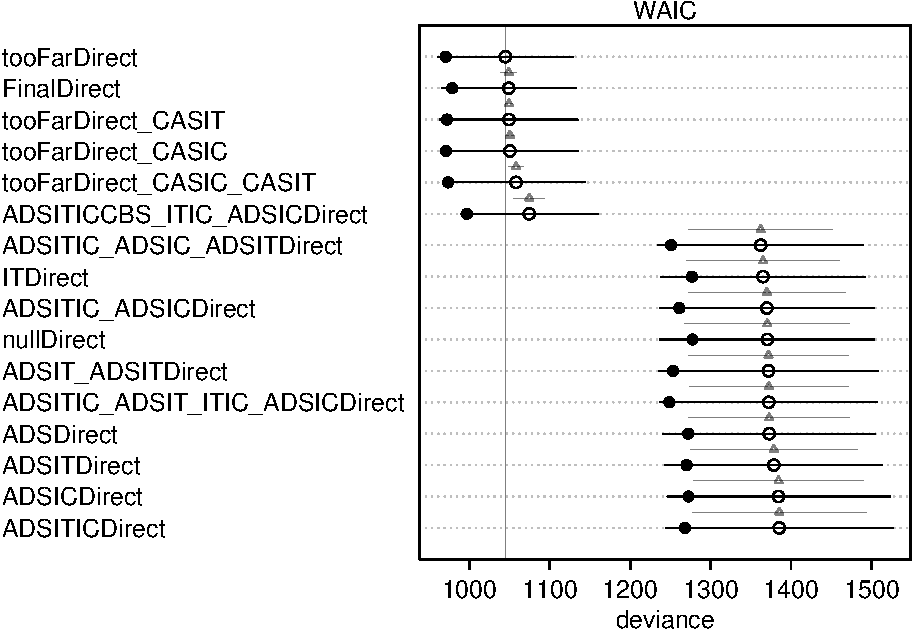
\includegraphics[width=1\linewidth]{bayesianReport3_files/figure-latex/comparisonDirectModels-1} \end{center}

\normalsize

Let's build a Hamiltonian Monte Carlo with the same formula:

\vspace{1mm} \footnotesize

\begin{Shaded}
\begin{Highlighting}[]
\CommentTok{# tooFarDirectHMC <- ulam(}
\CommentTok{#   alist(}
\CommentTok{#     AdiffS ~ dnorm( mu, sigma ),}
\CommentTok{#     mu <- a + bADS[groupID] * ADS +  bIT[groupID] + bIC[groupID] * IC + }
\CommentTok{#       bADSIC * ADS * IC+ bCBS[groupID] *CBS + bCBSIC * CBS * IC + bCAS * CAS, }
\CommentTok{#     a ~ dnorm (0,0.3),}
\CommentTok{#     bADS[groupID] ~ dnorm(0,.3),}
\CommentTok{#     bADSIC ~ dnorm(0,.3),}
\CommentTok{#     bCAS ~ dnorm(0,0.3),}
\CommentTok{#     bCBS[groupID] ~ dnorm(0,.3),}
\CommentTok{#     bIT[groupID] ~ dnorm(0,.3),}
\CommentTok{#     bIC[groupID] ~ dnorm(0,.3),}
\CommentTok{#     bCBSIC ~ dnorm(0, .3),}
\CommentTok{#     sigma  ~ dexp(1)}
\CommentTok{#   ), }
\CommentTok{#   data = summaries}
\CommentTok{# )}


\CommentTok{#saveRDS(tooFarDirectHMC, file = "models/tooFarDirectHMC.rds")}

\NormalTok{tooFarDirectHMC <-}\StringTok{ }\KeywordTok{readRDS}\NormalTok{(}\DataTypeTok{file =} \StringTok{"models/tooFarDirectHMC.rds"}\NormalTok{)}
\end{Highlighting}
\end{Shaded}

\normalsize

For a big picture, let's look at predicted direct effect by group and
user activity profile.

\vspace{1mm} \footnotesize

\begin{Shaded}
\begin{Highlighting}[]
\NormalTok{visGroupDirect <-}\StringTok{ }\ControlFlowTok{function}\NormalTok{ (model, ADS, CBS, CAS, }\DataTypeTok{xmin =}\DecValTok{2}\NormalTok{, }\DataTypeTok{ymax =} \DecValTok{-3}\NormalTok{)}
\NormalTok{\{}
\NormalTok{  groupID <-}\StringTok{ }\DecValTok{1}\OperatorTok{:}\DecValTok{3}
\NormalTok{  IC <-}\StringTok{ }\DecValTok{5} 
\NormalTok{  data <-}\StringTok{ }\KeywordTok{expand.grid}\NormalTok{(}\DataTypeTok{ADS =}\NormalTok{ ADS,}\DataTypeTok{groupID =}\NormalTok{ groupID, }\DataTypeTok{CBS =}\NormalTok{ CBS, }\DataTypeTok{CAS =}\NormalTok{ CAS, }\DataTypeTok{IC =}\NormalTok{  IC)}
\NormalTok{  posterior <-}\StringTok{ }\KeywordTok{extract.samples}\NormalTok{(model, }\DataTypeTok{n =} \FloatTok{1e5}\NormalTok{)}
\NormalTok{  mu <-}\StringTok{ }\KeywordTok{link}\NormalTok{( model, }\DataTypeTok{data=}\NormalTok{data ) }
  \KeywordTok{colnames}\NormalTok{(mu) <-}\StringTok{ }\KeywordTok{levels}\NormalTok{(summaries}\OperatorTok{$}\NormalTok{group)}
\NormalTok{  muLong <-}\StringTok{ }\KeywordTok{melt}\NormalTok{(mu)}
  \KeywordTok{colnames}\NormalTok{(muLong) <-}\StringTok{ }\KeywordTok{c}\NormalTok{(}\StringTok{"id"}\NormalTok{, }\StringTok{"group"}\NormalTok{, }\StringTok{"AdiffS"}\NormalTok{)}
\NormalTok{  means <-}\StringTok{  }\KeywordTok{round}\NormalTok{(}\KeywordTok{apply}\NormalTok{(mu , }\DecValTok{2}\NormalTok{ , mean ), }\DecValTok{2}\NormalTok{)}
\NormalTok{  mu_HPDI <-}\StringTok{ }\KeywordTok{round}\NormalTok{(}\KeywordTok{apply}\NormalTok{( mu , }\DecValTok{2}\NormalTok{ , HPDI ),}\DecValTok{2}\NormalTok{)}
\NormalTok{  means <-}\StringTok{ }\KeywordTok{as.data.frame}\NormalTok{(means)}
\NormalTok{  means}\OperatorTok{$}\NormalTok{group <-}\StringTok{ }\KeywordTok{rownames}\NormalTok{(means)}
  \KeywordTok{rownames}\NormalTok{(means) <-}\StringTok{ }\OtherTok{NULL}
\NormalTok{  meansDisp <-}\StringTok{ }\KeywordTok{cbind}\NormalTok{(means,}\KeywordTok{t}\NormalTok{(}\KeywordTok{as.data.frame}\NormalTok{(mu_HPDI)))}
\NormalTok{  meansDisp <-}\StringTok{ }\NormalTok{meansDisp[,}\KeywordTok{c}\NormalTok{(}\DecValTok{1}\NormalTok{,}\DecValTok{3}\NormalTok{,}\DecValTok{4}\NormalTok{)]}
  
\NormalTok{  plot <-}\StringTok{ }\KeywordTok{ggplot}\NormalTok{(muLong)}\OperatorTok{+}\KeywordTok{geom_violin}\NormalTok{(}\KeywordTok{aes}\NormalTok{(}\DataTypeTok{x =}\NormalTok{ group, }\DataTypeTok{y =}\NormalTok{ AdiffS), }\DataTypeTok{alpha =} \FloatTok{0.2}\NormalTok{)}\OperatorTok{+}
\StringTok{    }\KeywordTok{xlab}\NormalTok{(}\StringTok{""}\NormalTok{)}\OperatorTok{+}
\StringTok{    }\KeywordTok{labs}\NormalTok{(}\DataTypeTok{title =} \KeywordTok{paste}\NormalTok{(}\StringTok{"ADS="}\NormalTok{, ADS, }\StringTok{", CBS="}\NormalTok{,  CBS, }\StringTok{", CAS="}\NormalTok{, CAS,  }\DataTypeTok{sep =} \StringTok{""}\NormalTok{))}\OperatorTok{+}
\StringTok{    }\KeywordTok{theme_tufte}\NormalTok{()}\OperatorTok{+}\KeywordTok{ylim}\NormalTok{(}\KeywordTok{c}\NormalTok{(}\OperatorTok{-}\DecValTok{4}\NormalTok{,}\DecValTok{4}\NormalTok{))}
  \CommentTok{#+   annotation_custom(tableGrob(meansDisp), xmin=xmin,  ymax=ymax)}
  \KeywordTok{return}\NormalTok{(plot)}
\NormalTok{\}}



\NormalTok{visGroupDirect2_}\DecValTok{2}\NormalTok{_}\DecValTok{2}\NormalTok{ <-}\StringTok{  }\KeywordTok{visGroupDirect}\NormalTok{(}\DataTypeTok{model =}\NormalTok{ tooFarDirectHMC, }\DataTypeTok{ADS =} \DecValTok{2}\NormalTok{,}\DataTypeTok{CBS =} \DecValTok{-2}\NormalTok{, }\DataTypeTok{CAS =} \DecValTok{-2}\NormalTok{)}
\NormalTok{visGroupDirect200 <-}\StringTok{  }\KeywordTok{visGroupDirect}\NormalTok{(}\DataTypeTok{model =}\NormalTok{ tooFarDirectHMC, }\DataTypeTok{ADS =} \DecValTok{2}\NormalTok{,}\DataTypeTok{CBS =} \DecValTok{0}\NormalTok{, }\DataTypeTok{CAS =} \DecValTok{0}\NormalTok{)}
\NormalTok{visGroupDirect222 <-}\StringTok{ }\KeywordTok{visGroupDirect}\NormalTok{(}\DataTypeTok{model =}\NormalTok{ tooFarDirectHMC, }\DataTypeTok{ADS =} \DecValTok{2}\NormalTok{,}\DataTypeTok{CBS =} \DecValTok{2}\NormalTok{, }\DataTypeTok{CAS =} \DecValTok{2}\NormalTok{)}

\NormalTok{visGroupDirect0_}\DecValTok{2}\NormalTok{_}\DecValTok{2}\NormalTok{ <-}\StringTok{  }\KeywordTok{visGroupDirect}\NormalTok{(}\DataTypeTok{model =}\NormalTok{ tooFarDirectHMC, }\DataTypeTok{ADS =} \DecValTok{0}\NormalTok{,}\DataTypeTok{CBS =} \DecValTok{-2}\NormalTok{, }\DataTypeTok{CAS =} \DecValTok{-2}\NormalTok{)}
\NormalTok{visGroupDirect000 <-}\StringTok{  }\KeywordTok{visGroupDirect}\NormalTok{(}\DataTypeTok{model =}\NormalTok{ tooFarDirectHMC, }\DataTypeTok{ADS =} \DecValTok{0}\NormalTok{,}\DataTypeTok{CBS =} \DecValTok{0}\NormalTok{, }\DataTypeTok{CAS =} \DecValTok{0}\NormalTok{)}
\NormalTok{visGroupDirect022 <-}\StringTok{ }\KeywordTok{visGroupDirect}\NormalTok{(}\DataTypeTok{model =}\NormalTok{ tooFarDirectHMC, }\DataTypeTok{ADS =} \DecValTok{0}\NormalTok{,}\DataTypeTok{CBS =} \DecValTok{2}\NormalTok{, }\DataTypeTok{CAS =} \DecValTok{2}\NormalTok{)}


\NormalTok{visGroupDirect_}\DecValTok{2}\NormalTok{_}\DecValTok{2}\NormalTok{_}\DecValTok{2}\NormalTok{ <-}\StringTok{  }\KeywordTok{visGroupDirect}\NormalTok{(}\DataTypeTok{model =}\NormalTok{ tooFarDirectHMC, }\DataTypeTok{ADS =} \DecValTok{-2}\NormalTok{,}\DataTypeTok{CBS =} \DecValTok{-2}\NormalTok{, }\DataTypeTok{CAS =} \DecValTok{-2}\NormalTok{)}
\NormalTok{visGroupDirect_}\DecValTok{200}\NormalTok{ <-}\StringTok{  }\KeywordTok{visGroupDirect}\NormalTok{(}\DataTypeTok{model =}\NormalTok{ tooFarDirectHMC, }\DataTypeTok{ADS =} \DecValTok{-2}\NormalTok{,}\DataTypeTok{CBS =} \DecValTok{0}\NormalTok{, }\DataTypeTok{CAS =} \DecValTok{0}\NormalTok{)}
\NormalTok{visGroupDirect_}\DecValTok{222}\NormalTok{ <-}\StringTok{ }\KeywordTok{visGroupDirect}\NormalTok{(}\DataTypeTok{model =}\NormalTok{ tooFarDirectHMC, }\DataTypeTok{ADS =} \DecValTok{-2}\NormalTok{,}\DataTypeTok{CBS =} \DecValTok{2}\NormalTok{, }\DataTypeTok{CAS =} \DecValTok{2}\NormalTok{)}


\NormalTok{visGroupDirectJoint <-}\StringTok{ }\KeywordTok{ggarrange}\NormalTok{(visGroupDirect2_}\DecValTok{2}\NormalTok{_}\DecValTok{2}\OperatorTok{+}\NormalTok{removeX }\OperatorTok{+}\KeywordTok{ylab}\NormalTok{(}\StringTok{"ADS = 2"}\NormalTok{)}\OperatorTok{+}\KeywordTok{ggtitle}\NormalTok{(}\StringTok{"CBS = CAS = -2"}\NormalTok{),}
\NormalTok{                                 visGroupDirect200}\OperatorTok{+}\NormalTok{removeX}\OperatorTok{+}\NormalTok{removeY}\OperatorTok{+}\StringTok{ }\KeywordTok{ggtitle}\NormalTok{(}\StringTok{"CBS = CAS = 0"}\NormalTok{),}
\NormalTok{                                 visGroupDirect222}\OperatorTok{+}\NormalTok{removeX}\OperatorTok{+}\NormalTok{removeY}\OperatorTok{+}\StringTok{ }\KeywordTok{ggtitle}\NormalTok{(}\StringTok{"CBS = CAS = 2"}\NormalTok{) ,}
\NormalTok{                        visGroupDirect0_}\DecValTok{2}\NormalTok{_}\DecValTok{2}\OperatorTok{+}\NormalTok{removeX }\OperatorTok{+}\StringTok{ }\KeywordTok{ggtitle}\NormalTok{(}\StringTok{""}\NormalTok{)}\OperatorTok{+}\KeywordTok{ylab}\NormalTok{(}\StringTok{"ADS = 0"}\NormalTok{),}
\NormalTok{                                visGroupDirect000}\OperatorTok{+}\NormalTok{removeX}\OperatorTok{+}\NormalTok{removeY}\OperatorTok{+}\StringTok{ }\KeywordTok{ggtitle}\NormalTok{(}\StringTok{""}\NormalTok{),}
\NormalTok{                                visGroupDirect022}\OperatorTok{+}\NormalTok{removeX}\OperatorTok{+}\NormalTok{removeY}\OperatorTok{+}\StringTok{ }\KeywordTok{ggtitle}\NormalTok{(}\StringTok{""}\NormalTok{),}
\NormalTok{                        visGroupDirect_}\DecValTok{2}\NormalTok{_}\DecValTok{2}\NormalTok{_}\DecValTok{2}\OperatorTok{+}\NormalTok{removeX}\OperatorTok{+}\KeywordTok{ylab}\NormalTok{(}\StringTok{"ADS = -2"}\NormalTok{)}\OperatorTok{+}\StringTok{ }\KeywordTok{ggtitle}\NormalTok{(}\StringTok{""}\NormalTok{),}
\NormalTok{                                  visGroupDirect_}\DecValTok{200}\OperatorTok{+}\NormalTok{removeX}\OperatorTok{+}\NormalTok{removeY}\OperatorTok{+}\StringTok{ }\KeywordTok{ggtitle}\NormalTok{(}\StringTok{""}\NormalTok{),}
\NormalTok{                        visGroupDirect_}\DecValTok{222}\OperatorTok{+}\NormalTok{removeX}\OperatorTok{+}\NormalTok{removeY}\OperatorTok{+}\StringTok{ }\KeywordTok{ggtitle}\NormalTok{(}\StringTok{""}\NormalTok{)}
\NormalTok{                                 ,}\DataTypeTok{ncol =}\DecValTok{3}\NormalTok{, }\DataTypeTok{nrow =} \DecValTok{3}\NormalTok{)}
                                  
      


\NormalTok{visGroupDirectJoint2 <-}\StringTok{ }\KeywordTok{annotate_figure}\NormalTok{(visGroupDirectJoint, }
                                  \DataTypeTok{top =} \KeywordTok{text_grob}\NormalTok{(}\StringTok{"(range restricted to (-4,4), IC at the rounded mean = 5)"}\NormalTok{,}
                                                  \DataTypeTok{size =} \DecValTok{10}\NormalTok{))}
\NormalTok{visGroupJoint3 <-}\StringTok{ }\KeywordTok{annotate_figure}\NormalTok{(visGroupDirectJoint2, }
                                  \DataTypeTok{top =} \KeywordTok{text_grob}\NormalTok{(}\StringTok{"Predicted direct effect of treatment group by activity profile (standardized)"}\NormalTok{,}
                                                  \DataTypeTok{size =} \DecValTok{12}\NormalTok{))}

\NormalTok{visGroupJoint3}
\end{Highlighting}
\end{Shaded}

\begin{center}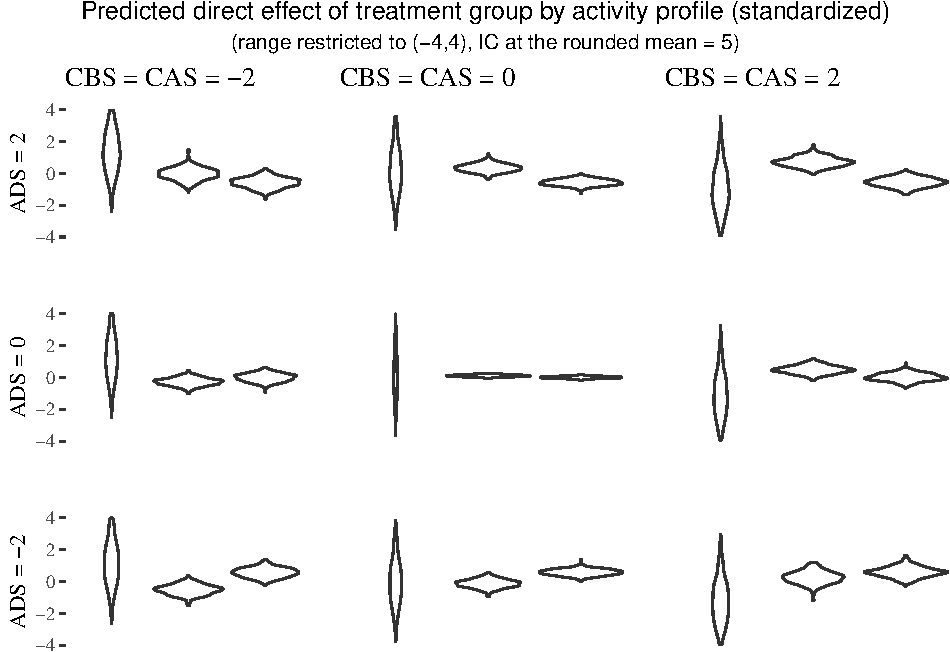
\includegraphics[width=1\linewidth]{bayesianReport3_files/figure-latex/unnamed-chunk-17-1} \end{center}

\normalsize

Now, predicted direct effect of five interventions vs. \textsf{CBS}, for
three user activity profiles.

\vspace{1mm} \footnotesize

\begin{Shaded}
\begin{Highlighting}[]
\NormalTok{visContrastsCBSDirect <-}\StringTok{ }\ControlFlowTok{function}\NormalTok{(}\DataTypeTok{model =}\NormalTok{ FinalHMC, }\DataTypeTok{ADS =}\NormalTok{ ADS , }\DataTypeTok{CAS=}\NormalTok{ CAS, }\DataTypeTok{IC =}  \DecValTok{5}\NormalTok{,}
                            \DataTypeTok{CBS =} \KeywordTok{seq}\NormalTok{(}\OperatorTok{-}\DecValTok{3}\NormalTok{,}\DecValTok{3}\NormalTok{,}\DataTypeTok{by  =} \FloatTok{0.1}\NormalTok{))\{}
\NormalTok{  groupID <-}\StringTok{ }\DecValTok{1}\OperatorTok{:}\DecValTok{3}
\NormalTok{  data <-}\StringTok{ }\KeywordTok{expand.grid}\NormalTok{(ADS, groupID, CAS, IC , CBS)}
  \KeywordTok{colnames}\NormalTok{(data) <-}\StringTok{ }\KeywordTok{c}\NormalTok{(}\StringTok{"ADS"}\NormalTok{, }\StringTok{"groupID"}\NormalTok{, }\StringTok{"CAS"}\NormalTok{, }\StringTok{"IC"}\NormalTok{, }\StringTok{"CBS"}\NormalTok{)}
\NormalTok{  posterior <-}\StringTok{ }\KeywordTok{extract.samples}\NormalTok{(model, }\DataTypeTok{n =} \FloatTok{1e5}\NormalTok{)}
  \KeywordTok{link}\NormalTok{( model, }\DataTypeTok{data=}\NormalTok{data ) }
\NormalTok{  mu <-}\StringTok{ }\KeywordTok{link}\NormalTok{( model, }\DataTypeTok{data=}\NormalTok{data ) }
  
\NormalTok{  means <-}\StringTok{  }\KeywordTok{round}\NormalTok{(}\KeywordTok{apply}\NormalTok{(mu , }\DecValTok{2}\NormalTok{ , mean ), }\DecValTok{4}\NormalTok{)}
  
\NormalTok{  HPDIs <-}\StringTok{ }\KeywordTok{round}\NormalTok{(}\KeywordTok{apply}\NormalTok{( mu , }\DecValTok{2}\NormalTok{ , HPDI ),}\DecValTok{4}\NormalTok{)}
\NormalTok{  visContrast <-}\StringTok{ }\KeywordTok{cbind}\NormalTok{(data,means,}\KeywordTok{t}\NormalTok{(}\KeywordTok{as.data.frame}\NormalTok{(HPDIs)))}
  
\NormalTok{  ones <-}\StringTok{ }\DecValTok{3} \OperatorTok{*}\StringTok{ }\NormalTok{(}\DecValTok{1}\OperatorTok{:}\NormalTok{(}\KeywordTok{nrow}\NormalTok{(visContrast)}\OperatorTok{/}\DecValTok{3}\NormalTok{))}\OperatorTok{-}\DecValTok{2}
\NormalTok{  twos <-}\StringTok{ }\DecValTok{3} \OperatorTok{*}\StringTok{ }\NormalTok{(}\DecValTok{1}\OperatorTok{:}\NormalTok{(}\KeywordTok{nrow}\NormalTok{(visContrast)}\OperatorTok{/}\DecValTok{3}\NormalTok{))}\OperatorTok{-}\DecValTok{1}
\NormalTok{  threes <-}\StringTok{ }\DecValTok{3} \OperatorTok{*}\StringTok{ }\NormalTok{(}\DecValTok{1}\OperatorTok{:}\NormalTok{(}\KeywordTok{nrow}\NormalTok{(visContrast)}\OperatorTok{/}\DecValTok{3}\NormalTok{))}
  
  \KeywordTok{colnames}\NormalTok{(visContrast)[}\KeywordTok{c}\NormalTok{(}\DecValTok{7}\NormalTok{,}\DecValTok{8}\NormalTok{)] <-}\StringTok{ }\KeywordTok{c}\NormalTok{(}\StringTok{"low"}\NormalTok{, }\StringTok{"high"}\NormalTok{)}
  
\NormalTok{  contrast <-}\StringTok{ }\KeywordTok{numeric}\NormalTok{(}\KeywordTok{nrow}\NormalTok{(visContrast))}
\NormalTok{  cLow <-}\StringTok{ }\KeywordTok{numeric}\NormalTok{(}\KeywordTok{nrow}\NormalTok{(visContrast))}
\NormalTok{  cHigh <-}\StringTok{ }\KeywordTok{numeric}\NormalTok{(}\KeywordTok{nrow}\NormalTok{(visContrast))}
  \ControlFlowTok{for}\NormalTok{(i }\ControlFlowTok{in}\NormalTok{ threes)\{}
\NormalTok{    contrast[i] <-}\StringTok{ }\NormalTok{visContrast}\OperatorTok{$}\NormalTok{means[i] }\OperatorTok{-}\StringTok{ }\NormalTok{visContrast}\OperatorTok{$}\NormalTok{means[i}\DecValTok{-2}\NormalTok{]  }
\NormalTok{  \}}
  \ControlFlowTok{for}\NormalTok{(i }\ControlFlowTok{in}\NormalTok{ twos)\{}
\NormalTok{    contrast[i] <-}\StringTok{ }\NormalTok{visContrast}\OperatorTok{$}\NormalTok{means[i] }\OperatorTok{-}\StringTok{ }\NormalTok{visContrast}\OperatorTok{$}\NormalTok{means[i}\DecValTok{-1}\NormalTok{]  }
\NormalTok{  \}}
\NormalTok{  visContrast}\OperatorTok{$}\NormalTok{contrast <-}\StringTok{ }\NormalTok{contrast}
\NormalTok{  visContrast}\OperatorTok{$}\NormalTok{shift <-}\StringTok{  }\NormalTok{visContrast}\OperatorTok{$}\NormalTok{contrast }\OperatorTok{-}\StringTok{ }\NormalTok{visContrast}\OperatorTok{$}\NormalTok{means}
  \ControlFlowTok{for}\NormalTok{(i }\ControlFlowTok{in}\NormalTok{ ones)\{}
\NormalTok{    visContrast}\OperatorTok{$}\NormalTok{shift[i] <-}\StringTok{ }\DecValTok{0}
\NormalTok{  \}}
\NormalTok{  visContrast}\OperatorTok{$}\NormalTok{cLow <-}\StringTok{ }\NormalTok{visContrast}\OperatorTok{$}\NormalTok{low }\OperatorTok{+}\StringTok{ }\NormalTok{visContrast}\OperatorTok{$}\NormalTok{shift}
\NormalTok{  visContrast}\OperatorTok{$}\NormalTok{cHigh <-}\StringTok{ }\NormalTok{visContrast}\OperatorTok{$}\NormalTok{high }\OperatorTok{+}\StringTok{ }\NormalTok{visContrast}\OperatorTok{$}\NormalTok{shift}
  
\NormalTok{  visContrast}\OperatorTok{$}\NormalTok{group =}\StringTok{ }\KeywordTok{rep}\NormalTok{(}\KeywordTok{c}\NormalTok{(}\StringTok{"control"}\NormalTok{, }\StringTok{"empathy"}\NormalTok{, }\StringTok{"normative"}\NormalTok{), }
                          \KeywordTok{nrow}\NormalTok{(visContrast)}\OperatorTok{/}\DecValTok{3}\NormalTok{)}
  
\NormalTok{  visContrastTreatment <-}\StringTok{ }\NormalTok{visContrast[groupID }\OperatorTok{!=}\DecValTok{1}\NormalTok{,]}
  
  \KeywordTok{return}\NormalTok{(}\KeywordTok{ggplot}\NormalTok{(visContrastTreatment, }\KeywordTok{aes}\NormalTok{(}\DataTypeTok{x =}\NormalTok{ CBS, }\DataTypeTok{y =}\NormalTok{ contrast, }\DataTypeTok{fill =}\NormalTok{ group ))}\OperatorTok{+}
\StringTok{           }\KeywordTok{geom_line}\NormalTok{(}\DataTypeTok{se =} \OtherTok{FALSE}\NormalTok{)}\OperatorTok{+}
\StringTok{           }\KeywordTok{geom_ribbon}\NormalTok{(}\DataTypeTok{mapping =} 
                         \KeywordTok{aes}\NormalTok{(}\DataTypeTok{ymin =}\NormalTok{ cLow, }\DataTypeTok{ymax =}\NormalTok{ cHigh),  }
                       \DataTypeTok{alpha =} \FloatTok{.3}\NormalTok{)}\OperatorTok{+}
\StringTok{           }\KeywordTok{theme_tufte}\NormalTok{()}\OperatorTok{+}\KeywordTok{ylim}\NormalTok{(}\KeywordTok{c}\NormalTok{(}\OperatorTok{-}\FloatTok{3.5}\NormalTok{,}\FloatTok{3.5}\NormalTok{)))}
\NormalTok{\}}

\NormalTok{visContrastDirect <-}\StringTok{  }\KeywordTok{ggarrange}\NormalTok{(}\KeywordTok{visContrastsCBSDirect}\NormalTok{(}\DataTypeTok{model =}\NormalTok{ tooFarDirect,}\DataTypeTok{ADS =} \DecValTok{-2}\NormalTok{, }\DataTypeTok{CAS =} \DecValTok{-2}\NormalTok{, }\DataTypeTok{IC =} \DecValTok{5}\NormalTok{)}\OperatorTok{+}\KeywordTok{ggtitle}\NormalTok{(}\StringTok{"ADS = CAS = -2"}\NormalTok{)}\OperatorTok{+}\StringTok{ }\KeywordTok{scale_fill_discrete}\NormalTok{(}\DataTypeTok{guide=}\OtherTok{FALSE}\NormalTok{),}
          \KeywordTok{visContrastsCBSDirect}\NormalTok{(}\DataTypeTok{model =}\NormalTok{ tooFarDirect,}\DataTypeTok{ADS =} \DecValTok{0}\NormalTok{, }\DataTypeTok{CAS =} \DecValTok{0}\NormalTok{, }\DataTypeTok{IC =} \DecValTok{5}\NormalTok{) }\OperatorTok{+}\KeywordTok{ggtitle}\NormalTok{(}\StringTok{"ADS = CAS = 0"}\NormalTok{)}\OperatorTok{+}\StringTok{ }\KeywordTok{scale_fill_discrete}\NormalTok{(}\DataTypeTok{guide=}\OtherTok{FALSE}\NormalTok{)}\OperatorTok{+}\NormalTok{removeY,}
          \KeywordTok{visContrastsCBSDirect}\NormalTok{(}\DataTypeTok{model =}\NormalTok{ tooFarDirect,}\DataTypeTok{ADS =} \DecValTok{2}\NormalTok{, }\DataTypeTok{CAS =} \DecValTok{2}\NormalTok{, }\DataTypeTok{IC =} \DecValTok{5}\NormalTok{) }\OperatorTok{+}\KeywordTok{ggtitle}\NormalTok{(}\StringTok{"ADS = CAS = 2"}\NormalTok{)}\OperatorTok{+}\StringTok{ }\KeywordTok{scale_fill_discrete}\NormalTok{(}\DataTypeTok{guide=}\OtherTok{FALSE}\NormalTok{)}\OperatorTok{+}\NormalTok{removeY}
\NormalTok{          ,}\DataTypeTok{ncol =}\DecValTok{3}\NormalTok{)}
\end{Highlighting}
\end{Shaded}

\begin{verbatim}
## Warning: Ignoring unknown parameters: se

## Warning: Ignoring unknown parameters: se

## Warning: Ignoring unknown parameters: se
\end{verbatim}

\begin{verbatim}
## Warning: It is deprecated to specify `guide = FALSE` to remove a guide. Please
## use `guide = "none"` instead.

## Warning: It is deprecated to specify `guide = FALSE` to remove a guide. Please
## use `guide = "none"` instead.

## Warning: It is deprecated to specify `guide = FALSE` to remove a guide. Please
## use `guide = "none"` instead.
\end{verbatim}

\begin{Shaded}
\begin{Highlighting}[]
\NormalTok{visContrastDirect2 <-}\StringTok{ }\KeywordTok{annotate_figure}\NormalTok{(visContrastDirect, }
                                        \DataTypeTok{top =} \KeywordTok{text_grob}\NormalTok{(}\StringTok{"(range restricted to (-3.5,3.5), IC at the rounded mean = 5)"}\NormalTok{,}
                                                        \DataTypeTok{size =} \DecValTok{10}\NormalTok{))}
\NormalTok{visContrastDirect3 <-}\StringTok{ }\KeywordTok{annotate_figure}\NormalTok{(visContrastDirect2, }
                                        \DataTypeTok{top =} \KeywordTok{text_grob}\NormalTok{(}\StringTok{"Predicted direct effect distance from the control group mean vs. CBS  (standardized)"}\NormalTok{,}
                                                        \DataTypeTok{size =} \DecValTok{12}\NormalTok{))}

\NormalTok{visContrastDirect3}
\end{Highlighting}
\end{Shaded}

\begin{center}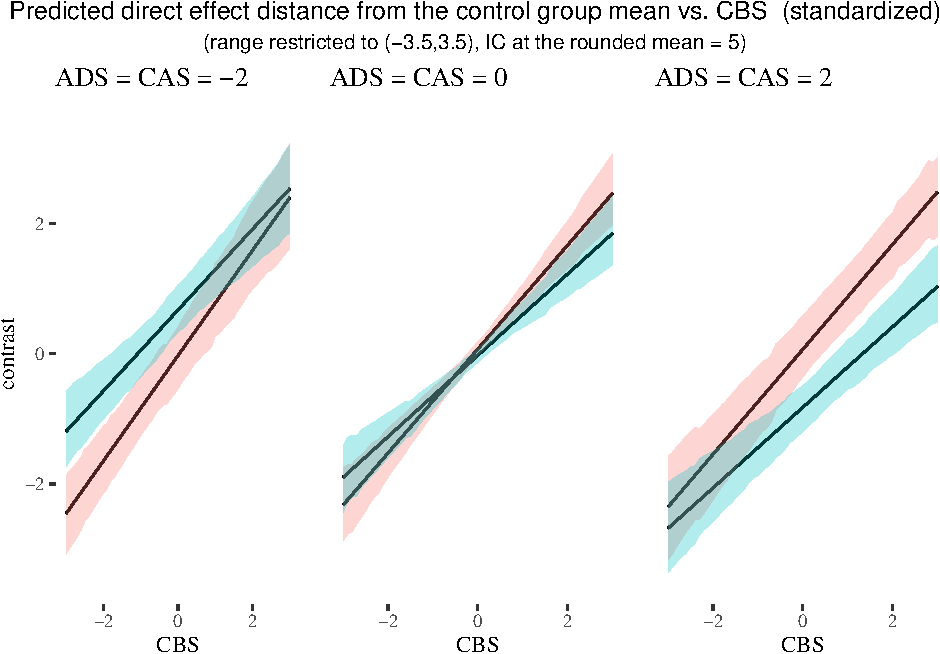
\includegraphics[width=1\linewidth]{bayesianReport3_files/figure-latex/unnamed-chunk-18-1} \end{center}

\normalsize

Now contrasts against \textsf{ADS}, for three user profiles:

\vspace{1mm} \footnotesize

\begin{Shaded}
\begin{Highlighting}[]
\NormalTok{visContrastsADSDirect <-}\StringTok{ }\ControlFlowTok{function}\NormalTok{(}\DataTypeTok{model =}\NormalTok{ FinalHMC, }\DataTypeTok{CBS =}\NormalTok{ CBS , }\DataTypeTok{CAS =}\NormalTok{ CAS, }\DataTypeTok{IC =}  \DecValTok{5}\NormalTok{, }
                            \DataTypeTok{ADS =} \KeywordTok{seq}\NormalTok{(}\OperatorTok{-}\DecValTok{3}\NormalTok{,}\DecValTok{3}\NormalTok{,}\DataTypeTok{by  =} \FloatTok{0.1}\NormalTok{))}
\NormalTok{\{}
\NormalTok{  data <-}\StringTok{ }\KeywordTok{expand.grid}\NormalTok{(CBS, groupID, CAS, IC , ADS)}
  \KeywordTok{colnames}\NormalTok{(data) <-}\StringTok{ }\KeywordTok{c}\NormalTok{(}\StringTok{"CBS"}\NormalTok{, }\StringTok{"groupID"}\NormalTok{, }\StringTok{"CAS"}\NormalTok{, }\StringTok{"IC"}\NormalTok{, }\StringTok{"ADS"}\NormalTok{)}
\NormalTok{  posterior <-}\StringTok{ }\KeywordTok{extract.samples}\NormalTok{(model, }\DataTypeTok{n =} \FloatTok{1e5}\NormalTok{)}
\NormalTok{  mu <-}\StringTok{ }\KeywordTok{link}\NormalTok{( model, }\DataTypeTok{data=}\NormalTok{data ) }
\NormalTok{  means <-}\StringTok{  }\KeywordTok{round}\NormalTok{(}\KeywordTok{apply}\NormalTok{(mu , }\DecValTok{2}\NormalTok{ , mean ), }\DecValTok{4}\NormalTok{)}
\NormalTok{  HPDIs <-}\StringTok{ }\KeywordTok{round}\NormalTok{(}\KeywordTok{apply}\NormalTok{( mu , }\DecValTok{2}\NormalTok{ , HPDI ),}\DecValTok{4}\NormalTok{)}
\NormalTok{  visContrastADS <-}\StringTok{ }\KeywordTok{cbind}\NormalTok{(data,means,}\KeywordTok{t}\NormalTok{(}\KeywordTok{as.data.frame}\NormalTok{(HPDIs)))}
  
  
\NormalTok{  ones <-}\StringTok{ }\DecValTok{3} \OperatorTok{*}\StringTok{ }\NormalTok{(}\DecValTok{1}\OperatorTok{:}\NormalTok{(}\KeywordTok{nrow}\NormalTok{(visContrastADS)}\OperatorTok{/}\DecValTok{3}\NormalTok{))}\OperatorTok{-}\DecValTok{2}
\NormalTok{  twos <-}\StringTok{ }\DecValTok{3} \OperatorTok{*}\StringTok{ }\NormalTok{(}\DecValTok{1}\OperatorTok{:}\NormalTok{(}\KeywordTok{nrow}\NormalTok{(visContrastADS)}\OperatorTok{/}\DecValTok{3}\NormalTok{))}\OperatorTok{-}\DecValTok{1}
\NormalTok{  threes <-}\StringTok{ }\DecValTok{3} \OperatorTok{*}\StringTok{ }\NormalTok{(}\DecValTok{1}\OperatorTok{:}\NormalTok{(}\KeywordTok{nrow}\NormalTok{(visContrastADS)}\OperatorTok{/}\DecValTok{3}\NormalTok{))}
  
  \KeywordTok{colnames}\NormalTok{(visContrastADS)[}\KeywordTok{c}\NormalTok{(}\DecValTok{7}\NormalTok{,}\DecValTok{8}\NormalTok{)] <-}\StringTok{ }\KeywordTok{c}\NormalTok{(}\StringTok{"low"}\NormalTok{, }\StringTok{"high"}\NormalTok{)}
\NormalTok{  contrastADS <-}\StringTok{ }\KeywordTok{numeric}\NormalTok{(}\KeywordTok{nrow}\NormalTok{(visContrastADS))}
  \ControlFlowTok{for}\NormalTok{(i }\ControlFlowTok{in}\NormalTok{ threes)\{}
\NormalTok{    contrastADS[i] <-}\StringTok{ }\NormalTok{visContrastADS}\OperatorTok{$}\NormalTok{means[i] }\OperatorTok{-}\StringTok{ }\NormalTok{visContrastADS}\OperatorTok{$}\NormalTok{means[i}\DecValTok{-2}\NormalTok{]  }
\NormalTok{  \}}
  \ControlFlowTok{for}\NormalTok{(i }\ControlFlowTok{in}\NormalTok{ twos)\{}
\NormalTok{    contrastADS[i] <-}\StringTok{ }\NormalTok{visContrastADS}\OperatorTok{$}\NormalTok{means[i] }\OperatorTok{-}\StringTok{ }\NormalTok{visContrastADS}\OperatorTok{$}\NormalTok{means[i}\DecValTok{-1}\NormalTok{]  }
\NormalTok{  \}}
\NormalTok{  visContrastADS}\OperatorTok{$}\NormalTok{contrast <-}\StringTok{ }\NormalTok{contrastADS}
\NormalTok{  visContrastADS}\OperatorTok{$}\NormalTok{shift <-}\StringTok{  }\NormalTok{visContrastADS}\OperatorTok{$}\NormalTok{contrast }\OperatorTok{-}\StringTok{ }\NormalTok{visContrastADS}\OperatorTok{$}\NormalTok{means}
  \ControlFlowTok{for}\NormalTok{(i }\ControlFlowTok{in}\NormalTok{ ones)\{}
\NormalTok{    visContrastADS}\OperatorTok{$}\NormalTok{shift[i] <-}\StringTok{ }\DecValTok{0}
\NormalTok{  \}}
\NormalTok{  visContrastADS}\OperatorTok{$}\NormalTok{cLow <-}\StringTok{ }\NormalTok{visContrastADS}\OperatorTok{$}\NormalTok{low }\OperatorTok{+}\StringTok{ }\NormalTok{visContrastADS}\OperatorTok{$}\NormalTok{shift}
\NormalTok{  visContrastADS}\OperatorTok{$}\NormalTok{cHigh <-}\StringTok{ }\NormalTok{visContrastADS}\OperatorTok{$}\NormalTok{high }\OperatorTok{+}\StringTok{ }\NormalTok{visContrastADS}\OperatorTok{$}\NormalTok{shift}
  
\NormalTok{  visContrastADS}\OperatorTok{$}\NormalTok{group =}\StringTok{ }\KeywordTok{rep}\NormalTok{(}\KeywordTok{c}\NormalTok{(}\StringTok{"control"}\NormalTok{, }\StringTok{"empathy"}\NormalTok{, }\StringTok{"normative"}\NormalTok{), }
                             \KeywordTok{nrow}\NormalTok{(visContrastADS)}\OperatorTok{/}\DecValTok{3}\NormalTok{)}
\NormalTok{  visContrastTreatmentADS <-}\StringTok{ }\NormalTok{visContrastADS[groupID }\OperatorTok{!=}\DecValTok{1}\NormalTok{,]}
  
  \KeywordTok{return}\NormalTok{(}\KeywordTok{ggplot}\NormalTok{(visContrastTreatmentADS, }\KeywordTok{aes}\NormalTok{(}\DataTypeTok{x =}\NormalTok{ ADS, }\DataTypeTok{y =}\NormalTok{ contrast, }\DataTypeTok{fill =}\NormalTok{ group ))}\OperatorTok{+}
\StringTok{           }\KeywordTok{geom_line}\NormalTok{(}\DataTypeTok{se =} \OtherTok{FALSE}\NormalTok{) }\OperatorTok{+}
\StringTok{           }\KeywordTok{geom_ribbon}\NormalTok{(}\DataTypeTok{mapping =} \KeywordTok{aes}\NormalTok{(}\DataTypeTok{ymin =}\NormalTok{ cLow, }\DataTypeTok{ymax =}\NormalTok{ cHigh), }
                       \DataTypeTok{alpha =} \FloatTok{.3}\NormalTok{) }\OperatorTok{+}\KeywordTok{theme_tufte}\NormalTok{())}
\NormalTok{\}}





\NormalTok{visContrastADSDirectJoint <-}\StringTok{ }\KeywordTok{ggarrange}\NormalTok{(}
  \KeywordTok{visContrastsADSDirect}\NormalTok{(tooFarDirect,}\DataTypeTok{CBS =} \DecValTok{-2}\NormalTok{, }\DataTypeTok{CAS =} \DecValTok{-2}\NormalTok{)}\OperatorTok{+}\KeywordTok{ggtitle}\NormalTok{(}\StringTok{"CBS = CAS = -2"}\NormalTok{)}\OperatorTok{+}\KeywordTok{ylim}\NormalTok{(}\KeywordTok{c}\NormalTok{(}\OperatorTok{-}\DecValTok{3}\NormalTok{,}\DecValTok{3}\NormalTok{))}\OperatorTok{+}\StringTok{ }\KeywordTok{scale_fill_discrete}\NormalTok{(}\DataTypeTok{guide=}\OtherTok{FALSE}\NormalTok{),}
  \KeywordTok{visContrastsADSDirect}\NormalTok{(tooFarDirect, }\DataTypeTok{CBS =} \DecValTok{0}\NormalTok{, }\DataTypeTok{CAS =} \DecValTok{0}\NormalTok{)}\OperatorTok{+}\KeywordTok{ggtitle}\NormalTok{(}\StringTok{"CBS = CAS = 0"}\NormalTok{)}\OperatorTok{+}\KeywordTok{ylim}\NormalTok{(}\KeywordTok{c}\NormalTok{(}\OperatorTok{-}\DecValTok{3}\NormalTok{,}\DecValTok{3}\NormalTok{))}\OperatorTok{+}\StringTok{ }\KeywordTok{scale_fill_discrete}\NormalTok{(}\DataTypeTok{guide=}\OtherTok{FALSE}\NormalTok{),}
  \KeywordTok{visContrastsADSDirect}\NormalTok{(tooFarDirect, }\DataTypeTok{CBS =} \DecValTok{2}\NormalTok{, }\DataTypeTok{CAS =} \DecValTok{2}\NormalTok{)}\OperatorTok{+}\KeywordTok{ggtitle}\NormalTok{(}\StringTok{"CBS = CAS = 2"}\NormalTok{)}\OperatorTok{+}\KeywordTok{ylim}\NormalTok{(}\KeywordTok{c}\NormalTok{(}\OperatorTok{-}\DecValTok{3}\NormalTok{,}\DecValTok{3}\NormalTok{))}\OperatorTok{+}\StringTok{ }\KeywordTok{scale_fill_discrete}\NormalTok{(}\DataTypeTok{guide=}\OtherTok{FALSE}\NormalTok{),}
  \DataTypeTok{ncol =}\DecValTok{3}\NormalTok{)}
\end{Highlighting}
\end{Shaded}

\begin{verbatim}
## Warning: Ignoring unknown parameters: se

## Warning: Ignoring unknown parameters: se

## Warning: Ignoring unknown parameters: se
\end{verbatim}

\begin{verbatim}
## Warning: It is deprecated to specify `guide = FALSE` to remove a guide. Please
## use `guide = "none"` instead.

## Warning: It is deprecated to specify `guide = FALSE` to remove a guide. Please
## use `guide = "none"` instead.

## Warning: It is deprecated to specify `guide = FALSE` to remove a guide. Please
## use `guide = "none"` instead.
\end{verbatim}

\begin{Shaded}
\begin{Highlighting}[]
\NormalTok{visContrastADSDirectJoint2 <-}\StringTok{ }\KeywordTok{annotate_figure}\NormalTok{(visContrastADSDirectJoint, }
                                        \DataTypeTok{top =} \KeywordTok{text_grob}\NormalTok{(}\StringTok{"(range restricted to (-3,3), IC at the rounded mean = 5)"}\NormalTok{,}
                                                        \DataTypeTok{size =} \DecValTok{10}\NormalTok{))}
\NormalTok{visContrastADSDirectJoint3 <-}\StringTok{ }\KeywordTok{annotate_figure}\NormalTok{(visContrastADSDirectJoint2, }
                                        \DataTypeTok{top =} \KeywordTok{text_grob}\NormalTok{(}\StringTok{"Predicted direct effect distance from the control group mean vs. ADS (standardized)"}\NormalTok{,}
                                                        \DataTypeTok{size =} \DecValTok{12}\NormalTok{))}

\NormalTok{visContrastADSDirectJoint3}
\end{Highlighting}
\end{Shaded}

\begin{center}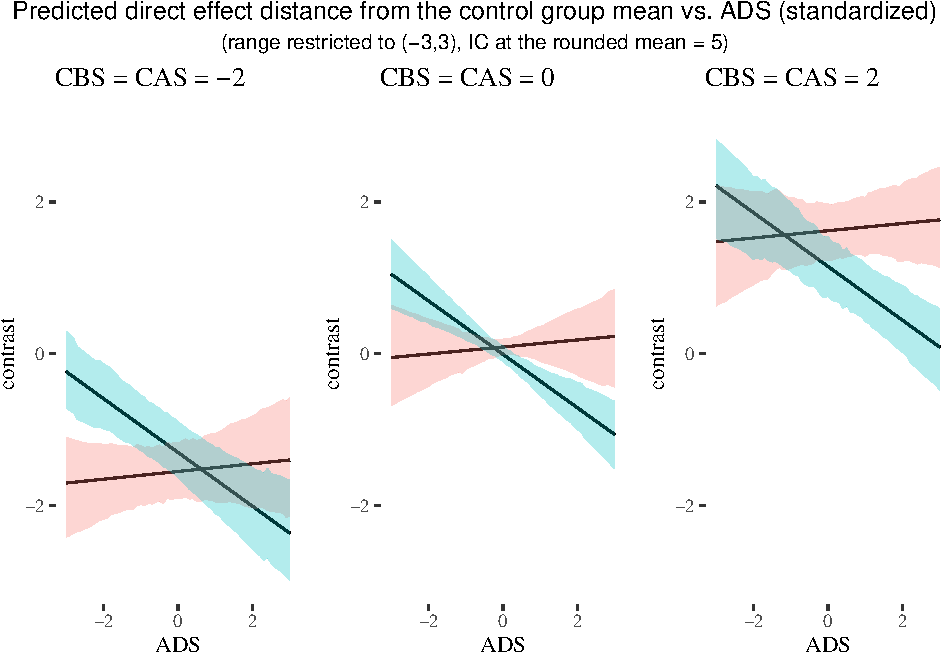
\includegraphics[width=1\linewidth]{bayesianReport3_files/figure-latex/unnamed-chunk-19-1} \end{center}

\normalsize

\section*{References}\label{references}
\addcontentsline{toc}{section}{References}

\vspace{-3mm}

\end{document}
